\def\PageLayout{single-no-print}
\def\DocLanguage{en}
\def\PackagesIncludeTikz{yes}
\def\PackagesIncludeBib{yes}

%%% Please fill in basic information on your thesis, which will be automatically
%%% inserted at the right places. You need to replace ... by real data.

% Type of your thesis:
%	"bc" for Bachelor's
%	"mgr" for Master's
%	"phd" for PhD
%	"rig" for rigorosum
% "sem" for semestral
\def\ThesisType{bc}


\def\ThesisTitle{Surveillance FMCW Radar}

\def\ThesisTitleShort{Surveillance FMCW Radar}

\def\ThesisAuthor{Havránek Kryštof}

\def\MontSubmitted{TODO}

\def\YearSubmitted{2024}

\def\Institution{Czech Technical University in Prague}

\def\Faculty{Faculty of Electrical Engineering}

\def\DepartmentType{Department}

\def\Department{Department of Electromagnetic Field}

\def\Supervisor{Ing. Viktor Adler, Ph.D}

\def\SupervisorsDepartment{Department of Electromagnetic Field}

\def\StudyProgramme{Elektronika a komunikace}

\def\Dedication{%
Dedication.
}

\def\Abstract{%
	TODO
}

% 3 to 5 keywords (recommended) separated by \sep
% Keywords are useful for indexing and searching for the theses by topic.
\def\ThesisKeywords{%
	TODO
}

% If any of your metadata strings contains TeX macros, you need to provide
% a plain-text version for use in XMP metadata embedded in the output PDF file.
% If you are not sure, check the generated thesis.xmpdata file.
\def\AuthorXMP{\ThesisAuthor}
\def\TitleXMP{\ThesisTitle}
\def\KeywordsXMP{\ThesisKeywords}
\def\AbstractXMP{\Abstract}

% If your abstracts are long and do not fit in the infopage, you can make the
% fonts a bit smaller by this setting. (Also, you should try to compress your abstract more.)
\def\InfoPageFont{}
%\def\InfoPageFont{\small}  % uncomment to decrease font size

% If you are studing in a Czech programme, you also need to provide metadata in Czech:
% (in English programmes, this is not used anywhere)

\def\ThesisTitleCS{Přehledový FMCW radar}
\def\DepartmentCS{Katedra elektromagnetického pole}
\def\DepartmentTypeCS{Katedra}
\def\SupervisorsDepartmentCS{Katedra elektromagnetického pole}
\def\StudyProgrammeCS{Elektronika a komunikace}

\def\ThesisKeywordsCS{%
	TODO
}

\def\AbstractCS{%
	TODO
}


%%% Different page dimensions used on thesis
\def\PageLayoutSingle{single}
\def\PageLayoutSingleNoPrint{single-no-print}
\def\PageLayoutDouble{double}
\def\PageLayoutDoubleNoPrint{double-no-print}



%% Single page print
\ifx\PageLayout\PageLayoutSingle
\documentclass[a4paper,oneside,12pt]{report}
\setlength\textwidth{145mm}
\setlength\textheight{251mm}
\setlength\oddsidemargin{15mm}
\setlength\evensidemargin{15mm}
\setlength\topmargin{-0.4in}
\setlength\headsep{10mm}
\setlength\headheight{0mm}
\let\openright=\clearpage
\fi

%% Double page print
\ifx\PageLayout\PageLayoutDouble
% \documentclass[12pt,a4paper,twoside,openright]{report} % chapter will always start on the right side
\documentclass[12pt,a4paper,twoside]{report}
\setlength\textwidth{145mm}
\setlength\textheight{251mm}
\setlength\oddsidemargin{14.2mm}
\setlength\evensidemargin{0mm}
\setlength\topmargin{-0.4in}
\setlength\headsep{10mm}
\setlength\headheight{0mm}
\let\openright=\clearpage
% \let\openright=\cleardoublepage
\fi

%% Double page without space left for binding
\ifx\PageLayout\PageLayoutDoubleNoPrint
% \documentclass[12pt,a4paper,twoside,openright]{report} % chapter will always start on the right side
\documentclass[12pt,a4paper,twoside]{report}
\setlength\textwidth{145mm}
\setlength\textheight{251mm}
\setlength\oddsidemargin{9mm}
\setlength\evensidemargin{9mm}
\setlength\topmargin{-0.4in}
\setlength\headsep{10mm}
\setlength\headheight{0mm}
\let\openright=\clearpage
% \let\openright=\cleardoublepage
\fi

%% Single page without space left for binding
\ifx\PageLayout\PageLayoutSingleNoPrint
\documentclass[12pt,a4paper]{report}
\setlength\textwidth{145mm}
\setlength\textheight{251mm}
\setlength\oddsidemargin{9mm}
\setlength\evensidemargin{9mm}
\setlength\topmargin{-0.4in}
\setlength\headsep{10mm}
\setlength\headheight{0mm}
\let\openright=\clearpage

\fi




\def\LangCS{cs}
\def\LangEN{en}
\def\ConfirmExpr{yes}




%%% TiKz
% Memoize package needs to be loaded as soon as possible, in beamer even before document declaration
\ifx\PackagesIncludeTikz\ConfirmExpr
	\usepackage{memoize}
	\usepackage{collargs}
	\usepackage{tikz}
	\usepackage{tikz-cd}
	\usepackage{circuitikz}
	\mmzset{memo dir=memoize}
	\mmzset{auto={circuitikz}{memoize}}
	\mmzset{auto={tikzcdi}{memoize, verbatim}}
	\mmzset{auto={tikzpicture}{memoize, verbatim}}

	\usetikzlibrary{calc}
	\usetikzlibrary{fadings}
	\usetikzlibrary{shapes.geometric, arrows, positioning}

	\tikzstyle{layerheader} = [rectangle, minimum width=3cm, minimum height=1cm, text centered, draw=black, fill=gray!30]
	\tikzstyle{startstop} = [ellipse, minimum width=3cm, minimum height=1cm, text centered, draw=black, fill=red!30]
	\tikzstyle{process} = [rectangle, minimum width=3cm, minimum height=1cm, text centered, draw=black, fill=blue!20]
	\tikzstyle{decision} = [diamond, minimum width=2.5cm, minimum height=1cm, text centered, draw=black, fill=green!20]
	\tikzstyle{arrow} = [thick,->,>=stealth]
\fi




\ifx\DocLanguage\LangCS
	\usepackage[czech]{babel}
	\babelprovide[transforms = oneletter.nobreak]{czech} % non break on single letter words in czech
\else
	\usepackage[english]{babel}
\fi


\usepackage[T1]{fontenc}
\usepackage[utf8]{inputenc}
\usepackage{lmodern,textcomp}

\usepackage[a-2u]{pdfx}         % adding metadata to pdf with .xmpdata file
\usepackage{graphicx}						% inserting pictures
\usepackage{caption}						%	captions of figures
\usepackage{subcaption} 				% multiple figures in one figure environment
\usepackage{hyperref} 					% handling of hypertext
\usepackage{tabularx}           % table environment
\usepackage{xcolor,colortbl}    % more options for colors
\usepackage{textpos}            % more precise control over positioning of elements
\usepackage{longtable}          % longtable environment to enable multipage tables
\usepackage{fancyhdr}						% custom header and footer
\usepackage{xurl}								% extension to url handeling, allows linebreaks in urls and more special characters
\usepackage{enumitem}           % more options for labeling lists
\usepackage{multicol}           % simplest environment to achieve multiple columns

%%% Math packages
\usepackage{pgfplots}           % graphs
\usepackage{amsmath}						% extension for math
\usepackage{amsthm}							% environment for lemmas, proofs, theorems, etc.
\usepackage{amssymb} 						% math symbols
\usepackage{mathrsfs}  	        % math symbols
\usepackage{mathabx}						% math symbols
\usepackage{mathrsfs} 					% Fancy italic used to denote Hilbert spaces and such
\usepackage{bbm} 							  % blackboard variants of computer Modern fonts useful for number groups, mean value notation
\usepackage{esint} 						  % adds more integrals
\usepackage{accents} 						% multiple mathematical accents
\usepackage{arcs} 							% arcs over and under words
\usepackage{steinmetz} 					% Steinmetz notation for complex numbers
\usepackage{mathtools}


%%% Basic configuration of packages
\def\columnseprulecolor{\color{black}}
\setlength{\columnseprule}{0.3pt}

\hypersetup{pdfborder=0 0 0}
\hypersetup{unicode}
\hypersetup{breaklinks=true}

\pgfplotsset{compat=1.15}

%%% Bibliography
\ifx\PackagesIncludeBib\ConfirmExpr
	\usepackage[backend=biber,style=iso-numeric,sortlocale=cs_CZ, url=true]{biblatex}

	\DeclareFieldFormat{labelnumberwidth}{\mkbibbrackets{#1}} % force biblatex to make brackets around numbers
	\ExecuteBibliographyOptions{maxcitenames=2} % In citation with full bibliography entry cite just two names at max, per ISO 690

	\let\familynameformat=\textsc % Use caps-and-small-caps for family names in ISO 690 style.

	% We want to separate multiple authors in citations by commas
	% (while we use semicolons in the bibliography as per the ISO standard)
	\DeclareDelimFormat[textcite]{multinamedelim}{\addcomma\space}
	\DeclareDelimFormat[textcite]{finalnamedelim}{\space and~}
\fi



%%% Minted
\ifx\PackagesIncludeMinted\ConfirmExpr
	\usepackage{minted}
	\setminted{mathescape,escapeinside=@@,linenos,numbersep=5pt,frame=lines,breaklines,tabsize=2,framesep=2mm}
\fi

%%% This file contains definitions of various useful macros and environments %%%
%%% Please add more macros here instead of cluttering other files with them. %%%

\def\LangCS{cs}
\def\LangEN{en}


%%% Minor tweaks of style

% These macros employ a little dirty trick to convince LaTeX to typeset
% chapter headings sanely, without lots of empty space above them.
% Feel free to ignore.
\makeatletter
\def\@makechapterhead#1{
  {\parindent \z@ \raggedright \normalfont
   \Huge\bfseries \thechapter. #1
   \par\nobreak
   \vskip 20\p@
}}
\def\@makeschapterhead#1{
  {\parindent \z@ \raggedright \normalfont
   \Huge\bfseries #1
   \par\nobreak
   \vskip 20\p@
}}
\makeatother

% make chaptermark non uppercase
\renewcommand{\chaptermark}[1]{%
  \markboth{#1}{}}

% This macro defines a chapter, which is not numbered, but is included in the table of contents.
\def\chapwithtoc#1{
\chapter*{#1}
\addcontentsline{toc}{chapter}{#1}
}

% Slightly less strict rules for placing breaklines inside words
\lefthyphenmin=2
\righthyphenmin=2

% Draw black "slugs" whenever a line overflows, so that we can spot it easily.
% \overfullrule=1mm

% Empty page

\ifx\DocLanguage\LangEN
\newcommand\blankpage{
\newpage
\begin{center}
\vspace*{\fill}
  {Empty page}
\vspace*{\fill}
\end{center}
}

\else
\newcommand\blankpage{
\newpage
\begin{center}
\vspace*{\fill}
  {Prázdná strana}
\vspace*{\fill}
\end{center}
}
\fi


%%% Macros for definitions, theorems, claims, examples, ... (requires amsthm package)
\makeatletter
\def\th@plain{%
  \thm@notefont{}% same as heading font
  \itshape % body font
}
\def\th@definition{%
  \thm@notefont{}% same as heading font
  \normalfont % body font
}
\makeatother

\ifx\DocLanguage\LangEN
\theoremstyle{plain}
\newtheorem{thm}{Theorem}
\newtheorem{lemma}[thm]{Lemma}
\newtheorem{claim}[thm]{Claim}
\newtheorem{defn}{Definition}

\theoremstyle{remark}
\newtheorem*{cor}{Corollary}
\newtheorem*{rem}{Remark}
\newtheorem*{example}{Example}

\else
\theoremstyle{plain}
\newtheorem{thm}{Teorém}
\newtheorem{lemma}[thm]{Lemma}
\newtheorem{claim}[thm]{Tvrzení}
\newtheorem{defn}{Definice}

\theoremstyle{remark}
\newtheorem*{cor}{Důsledek}
\newtheorem*{rem}{Připomínka}
\newtheorem*{example}{Například}

\fi


%%% Tweaks for tables
\newcommand{\pulrad}[1]{\raisebox{1.5ex}[0pt]{#1}}
\newcommand{\mc}[1]{\multicolumn{1}{c}{#1}}
\newcolumntype{C}[1]{>{\centering\arraybackslash}p{#1}}

%%% TODO items
\newcommand{\xxx}[1]{\textcolor{red!}{#1}}


%%% Groups of different numbers, average value
\DeclareMathOperator{\R}{\mathbb{R}}
\DeclareMathOperator{\N}{\mathbb{N}}
\DeclareMathOperator{\Q}{\mathbb{Q}}
\DeclareMathOperator{\C}{\mathbb{C}}
\DeclareMathOperator{\F}{\mathbb{F}}
\DeclareMathOperator{\Z}{\mathbb{Z}}

\DeclareMathOperator{\coord}{\text{coord}}
\DeclareMathOperator{\mgrad}{\text{grad}\,}
\DeclareMathOperator{\mdiv}{\mathrm{div}\,}
\DeclareMathOperator{\mrot}{\mathrm{rot}\,}

%%% Comments inside of mathematical equations, useful for simple substitutions and such
\newcommand{\lcom}{\left\langle\left\langle} %% deprecated
\newcommand{\rcom}{\right\rangle\right\rangle} %% deprecated
\newcommand{\com}[1]{\left\langle\left\langle #1 \right\rangle\right\rangle}

%%% Equals with text over it
\DeclareMathOperator{\eqlh}{\mathrel{\stackrel{\makebox[0pt]{\mbox{\normalfont\tiny L'H}}}{=}}}
\DeclareMathOperator{\eqpp}{\mathrel{\stackrel{\makebox[0pt]{\mbox{\normalfont\tiny PP}}}{=}}}
\newcommand{\eqi}[1]{\mathrel{\stackrel{\makebox[0pt]{\mbox{\normalfont\tiny $#1$}}}{=}}}
\newcommand{\rai}[1]{\mathrel{\stackrel{\makebox[0pt]{\mbox{\normalfont\tiny $#1$}}}{\rightarrow}}}

%% Different lines under text
\newcommand*{\ucheck}[1]{\underaccent{\check}{#1}}
\newcommand*{\uwidecheck}[1]{\underaccent{\widecheck{\hphantom{#1}}}{#1}}
\def\doubleunderline#1{\underline{\underline{#1}}}\makeatletter

%%% Handle " in tikzcd
\newenvironment{tikzcdi}{\shorthandoff{"}\begin{tikzcd}}{\end{tikzcd}\shorthandon{"}}%

%%% Macros for statistics and probability theory
\DeclareMathOperator{\pr}{\textsf{P}}
\DeclareMathOperator{\E}{\textsf{E}\,}
\DeclareMathOperator{\var}{\textrm{var}}
\DeclareMathOperator{\sd}{\textrm{sd}}
\DeclareMathOperator{\ED}{\mathbb{E}}

%%% Other math tweaks
\newcommand{\goto}{\rightarrow}
\newcommand{\gotop}{\stackrel{P}{\longrightarrow}}
\newcommand{\maon}[1]{o(n^{#1})}
\newcommand{\abs}[1]{\left|{#1}\right|}
\ExplSyntaxOn
\NewDocumentCommand{\intd}{m}
{
    \int \clist_map_inline:nn { #1 } { \mathrm{d} ##1 \, }
}
\ExplSyntaxOff % expands \intd{x,y} into \int \mathrm{d}x \mathrm{d}y, used primarily in quantum physics
\newcommand{\isqr}[1]{\frac{1}{\sqrt{#1}}}
\newcommand{\T}[1]{#1^\top}

%% braket notation
\DeclarePairedDelimiter\bra{\langle}{\rvert}
\DeclarePairedDelimiter\ket{\lvert}{\rangle}
\DeclarePairedDelimiterX\braket[2]{\langle}{\rangle}{#1\,\delimsize\vert\,\mathopen{}#2}

%%% Environment with different font size
\newenvironment{localsize}[1]
{%
  \clearpage
  \let\orignewcommand\newcommand
  \let\newcommand\renewcommand
  \makeatletter
  \input{bk#1.clo}%
  \makeatother
  \let\newcommand\orignewcommand
}
{%
  \clearpage
}

%%% Prostředí pro tabulky s centrováním textu v buňce
\newcolumntype{C}[1]{>{\centering\arraybackslash}p{#1}}


% Generate XMP metadata file (*.xmpdata)
% one needs to set AuthorXMP, TitleXMP, KeywordsXMP, AbstractXMP

{
\catcode`\%=12
\global\edef\percenthack{%}
}

{
\def\xxx#1{#1}
\def\sep{\string\sep\space}
\let~=\space

\newwrite\xmp
\immediate\openout\xmp=\jobname.xmpdata
\immediate\write\xmp{\percenthack\space Generated automatically from metadata.tex}
\def\xmpitem#1#2{\immediate\write\xmp{\string#1{#2}}}
\xmpitem\Author\AuthorXMP
\xmpitem\Title\TitleXMP
\xmpitem\Keywords\KeywordsXMP
\xmpitem\Subject\AbstractXMP
\xmpitem\Publisher{Czech Technical University in Prague}
\immediate\closeout\xmp
}


\def\PageLayoutSingle{single}
\def\PageLayoutSingleNoPrint{single-no-print}
\def\PageLayoutDouble{double}
\def\PageLayoutDoubleNoPrint{double-no-print}

% Overwrite default chapter behaviour to control what style is used
\makeatletter
    \let\stdchapter\chapter
    \renewcommand*\chapter{%
    \@ifstar{\starchapter}{\@dblarg\nostarchapter}}
    \newcommand*\starchapter[1]{%
        \stdchapter*{#1}
        \thispagestyle{plain}
        \markboth{\MakeUppercase{#1}}{}
    }
    \def\nostarchapter[#1]#2{%
        \stdchapter[{#1}]{#2}
        \thispagestyle{fancy}
    }
\makeatother




%%% Style for TOC, introduction, conclusion, bibliography and such
\fancypagestyle{plain}{
  \fancyhf{}
  \renewcommand{\headrulewidth}{0.4pt}
  \renewcommand{\footrulewidth}{0.4pt}
  \fancyhead[C]{}
  \fancyhead[L]{}
  \fancyfoot[L]{\Institution}
  \fancyfoot[C]{}
  \fancyfoot[R]{\thepage}
}

\ifx\PageLayout\PageLayoutDouble
\fancypagestyle{fancy}{%
  \fancyhf{}%
  \renewcommand{\headrulewidth}{0.4pt}%
  \renewcommand{\footrulewidth}{0.4pt}%
  \fancyhead[C]{}
	\fancyhead[LE]{\textbf{\thechapter. \leftmark}}
	\fancyhead[RO]{\textbf{\rightmark}}
  \fancyfoot[L]{\Institution}
  \fancyfoot[C]{}
  \fancyfoot[R]{\thepage}
}
\fi

\ifx\PageLayout\PageLayoutDoubleNoPrint
\fancypagestyle{fancy}{%
  \fancyhf{}%
  \renewcommand{\headrulewidth}{0.4pt}%
  \renewcommand{\footrulewidth}{0.4pt}%
  \fancyhead[C]{}
	\fancyhead[LE]{\textbf{\thechapter. \leftmark}}
	\fancyhead[RO]{\textbf{\rightmark}}
  \fancyfoot[L]{\Institution}
  \fancyfoot[C]{}
  \fancyfoot[R]{\thepage}
}
\fi


\ifx\PageLayout\PageLayoutSingle
\fancypagestyle{fancy}{%
  \fancyhf{}%
  \renewcommand{\headrulewidth}{0.4pt}%
  \renewcommand{\footrulewidth}{0.4pt}%
  \fancyhead[C]{}
	\fancyhead[L]{\textbf{\thechapter. \leftmark}}
  \fancyfoot[L]{\Institution}
  \fancyfoot[C]{}
  \fancyfoot[R]{\thepage}
}

\fi

\ifx\PageLayout\PageLayoutSingleNoPrint
\fancypagestyle{fancy}{%
  \fancyhf{}%
  \renewcommand{\headrulewidth}{0.4pt}%
  \renewcommand{\footrulewidth}{0.4pt}%
  \fancyhead[C]{}
	\fancyhead[L]{\textbf{\thechapter. \leftmark}}
  \fancyfoot[L]{\Institution}
  \fancyfoot[C]{}
  \fancyfoot[R]{\thepage}
	}

\fi


\addbibresource{bibliography.bib}
\usepackage{pdfpages}

\newcommand{\sirad}{SiRad Easy\textsuperscript{\copyright} }
\newcommand{\boldred}[1]{\textbf{\textcolor{red}{#1}}}
\newcommand{\boldblue}[1]{\textbf{\textcolor{blue}{#1}}}
% \newcommand{\red}[1]{\textcolor{red}{#1}}


\begin{document}

%%% TitlePage

\def\TypeBc{bc}
\def\TypeMgr{mgr}
\def\TypePhD{phd}
\def\TypeRig{rig}
\def\TypeSem{sem}

\ifx\ThesisType\TypeBc
\def\ThesisTypeName{bachelor}
\def\ThesisTypeTitle{BACHELOR THESIS}
\fi

\ifx\ThesisType\TypeMgr
\def\ThesisTypeName{master}
\def\ThesisTypeTitle{MASTER THESIS}
\fi

\ifx\ThesisType\TypePhD
\def\ThesisTypeName{doctoral}
\def\ThesisTypeTitle{DOCTORAL THESIS}
\fi

\ifx\ThesisType\TypeRig
\def\ThesisTypeName{rigorosum}
\def\ThesisTypeTitle{RIGOROSUM THESIS}
\fi

\ifx\ThesisType\TypeSem
\def\ThesisTypeName{semestral}
\def\ThesisTypeTitle{SEMESTRAL PROJECT}
\fi

\pagestyle{empty}
\hypersetup{pageanchor=false}

\begin{center}

{\LARGE\bfseries\Institution}

\vspace{-18mm}
\vfill

{\LARGE\Department}

\vfill

\centerline{\mbox{\def\svgwidth{\columnwidth}\scalebox{0.28}{%% Creator: Inkscape 1.1.2 (0a00cf5339, 2022-02-04), www.inkscape.org
%% PDF/EPS/PS + LaTeX output extension by Johan Engelen, 2010
%% Accompanies image file 'logo.pdf' (pdf, eps, ps)
%%
%% To include the image in your LaTeX document, write
%%   \input{<filename>.pdf_tex}
%%  instead of
%%   \includegraphics{<filename>.pdf}
%% To scale the image, write
%%   \def\svgwidth{<desired width>}
%%   \input{<filename>.pdf_tex}
%%  instead of
%%   \includegraphics[width=<desired width>]{<filename>.pdf}
%%
%% Images with a different path to the parent latex file can
%% be accessed with the `import' package (which may need to be
%% installed) using
%%   \usepackage{import}
%% in the preamble, and then including the image with
%%   \import{<path to file>}{<filename>.pdf_tex}
%% Alternatively, one can specify
%%   \graphicspath{{<path to file>/}}
%%
%% For more information, please see info/svg-inkscape on CTAN:
%%   http://tug.ctan.org/tex-archive/info/svg-inkscape
%%
\begingroup%
  \makeatletter%
  \providecommand\color[2][]{%
    \errmessage{(Inkscape) Color is used for the text in Inkscape, but the package 'color.sty' is not loaded}%
    \renewcommand\color[2][]{}%
  }%
  \providecommand\transparent[1]{%
    \errmessage{(Inkscape) Transparency is used (non-zero) for the text in Inkscape, but the package 'transparent.sty' is not loaded}%
    \renewcommand\transparent[1]{}%
  }%
  \providecommand\rotatebox[2]{#2}%
  \newcommand*\fsize{\dimexpr\f@size pt\relax}%
  \newcommand*\lineheight[1]{\fontsize{\fsize}{#1\fsize}\selectfont}%
  \ifx\svgwidth\undefined%
    \setlength{\unitlength}{76.00125bp}%
    \ifx\svgscale\undefined%
      \relax%
    \else%
      \setlength{\unitlength}{\unitlength * \real{\svgscale}}%
    \fi%
  \else%
    \setlength{\unitlength}{\svgwidth}%
  \fi%
  \global\let\svgwidth\undefined%
  \global\let\svgscale\undefined%
  \makeatother%
  \begin{picture}(1,1.0179701)%
    \lineheight{1}%
    \setlength\tabcolsep{0pt}%
    \put(0,0){
\includegraphics[width=\unitlength,page=1]{img/logo.pdf}}%
  \end{picture}%
\endgroup%
}}}

\vspace{-8mm}
\vfill

{\bf\Large \ThesisTypeTitle}

\vfill


\vspace{15mm}

{\LARGE\bfseries\ThesisTitle}


\vfill


{
\centerline{\vbox{\halign{\hbox to 0.45\hsize{\hfil #}&\hskip 0.5em\parbox[t]{0.45\hsize}{\raggedright #}\cr
Supervisor of the \ThesisTypeName{} thesis:&\Supervisor \cr
\ifx\ThesisType\TypeRig\else
\noalign{\vspace{2mm}}
Study programme:&\StudyProgramme \cr
\fi
}}}}

\vspace{15mm}
Prague \MontSubmitted \ \YearSubmitted

\end{center}



\includepdf{../img/Declaration.pdf}
\newpage
\hypersetup{pageanchor=true}
\protect\pagestyle{plain}
\pagenumbering{roman}


\openright

{\InfoPageFont

\vtop to 0.46\vsize{
\setlength\parindent{0mm}
\setlength\parskip{5mm}

\textbf{Title:} \ThesisTitle \\
\textbf{Author:} \ThesisAuthor \\
\textbf{\DepartmentType:} \Department \\
\textbf{Supervisor:} \Supervisor, \SupervisorsDepartment \\

\textbf{Abstract:}  \Abstract \\

\textbf{Keywords:}
{\def\sep{\unskip, }\ThesisKeywords}

\vfil
}


\vtop to 0.46\vsize{
\setlength\parindent{0mm}
\setlength\parskip{5mm}

\textbf{Název práce:} \ThesisTitleCS \\
\textbf{Autor:} \ThesisAuthor \\
\textbf{\DepartmentTypeCS:} \DepartmentCS \\
\textbf{Vedoucí práce:} \Supervisor, \SupervisorsDepartmentCS \\

\textbf{Abstrakt:} \AbstractCS \\

\textbf{Klíčová slova:}
{\def\sep{\unskip, }\ThesisKeywordsCS}

\vfil
}
}


\newpage

\openright



\tableofcontents

\newpage
\pagenumbering{arabic}
\setcounter{page}{1}


\chapter*{Abbreviations}
\addcontentsline{toc}{chapter}{Abbreviations}


\begin{center}
  \begin{tabular}{| m{4cm}| m{9cm} | }
    \hline
    \textbf{Abbreviation} & \textbf{Meaning}                                            \\
    \hline
    \hline
    AGC                   & Automatic Gain Control                                      \\
    CFAR                  & Constant False Alarm Rate                                   \\
    CW                    & Continuous Wave                                             \\
    DBSCAN                & Density-Based Spatial Clustering of Applications with Noise \\
    DFT                   & Discrete Fourier Transform                                  \\
    devkit                & Development Kit                                             \\
    FFT                   & Fast Fourier Transform                                      \\
    FMCW                  & Frequency Modulated Continuous Wave                         \\
    MCPWM                 & Motor Control Pulse Width Modulation                        \\
    MIMO                  & Multiple Input Multiple Output                              \\
    PCNT                  & Pulse Counter                                               \\
    RCS                   & Radar Cross Section                                         \\
    RMT                   & Remote Control Transceiver                                  \\
    SIMD                  & Single Instruction, Multiple Data                           \\
    SISO                  & Single Input Single Output                                  \\
    SNR                   & Signal to Noise Ratio                                       \\
    TSV                   & Tab Separated Values                                        \\
    \hline
  \end{tabular}

\end{center}



\chapter*{Introduction}
\addcontentsline{toc}{chapter}{Introduction}

The following thesis concerns the realization of a generic surveillance radar system based on FMCW (Frequency-Modulated Continuous Wave) technology.
Conventional FMCW-based surveillance radars often employ multiple receiving antennas or are implemented as MIMO (Multiple-Input Multiple-Output) systems.
In MIMO configurations, electronic beam steering is possible, enabling a larger field of view and the detection of targets in both elevation and azimuth.
Simpler systems, which use only multiple receiving antennas, typically allow for azimuth estimation through phase difference analysis \cite{sandeep2018}.
However, such systems generally require significant processing power and are not capable of providing comprehensive 3D spatial information due to their limited field of view.

To address these limitations, this work proposes a simpler approach: a radar system with just a single RX and TX antenna, where the beam is steered mechanically using a rotary platform.
Initially, the capabilities of the \sirad evaluation board are assessed, followed by the development of a custom two-axis rotary platform.
Both components are then integrated into a unified system, controlled and managed via a MATLAB desktop application.
This integration involves both hardware—namely the rotary platform—and software, including control of the platform and processing of radar data.
Similar systems have been previously developed -- both those relying on a single axis of rotation~\cite{nowok2017, vivet2013} or complex commercial solutions enabling surveillance of the whole 3D space~\cite{blighter}.

FMCW radar operates by transmitting a continuous wave signal whose frequency is modulated over time.
By mixing the transmitted and received signals, harmonic components are produced, with frequencies proportional to the distance of a target \cite{graham2005}.
Applying a Fourier transform to the mixed signal enables the determination of object distances within the scene.
Compared to pulsed radar, FMCW can provide accurate distance measurements with relatively low power consumption \cite{jankiraman2018}.
Velocity estimation is also possible by exploiting the Doppler effect.
However it's nature is more complex than in pulsed systems.


This thesis focuses on the \sirad radar system—a low-cost evaluation board designed to familiarize users with FMCW technology, offering both 24~GHz and 122~GHz headers \cite{siradMAN}.
This versatility allows for a wide range of applications, with detection ranges from a few meters up to 400~meters under ideal conditions \cite{siradMANOld}.
However, due to its relatively low sampling rate and the use of a modest microcontroller, the \sirad is not particularly well-suited for speed measurement: the maximum measurable velocities are well below one meter per second, and even then, measurement accuracy is limited.

To complement the radar, a custom rotary platform was designed and constructed for this thesis.
While commercial solutions exist \cite{standa, carl}, they are often prohibitively expensive and include unnecessary features.
Therefore, a more affordable platform was built from off-the-shelf and 3D-printed components, controlled by an ESP32C6 microcontroller.
This controller interprets G-code-like commands and drives the stepper motors.

Data from both the radar and the platform are processed and visualized within MATLAB.
The processing pipeline follows standard approaches, utilizing techniques such as FFT (Fast Fourier Transform) and CFAR (Constant False Alarm Rate) \cite{richards2022}.
Still, a number of processing steps can be toggled or adjusted by the user, providing considerable flexibility.
Processed data are stored in radar cubes -- a common structure in radar applications \cite{richards2022}; which facilitates the implementation of more advanced post-processing algorithms.
For visualization, the system supports both 2D and 3D representations.

The thesis is organized into five main chapters.
The first provides the theoretical background of FMCW radar technology and its advantages over alternative radar methods.
The second chapter focuses on the \sirad evaluation board, particularly its suitability for surveillance radar applications.
The third chapter describes the design requirements and development process of the custom rotary platform, including its control software.
The fourth chapter gives an overview of the MATLAB desktop application used to control the system and process radar data.
Finally, the fifth chapter delves deeper into the data processing pipeline and available visualization methods.


\pagestyle{fancy}

\chapter{FMCW Radar Fundamentals}

Classical CW (Continuous Wave) radars broadcast a signal only on a single frequency, while FMCW (Frequency-Modulated Continuous Wave) radars make a linear sweep across a given bandwidth.
This approach enables accurate range estimation at low power consumption and still allows speed measurements using the Doppler shift.
However, velocity calculations in FMCW radars are more complex compared to those in single-frequency CW radars.

The "MW" suffix in FMCW radar denotes that the system operates in the microwave frequency range.
These high frequencies enable the use of compact antenna arrays, which can sometimes even be integrated directly on-chip.
Additionally, the millimeter-wave portion of the spectrum is typically license-free \cite{spektrumCTU} and offers large bandwidths, reducing a risk of interference.

\section{Comparison FMCW Radar to Pulse Radar}

Distance measurement using radar predates FMCW technology by several decades.
Early radar systems primarily relied on pulsed signals, where distance can be calculated from the time of flight, $t$, of the signal as
\begin{equation}
  d = \frac{c_o \cdot t}{2}.
  \label{eq:distance}
\end{equation}
Speed calculation is also relatively straightforward, as the Doppler effect is quite clear
\begin{equation}
  v = \frac{f_\mathrm{dop} c_o}{2f_\mathrm{rad}},
  \label{eq:dopler}
\end{equation}
where $f_\mathrm{dop}$ is the Doppler frequency, $c_o$ is the speed of light and $f_\mathrm{rad}$ is the frequency of the radar signal \cite{jankiraman2018}.

While this approach is conceptually straightforward, it has several limitations, particularly in applications requiring high precision at close range.
Achieving fine resolution in distance measurement necessitates very short pulses.
However, to maintain sufficient signal-to-noise ratio (SNR), the transmitted pulse power per pulse must remain high, regardless of its width \cite{jankiraman2018}.

Maintaining high average transmission power poses legal and technical challenges.
Risk of interference with other devices is increased and such system demand bulky, high-power circuitry -- often with high voltages and even vacuum tubes.
Consequently, pulsed radar is predominantly used in applications where fine range resolution is not essential, such as long-range target detection.

One key advantage of pulsed radar is its relatively simple data processing.
In contrast, FMCW radar data processing is more complex due to the interdependence of distance and velocity measurements.
Both distance and velocity of a target cause frequency changes in the received signal.

\section{Basic principles of ideal FMCW radar}

Let us picture an ideal FMCW radar system placed in a scene with a single large target that reflects all incoming signals.
The radar is broadcasting with a periodically repeated frequency sweep from $f_\mathrm{c}$ to $f_\mathrm{c}+BW$ creating a sawtooth waveform.
Aside from a sawtooth, other modulations are also frequently used, such as linear triangular modulation or segmented linear frequency modulation.
These offer some advantages, but the nature of the beat signal, which forms a sine wave with sawtooth modulation, is more complex.
This is especially true in the case of triangle modulations when multiple targets are present \cite{jankiraman2018}.
\sirad kit, used in this thesis, technically uses a segmented linear frequency modulation due to its limited computational power \cite{siradPRO}, but the mathematical principles are similar to those for sawtooth.

\begin{figure}[h!]
  \centering
  \begin{tikzpicture}[>=latex, scale=1]

    % Axes
    \draw[->] (0, 0) -- (8, 0) node[below] {$t$};
    \draw[->] (0, 0) -- (0, 5) node[left] {$f$};

    % Horizontal lines for BW
    \draw[dashed] (0, 4.5) -- (7.5, 4.5);
    \draw[dashed] (0, 1) -- (7.5, 1);
    \draw[dashed] (2.5, -0.05) -- (2.5, 4.7);

    % Labels for fc and BW
    \node[left] at (0, 1) {$f_c$};
    \draw[<->] (-0.5, 1) -- (-0.5, 4.5) node[midway,left] {$BW$};

    % Triangular wave for Tx
    \draw[thick,blue] (0, 1) -- (2.5, 4.5);
    \draw[thick,blue]	(2.5, 1) -- (5, 4.5);
    \draw[thick, dashed, blue] (5, 1) -- (6, 2.4);

    % Triangular wave for Rx (offset version)
    \draw[thick,red] (0.5, 1) -- (3, 4.5);
    \draw[thick,red] (3, 1) -- (5.5, 4.5);
    \draw[thick, dashed, red] (5.4, 1) -- (6.4, 2.4);

    % Label for Tch
    \draw[-] (2.5, -0.05) -- (2.5, 0.05) node[below] {$T_{\text{ch}}$};

    % Labels for Tx and Rx
    \node[blue] at (4.2, 4.1) {\small Tx};
    \node[red] at (5.3, 3.7) {\small Rx};

    % Sweep slope and fb
    \draw[<->] (1, 1) arc[start angle=0, end angle=55, radius=1];
    \node at (1.5, 1.3) {\small $k_{\text{sw}}$};
    \draw[<->] (1.5, 2.37) -- (1.5, 3.12) node[above, left] {$f_b$};

    % Small time delay (tau)
    \draw[<->] (2.5, 0.7) -- (3, 0.7) node[midway,below] {$\tau$};

  \end{tikzpicture}

	\caption[Ideal relation of frequency on time for received and sent signal \cite{adler2023}]{Ideal relation of frequency on time for received and sent signal \cite{adler2023}}
  \label{fig:fmcw_ideal}
\end{figure}

We can clearly see that, in a given time $t$, the frequency spread from the sent signal to the received signal is proportional to the time delay $\tau$.
However, performing a simple subtraction in the spectrogram of both signals isn't really feasible; the calculation needs to take a smarter approach.


Let us define the chirp slope $k_\mathrm{sw}$ with which we can describe the change in frequency of the broadcasted signal as
\begin{equation}
  \Delta f_\mathrm{s}(t) = k_\mathrm{sw}t = \frac{BW}{T_\mathrm{ch}} t,
  \label{eq:deltaf}
\end{equation}
where $t$ is the time, ranging 0 to chirp length $T_\mathrm{ch}$.
The standard equation of an frequency modulated signal can be written as
\begin{equation}
  s_\mathrm{t}(t) = A \cos\left(\omega_c t + 2\pi \int_{0}^{t} f_\mathrm{s}(t) \mathrm{d}t\right),
  \label{eq:fm}
\end{equation}
where $A$ is the amplitude of the signal, $\omega_c$ is the carrier frequency and $f(s)$ is the frequency of the signal.
Substituting (\ref{eq:deltaf}) into (\ref{eq:fm}) we get the signal broadcasted by the radar \cite{suleymanov2016}
\begin{equation}
  s_\mathrm{t}(t) = A \cos(\omega_c t + \pi k_\mathrm{sw}t^2).
  \label{eq:fm2}
\end{equation}

The signal bounced back from a target will have the same equation, only shifted by the time delay $\tau$,
\begin{equation}
  s_\mathrm{r}(t) = A \cos(\omega_c (t - \tau) + \pi k_\mathrm{sw}(t - \tau)^2).
  \label{eq:fm3}
\end{equation}
Now we can calculate the product of the two signals; this can be done easily in the real world using a frequency mixer.
The result of the multiplication is  \cite{suleymanov2016}
\begin{align}
  s(t) = s_\mathrm{r}(t) \cdot  s_\mathrm{t}(t) & = \frac{A^2}{2}\cos\left(2(\omega_c - 2\pi k_\mathrm{sw}T_\tau)t + 2\pi k_{sw}t^2 + (\pi k_\mathrm{sw} \tau^2 - \omega_c \tau) \right)+ \nonumber \\
                                                & +\frac{A^2}{2} \cos\left(2\pi k_\mathrm{sw} \tau t + (\omega_c \tau - \pi k_\mathrm{sw} \tau^2)\right).
  \label{eq:fm4}
\end{align}
The first additive term will lead to a signal with a very high frequency, well above $2\omega_c$.
This term doesn't carry any useful information and is usually filtered out -- either by a low-pass filter or the frequency mixer itself.
The second term is the so-called beat signal, whose frequency is directly proportional to the time delay $\tau$.
Deriving the second argument by time, we get the frequency of the beat signal \cite{graham2005}
\begin{equation}
  f_\mathrm{b} = \frac{1}{2\pi}\frac{\partial}{\partial t} \left(2\pi k_\mathrm{sw} \tau t + (\omega_c \tau - \pi k_\mathrm{sw} \tau^2)\right) = k_\mathrm{sw} \tau.
  \label{eq:fb}
\end{equation}

Calculating the distance to a target is now trivial as the delay $\tau$ is equal to the time it takes for the signal to travel to a target and back \cite{graham2005}
\begin{equation}
  R = \frac{c_0 \tau}{2},
  \label{eq:distance2}
\end{equation}
By substituting (\ref{eq:fb}) into (\ref{eq:distance2}), we get the equation for a distance \cite{graham2005}
\begin{equation}
  R = \frac{c_0 f_\mathrm{b}}{2k_\mathrm{sw}}= \frac{c_o f_\mathrm{b} T_{\mathrm{ch}}}{2 BW}.
  \label{eq:distance3}
\end{equation}


\subsection{Limits of Range Measurement}

The maximal distance is given by the time it takes for the signal to travel from the radar to a target and back.
If the distance were greater than the time of a single chirp, the signal would be interpreted as coming from a closer target.
This gives us a maximal limit on the beat frequency, $f_\mathrm{b} = BW$.

However, in most cases, the limit will be imposed not by $T_\mathrm{ch}$ respectively $BW$ but by the sampling frequency $f_\mathrm{s}$.
In order to avoid aliasing, the Nyquist-Shannon theorem must be satisfied, thus limiting the maximal beat frequency to $f_\mathrm{s}/2$ and resulting in a maximal distance of \cite{jankiraman2018}
\begin{equation}
  R = \frac{c_o f_\mathrm{s}}{4k_\mathrm{sw}}.
  \label{eq:distance4max}
\end{equation}

While sampling with frequency $f_\mathrm{s}$ we get $N =\mathrm{f}_\mathrm{s} T_\mathrm{ch}$ samples.
Applying a DFT to the signal we get $N$ samples in spectrum with frequency resolution of
\begin{equation}
  \Delta f_\mathrm{b} = \frac{f_\mathrm{s}}{N} = \frac{1}{T_{ch}}.
  \label{eq:resolution}
\end{equation}
We can see that the resolution of the spectrum is only inversely proportional to the chirp length and doesn't have any relation to the sampling frequency  \cite{jankiraman2018}.
Now we can substitute $\Delta f_\mathrm{b}$ into (\ref{eq:distance3}) to get the minimal distance that can be measured as
\begin{equation}
  \Delta R = \frac{c_o}{2BW}
  \label{eq:distance5min}
\end{equation}
Thus, in order to increase resolution in range, a wider bandwidth is needed \cite{graham2005}.

There are, of course, other effects impeding the resolution of the radar system, such as phase noise around targets or sweep nonlinearity.
Sweep nonlinearity can be either in the ramp itself, leading to decreasing resolution with range (with both linear and quadratic errors present)  \cite{graham2005}, or in sweep recovery (time to return to the start of the sweep), which leads to a constant decrease in resolution \cite{piper1995}.
Both are, however, largely compensated in modern radar systems by using a closed feedback loop  \cite{graham2005}.


\subsection{Speed Measurement}

In order to demonstrate the effect of moving target on the beat frequency, we can redefine the time delay $\tau$ as
\begin{equation}
  \tau = \frac{2(R_0+vt)}{c_o}
  \label{eq:tau222}
\end{equation}
where $R_0$ is the initial distance to a target and $v$ is the radial speed of a target.
Within a single chirp, there is no way to distinguish between the effects of distance and speed of the target; thus, multiple chirps are needed \cite{suleymanov2016}.
We can rewrite the equation (\ref{eq:tau222}) as
\begin{equation}
  \tau = \frac{2(R_0 v(nT_\mathrm{ch} + t_\mathrm{s}))}{c_0}
  \label{eq:tau2}
\end{equation}
where $n$ is the number of chirps, $T_\mathrm{ch}$ is the chirp length (or in case of segmented signal whole cycle duration) and $t_\mathrm{s}$ denotes time within a single chirp ($0 \leq t_\mathrm{s} \leq T_\mathrm{ch}$).
Substituting (\ref{eq:tau2}) into low-frequency part (\ref{eq:fm4}) leads to a very complex equation.
However, according to \cite{suleymanov2016}, most of its terms can be neglected, with result being
\begin{equation}
  s(t_\mathrm{s}, n) = \frac{A^2}{2} \cos\left(\frac{4\pi k_\mathrm{sw} R_0}{c_0} t_\mathrm{s} + \frac{2\omega_c v n}{c_0} T_\mathrm{ch} + \varphi_0 \right),
  \label{eq:fb2}
\end{equation}
where $\varphi_0$ is a phase shift given by the initial distance to a target.
It is clear that the first element describes predominantly the distance to a target, and the second one describes the speed of a target.
We can also see that speed will not affect the beat frequency in a single spectrum but will lead to a phase shift across multiple spectra \cite{suleymanov2016}.

In order to calculate the Doppler shift frequency,
\begin{equation}
  f_\mathrm{d} = \frac{2f_\mathrm{c}v}{c_0},
  \label{eq:Doppler2}
\end{equation}
where $f_c$ is the center frequency, a 2D Fourier transform can be used.
First, an FFT is run on each individual chirp, and then another FFT is applied to these individual outputs in order to determine the phase shift.
Given that the FFT spectrum is calculated from complex data, both halves of the spectrum contain useful information.
After applying \verb|fftshift|, we get a spectrum from negative radial speeds (moving away from the radar) to positive (moving towards the radar) with zero in the middle.
This will lead to a so-called range-Doppler map, which on one axis contains information about speed and on the second axis contains information about the distance of the target.

Speed resolution is derived from the number of chirps $N$ we are analyzing and their length $T_{\mathrm{ch}}$ as \cite{suleymanov2016}
\begin{equation}
  \Delta v = \frac{c_0}{2f_c} \frac{1}{NT_{\mathrm{ch}}}.
  \label{eq:Doppler3}
\end{equation}
The maximal speed is dictated by how large of a phase shift we can measure without ambiguity, that is $\pm \pi$.
From (\ref{eq:fb2}), we can formulate the maximal speed measurable as
\[
  v_\mathrm{max} = \frac{c_0}{4f_c T_\mathrm{ch}},
\]
according to \cite{fmcwSpeed}.
But given the nature of FFT, this speed applies to the negative side of the spectrum -- that is, for targets moving away from the radar.
In the case where the target is moving towards the radar, the speed limit is smaller by a single speed bin width

\section{Radar equation}

Fundamental to all radar systems is the so-called radar equation.
This formula establishes a relation between the transmitted/received power, the Radar Cross Section (RCS) of the target, and other system parameters to the maximal range of the radar.
It can be written as
\begin{equation}
	R_\mathrm{max}^4 = \left(\frac{P_{\mathrm{CW}}G_\mathrm{T}G_\mathrm{R}\lambda^2}{(4\pi)^3 L k T F_\mathrm{R}B_\mathrm{Ro}(SNR_\mathrm{Ro})} \sigma_T\right),
	\label{eq:radar_eq}
\end{equation}
where $P_\mathrm{CW}$ is the average system power in watts, $G_\mathrm{T}$ and $G_\mathrm{R}$ gain of transmitting and receiving antennas, $\sigma_T$ is the radar cross section of a target, $\lambda$ is wavelength, $L$ is the system loss, $k$ is the Boltzmann's constant, $T$ is the effective temperature of the system in Kelvin, $F_\mathrm{R}$ is the receiver noise figure, $B_\mathrm{Ro}$ is the receiver bandwidth and $SNR_\mathrm{Ro}$ is required SNR \cite{jankiraman2018}.


Knowing all parameters, or calibrating the system based on a known reference, we can calculate the target's RCS.
This value gives us a much clearer understanding of the target as opposed to just displaying the power received or its logarithm.
This is due to RCS being a constant value for a given target and its orientation, regardless of the distance \cite{richards2022}.

\section{Angle of Arrival/Spatial Information}

Commonly, in order to get spatial information, radars rely on multiple RX antennas.
This allows for the estimation of the angle of arrival (AoA) of the target by analyzing phase differences between signals received on different antennas \cite{suleymanov2016}.
However, usually, only a single linear series of RX antennas is employed; therefore, only one angle can be estimated.

More complex MIMO systems employ not only multiple RX antennas but also multiple TX antennas.
Multiple TX antennas enable beamforming, which is the process of steering the radar beam in a specific direction using positive interference.
If antennas are still arranged in a linear array, this only makes the angle of estimation more accurate by effectively creating virtual RX antennas.
However, if a 2D arrangement of antennas is used, the system can estimate both azimuth and elevation angles \cite{sandeep2018}.

While these systems allow for superb performance, they are also very expensive and require a lot of processing power.
Therefore, this thesis works with a simpler and older solution: a system with a single RX antenna and TX antenna, where the radar is pointed in a given direction mechanically.
This approach is not only cheaper but also allows for the gathering of information about the whole 3D space with just a single radar.

\section{CFAR}


CFAR is a simple algorithm that enables basic target detection in noisy radar data.
For each range bin, its neighborhood is analyzed, and the average power level is calculated.
This neighborhood is separated by a number of guard cells from the cell under test, which do not partake in the calculation.
If the bin under test is greater than the scaled average power level of the neighborhood, we can assume that there is a target present \cite{jankiraman2018}.

There are many different variations of CFAR, each with its own advantages and disadvantages.
What was described is a basic cell averaging CFAR (CA-CFAR).
This algorithm works best in homogeneous environments, where the noise level is relatively constant across the neighborhood.
In cases where this cannot be assumed, for example, CFAR with the greatest of the neighborhood (CAGO-CFAR) can be used.
This algorithm works by taking the maximum value of the neighborhood and comparing it to the bin under test instead of the mean \cite{rohling1983}.

\chapter{\sirad}

Indie Semiconductor's \sirad is a FMCW radar system development kit designed primarily for automotive applications.
Out of the box, it offers two headers a 24~GHz and a 122~GHz both based on ICs from Indie Semiconductor (TRX-024-007 and TRA-120-001, respectively).
Both are strictly SISO transceivers with two antennas: one for receiving and another for transmitting.
So azimuth estimation is not possible out of the box.

\begin{figure}[h!]
  \centering
  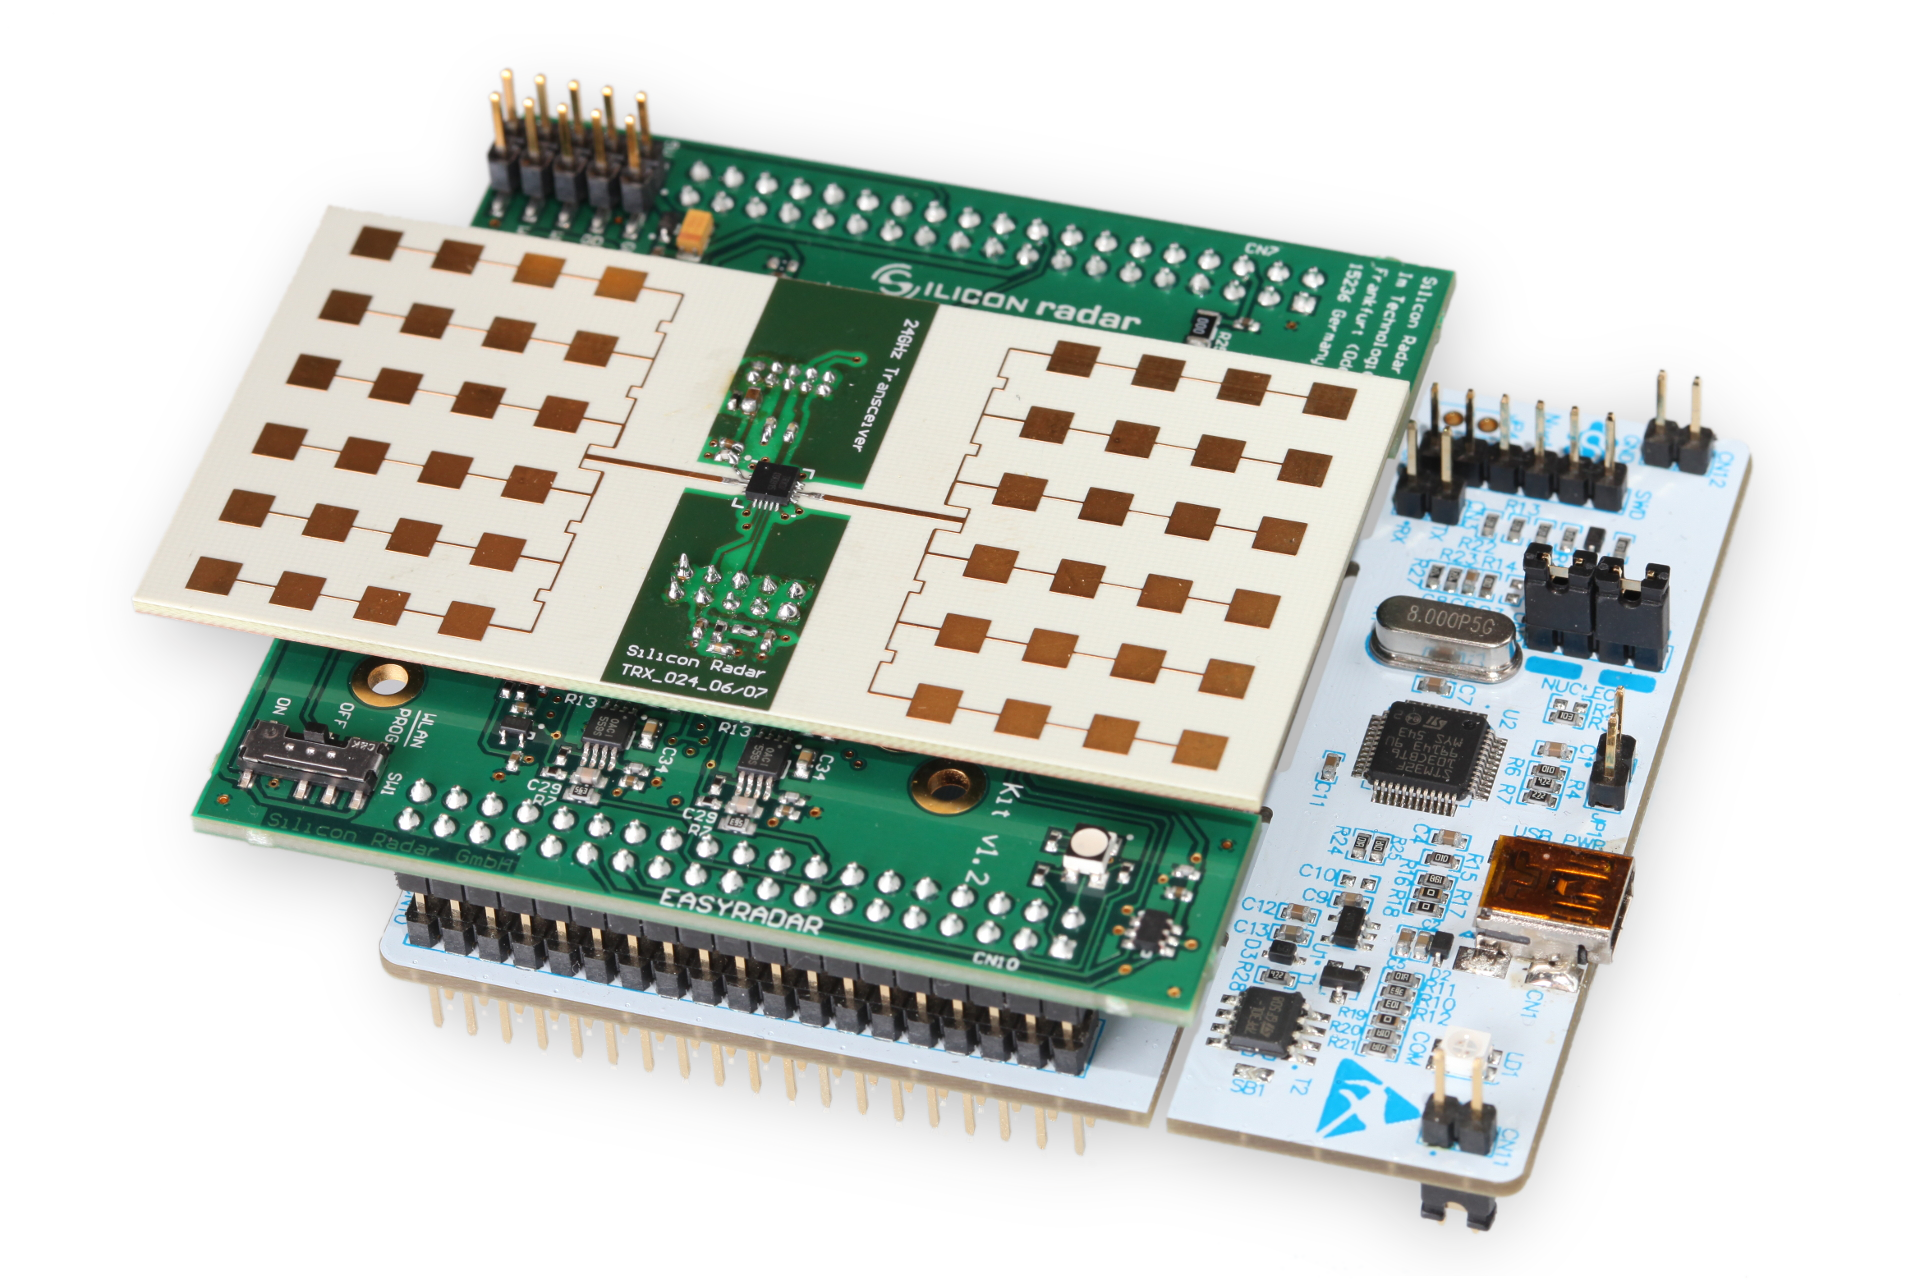
\includegraphics[width=0.6\textwidth]{../img/sirad.png}

  \caption[\sirad  24~GHz configuration \cite{siradMANOld}]{\sirad  24~GHz configuration \cite{siradMANOld}}
  \label{fig:sirad}
\end{figure}

Direct communication with the radar header is not possible, or at least, the communication interface is undocumented.
Instead, there is always an intermediary in the form of an STM32 Nucleo series microcontroller.
To this microcontroller, the user connects either directly with UART over USB or with WiFi, enabled by an on-board ESP32.
Both are relatively low-bandwidth communication methods, with the serial maxing out at a baud rate of 1,000,000 \cite{siradMAN}.

\begin{figure}[h!]
  \centering
  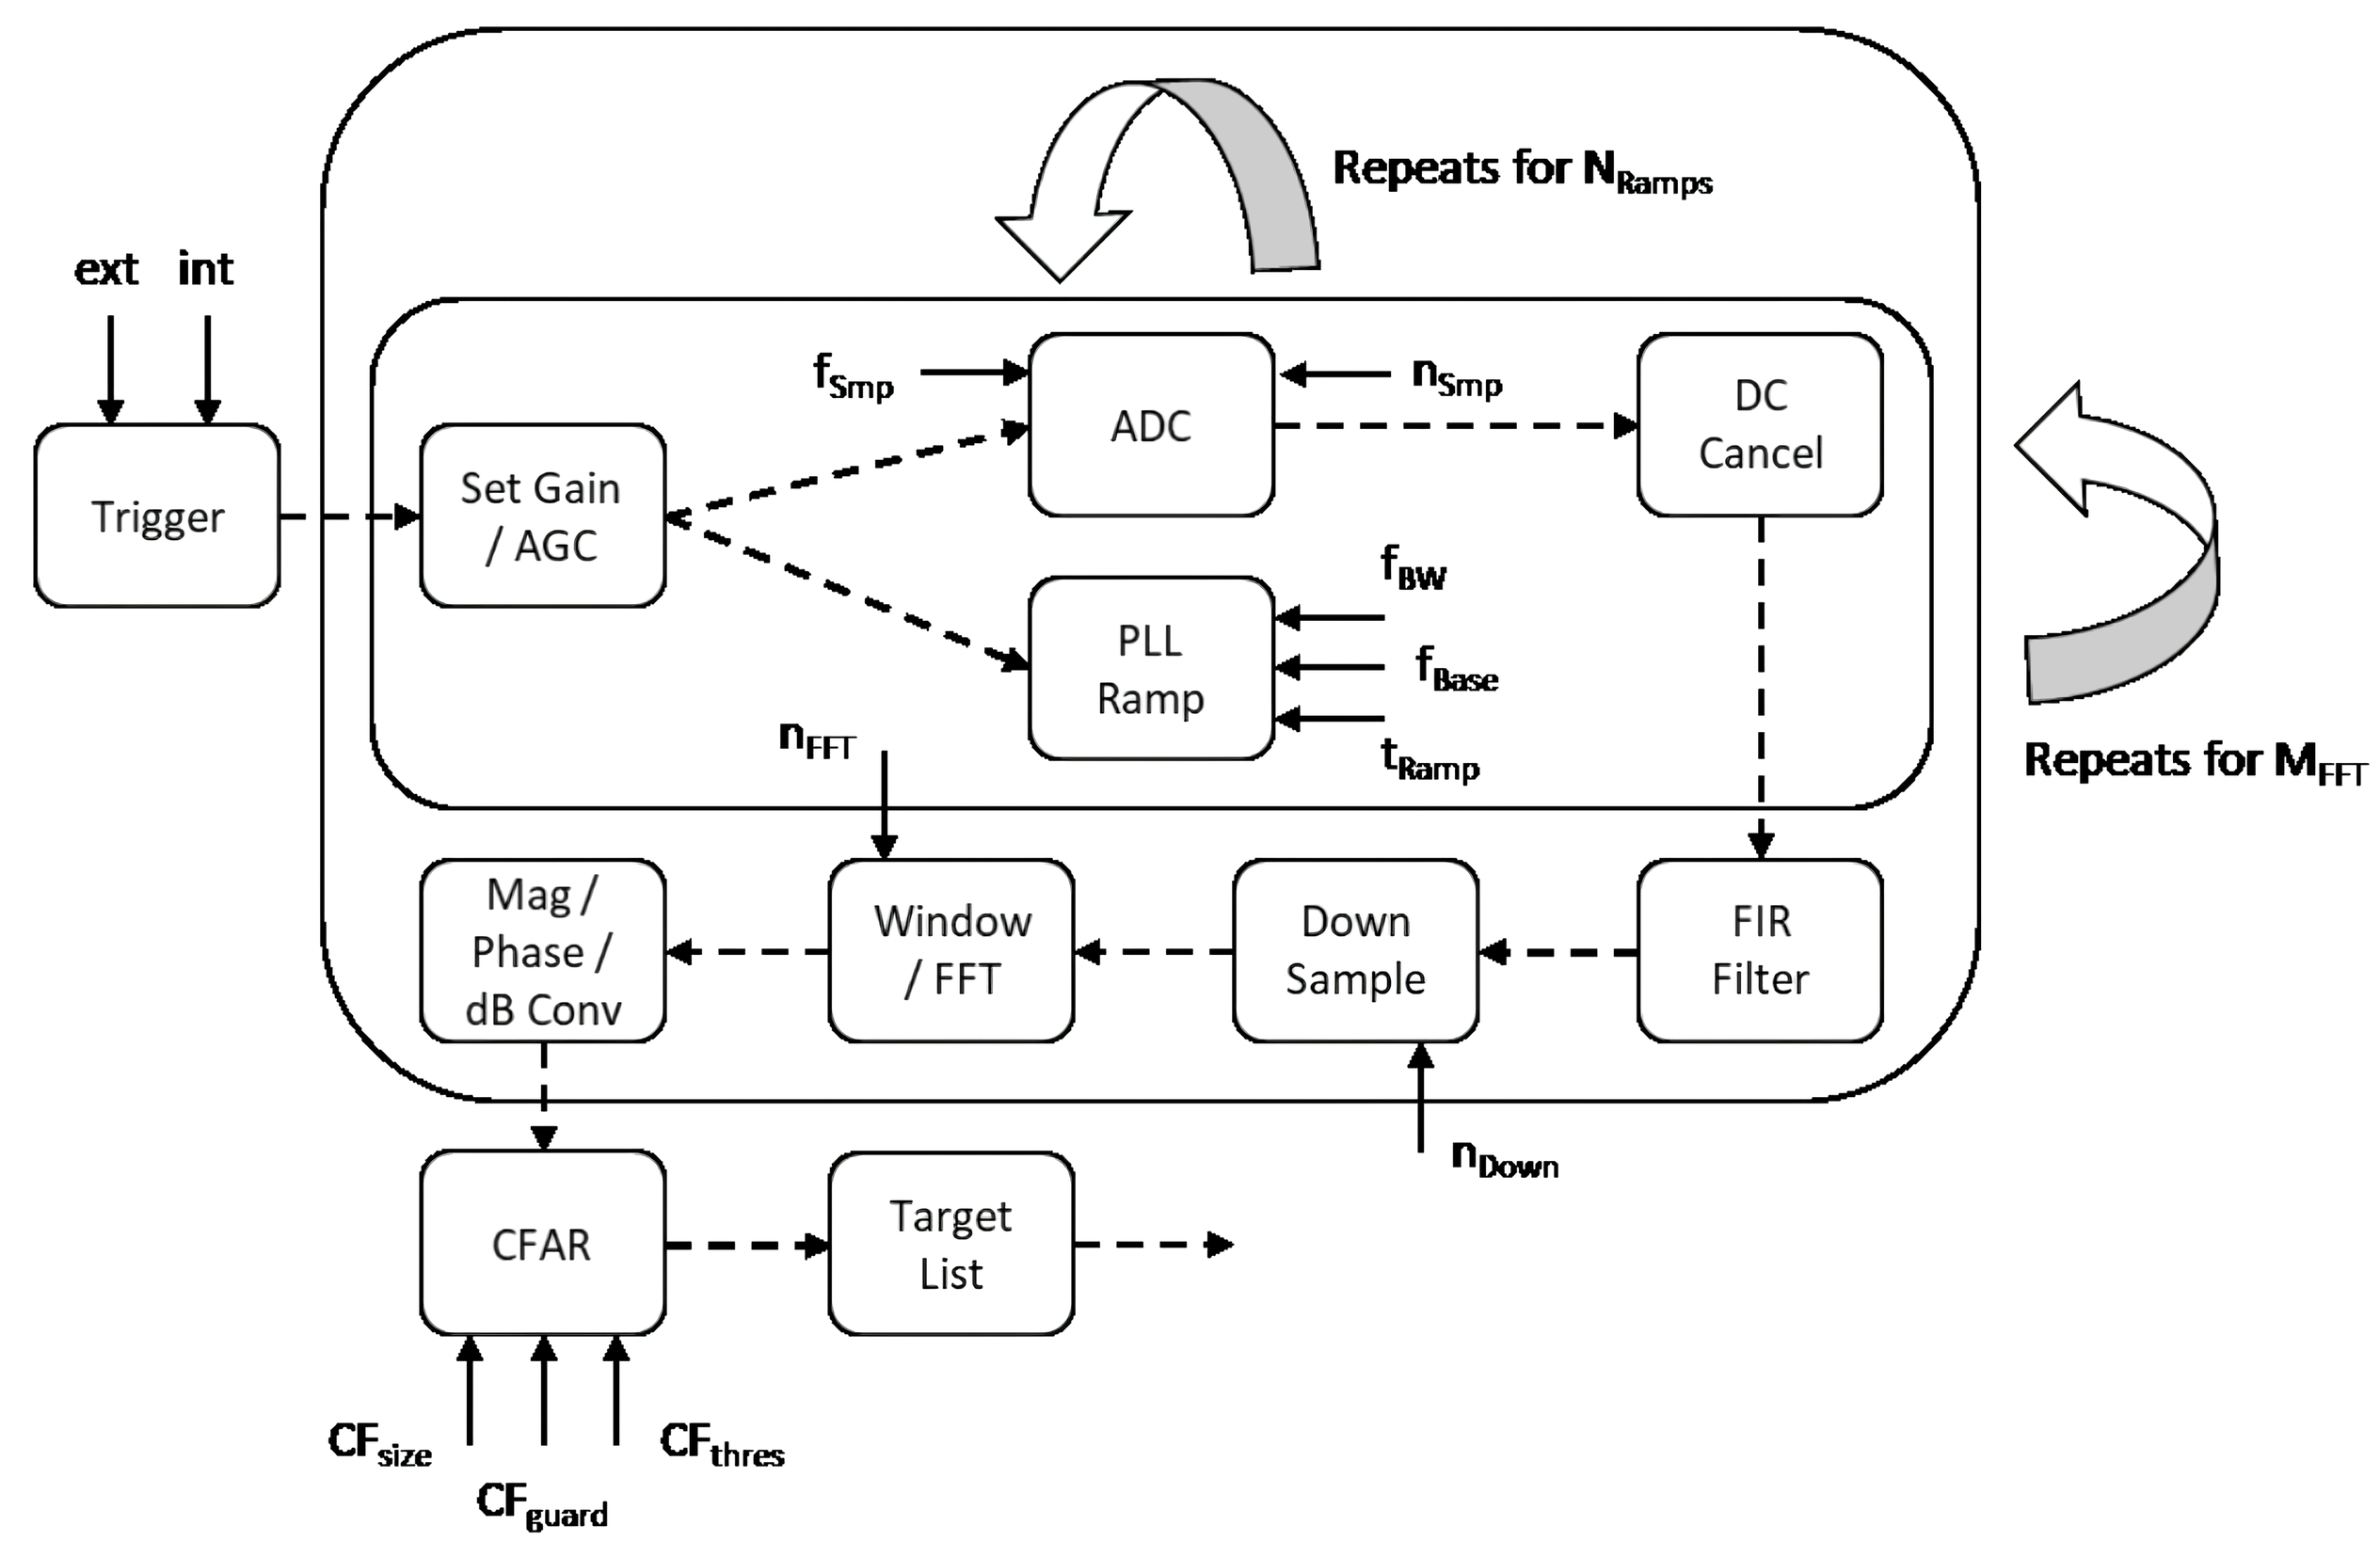
\includegraphics[width=0.7\textwidth]{../img/sirad_flow.png}
  \caption[Flow of Radar Measurement on \sirad \cite{siradPRO}]{Flow of Radar Measurement on \sirad \cite{siradPRO}}
  \label{fig:siradFlow}
\end{figure}

The devkit is designed for easy integration into existing projects; however, this unfortunately poses limitations for this thesis.
In normal operation, the radar system functions as a black box (processing schema shown in \ref{fig:siradFlow}), implementing its own filtering, FFT, and CFAR algorithms while only reporting a target list to the user.

This entire sequence started either by internal trigger or with external input (Be it via a GPIO pin or UART.).
Once the trigger is received, the device carries out a user-configured number of chirps.
Each with length determined by the number of sampling steps and the ADC sampling time as follows
\begin{equation}
  t_\mathrm{ramp} = \frac{t_\mathrm{ADC} \cdot  (N_\mathrm{samples} + 85)}{36\,\, \mathrm{MHz}} \,\, \mu\mathrm{s}.
  \label{eq:sampling}
\end{equation}
The manufacturer recommends keeping $r_\mathrm{ramp}$ around 1~ms for a good SNR \cite{siradPRO}.

SiRad is designed to leverage coherent averaging to improve SNR of the output.
This is achieved by broadcasting multiple ramps in series and averaging the results.
While this technique was found to aid in measurement in a cluttered environments averaging effectively destroys the information about the Doppler shift.
Additionally, due to the devkit's limited computational resources instead of a sawtooth waveform the radar broadcasts a segmented one with significant delays in between \cite{siradPRO}.

The devkit is clearly focused primarily on range measurement with little to no regard payed for speed calculation.
Not only are chirps spaced with large delays (at minimum some 20~ms) but the radar doesn't even maintain constant intervals between chirps.
This is the case even when relying on manual triggering of the radar.
When using radar's self trigger results are even worse.

When measuring reporting interval with 20~ms trigger the radar achieved average time between updates of 20.5~ms with standard deviation of 1.3~ms.
However from time to time they were outliers when report came in only after 30~ms in the worst case or just 16~ms in the best case.
This was on relatively small dataset of 5000 samples.
In order to rule out that the problem isn't only in reporting output signal from the radar was captured by Rohde \& Schwarz FSW26 Signal and Spectrum Analyzer.
By analyzing some 40 samples, broadcasted with the same trigger interval of 20~ms, average time between chirps was 20.7~ms with standard deviation of 0.7876~ms thus proving that broadcast itself is irregular.

Unfortunately as the radar doesn't maintain constant intervals between chirps speed measurement precision is severely limited.
This could be partially mitigated if we knew when the chirp was broadcasted, giving us ability to introduce a correction.
However no such information is provided by the radar.
Thus each chip is timestamped with it's time of arrival which is assumed to be the time of chirp broadcast.
Using this timing information speed spectrum can still be estimated using non-uniform DFT.

According to the radar's manual \cite{siradPRO}, the following equation was used to calculate the width of a single range bin:
\begin{equation}
  \Delta R = \frac{c_0 (N+85)}{2\cdot BW\cdot NFFT},
  \label{eq:rangeBin}
\end{equation}
where the variable $N$ denotes the number of samples and $NFFT$ the number of DFT points used to calculate the spectrum.
Except the corrective constant of 85 it closely follows the formula (\ref{eq:distance3}).

As for velocity the manufacturer doesn't recommend any formula so (\ref{eq:Doppler3}) was used with $T_\mathrm{ch}$ substituted by the user-chosen trigger period.
However, as the minimal period of chirps is rather high, not to mention the radar doesn't maintain constant intervals between chirps, the velocity measurement is not very practical.
Were we to use 24~GHz header with 25~ms trigger we get maximal speed of 0.124~m/s and on low 8 NFFT steps and the resolution is only $0.031$~ms$^{-1}$.

This lack of performance severely limits the radar's usability with regard to surveillance applications.
Most surveillance radars are designed to monitor dynamic environments, where targets are moving, usually at much higher speeds than the \sirad can measure.
This radar is completely unsuitable for such applications and is mainly applicable to static environments.
For example, in a parking lot, an operator can detect if a car is parked in a given spot or not.
However, besides such binary information about the presence of a target and its distance, not much more can be said.

\section{Outline of the Chosen Configuration }

For the purpose of this project, the devkit was configured to output raw data from the 12-bit ADC in the form of in-phase and quadrature components of the signal.
This allows for more complex processing than if the spectrum was calculated on the radar itself.
However it must be said that regardless of the output format the reported values are don't use the full 12-bit range, highest values reported were around $\pm 60$.

Given the unreliability of the radar's internal internal trigger the device was set up to be triggered externally.
In order to not complicate the system too much, trigger over serial line was used.

Another parameter to consider in relation to surveillance application was AGC.
Using it adds two additional ramps that are used solely to set the gain value, leading to some 3 ms delay.
However, a bigger problem is the fact that the radar doesn't report the gain value.
Using AGC could then lead to situations where the weighting of the data is not constant across rotation.
Thus, it was deemed safest to turn AGC off and set the gain manually, depending on how the readings appear after processing.

It is also important to note that the radar system is not well-suited for on-the-fly configuration changes.
Applying a new configuration takes some time, and the radar does not provide any feedback to indicate when a new configuration was applied.
As a result, commonly used techniques such as alternating chirp slope are not feasible.

In regard to the output format, the radar system supports two options: binary and TSV.
Since the output speed does not differ significantly between the two, the primary deciding factor was ease and speed of parsing.
Even when MATLAB is not particularly optimized for parsing binary data, it still processes binary output approximately 40\% faster than human-readable TSV data.

Other parameters, such as sampling frequency and the number of samples, were left to the user to configure.
Setting these strongly depends on which header is used and the environment in which the radar is in.
Thus, making their configuration static wouldn't be a good idea.


\section{24~GHz Header}

The core block of 24~GHz header is a SISO TRX-024-007 transceiver, which integrates low noise amplifier, frequency mixer, filters and VCO into a single package.
It is primarily designed to operate in the ISM band (24.0--24.25 GHz), but also supports an additional ultra-wideband mode with a frequency range from 23 GHz to 26 GHz \cite{siradTRX24}.
On the \sirad there is no distinction made between  those two modes and the user is free to set any bandwidth they want \cite{siradPRO}.
The transmitter output power ranges from 2.5 dBm to 6 dBm, depending on the configuration \cite{siradTRX24}.
A maximal range of 400 m is advertised \cite{siradMANOld}, though in practice only ranges of around 300~m were achieved, with target being a multistory building.

As shown in figure \ref{fig:sirad}, the chip is connected to two microstrip patch antennas.
The patches are arranged in a relatively standard configuration, forming a 6 $\times$ 4 array with spacing approximately equal to half the wavelength at 24 GHz.

Since the manufacturer did not provide any information about the radiation pattern of the array, a simulation was conducted using the CST simulation suite.
Additionally, the manufacturer did not disclose the substrate parameters for the radar board specifically.
Fortunately, the TRX-024-007 datasheet includes a board stack-up for the chip's evaluation board.
It was assumed that the same stack-up would be used: 18 \textmu m copper for the traces and ground plane, with a 250~\textmu m thick Rogers RO4350B substrate \cite{siradTRX24}.

\begin{figure}[ht!]
  \centering
  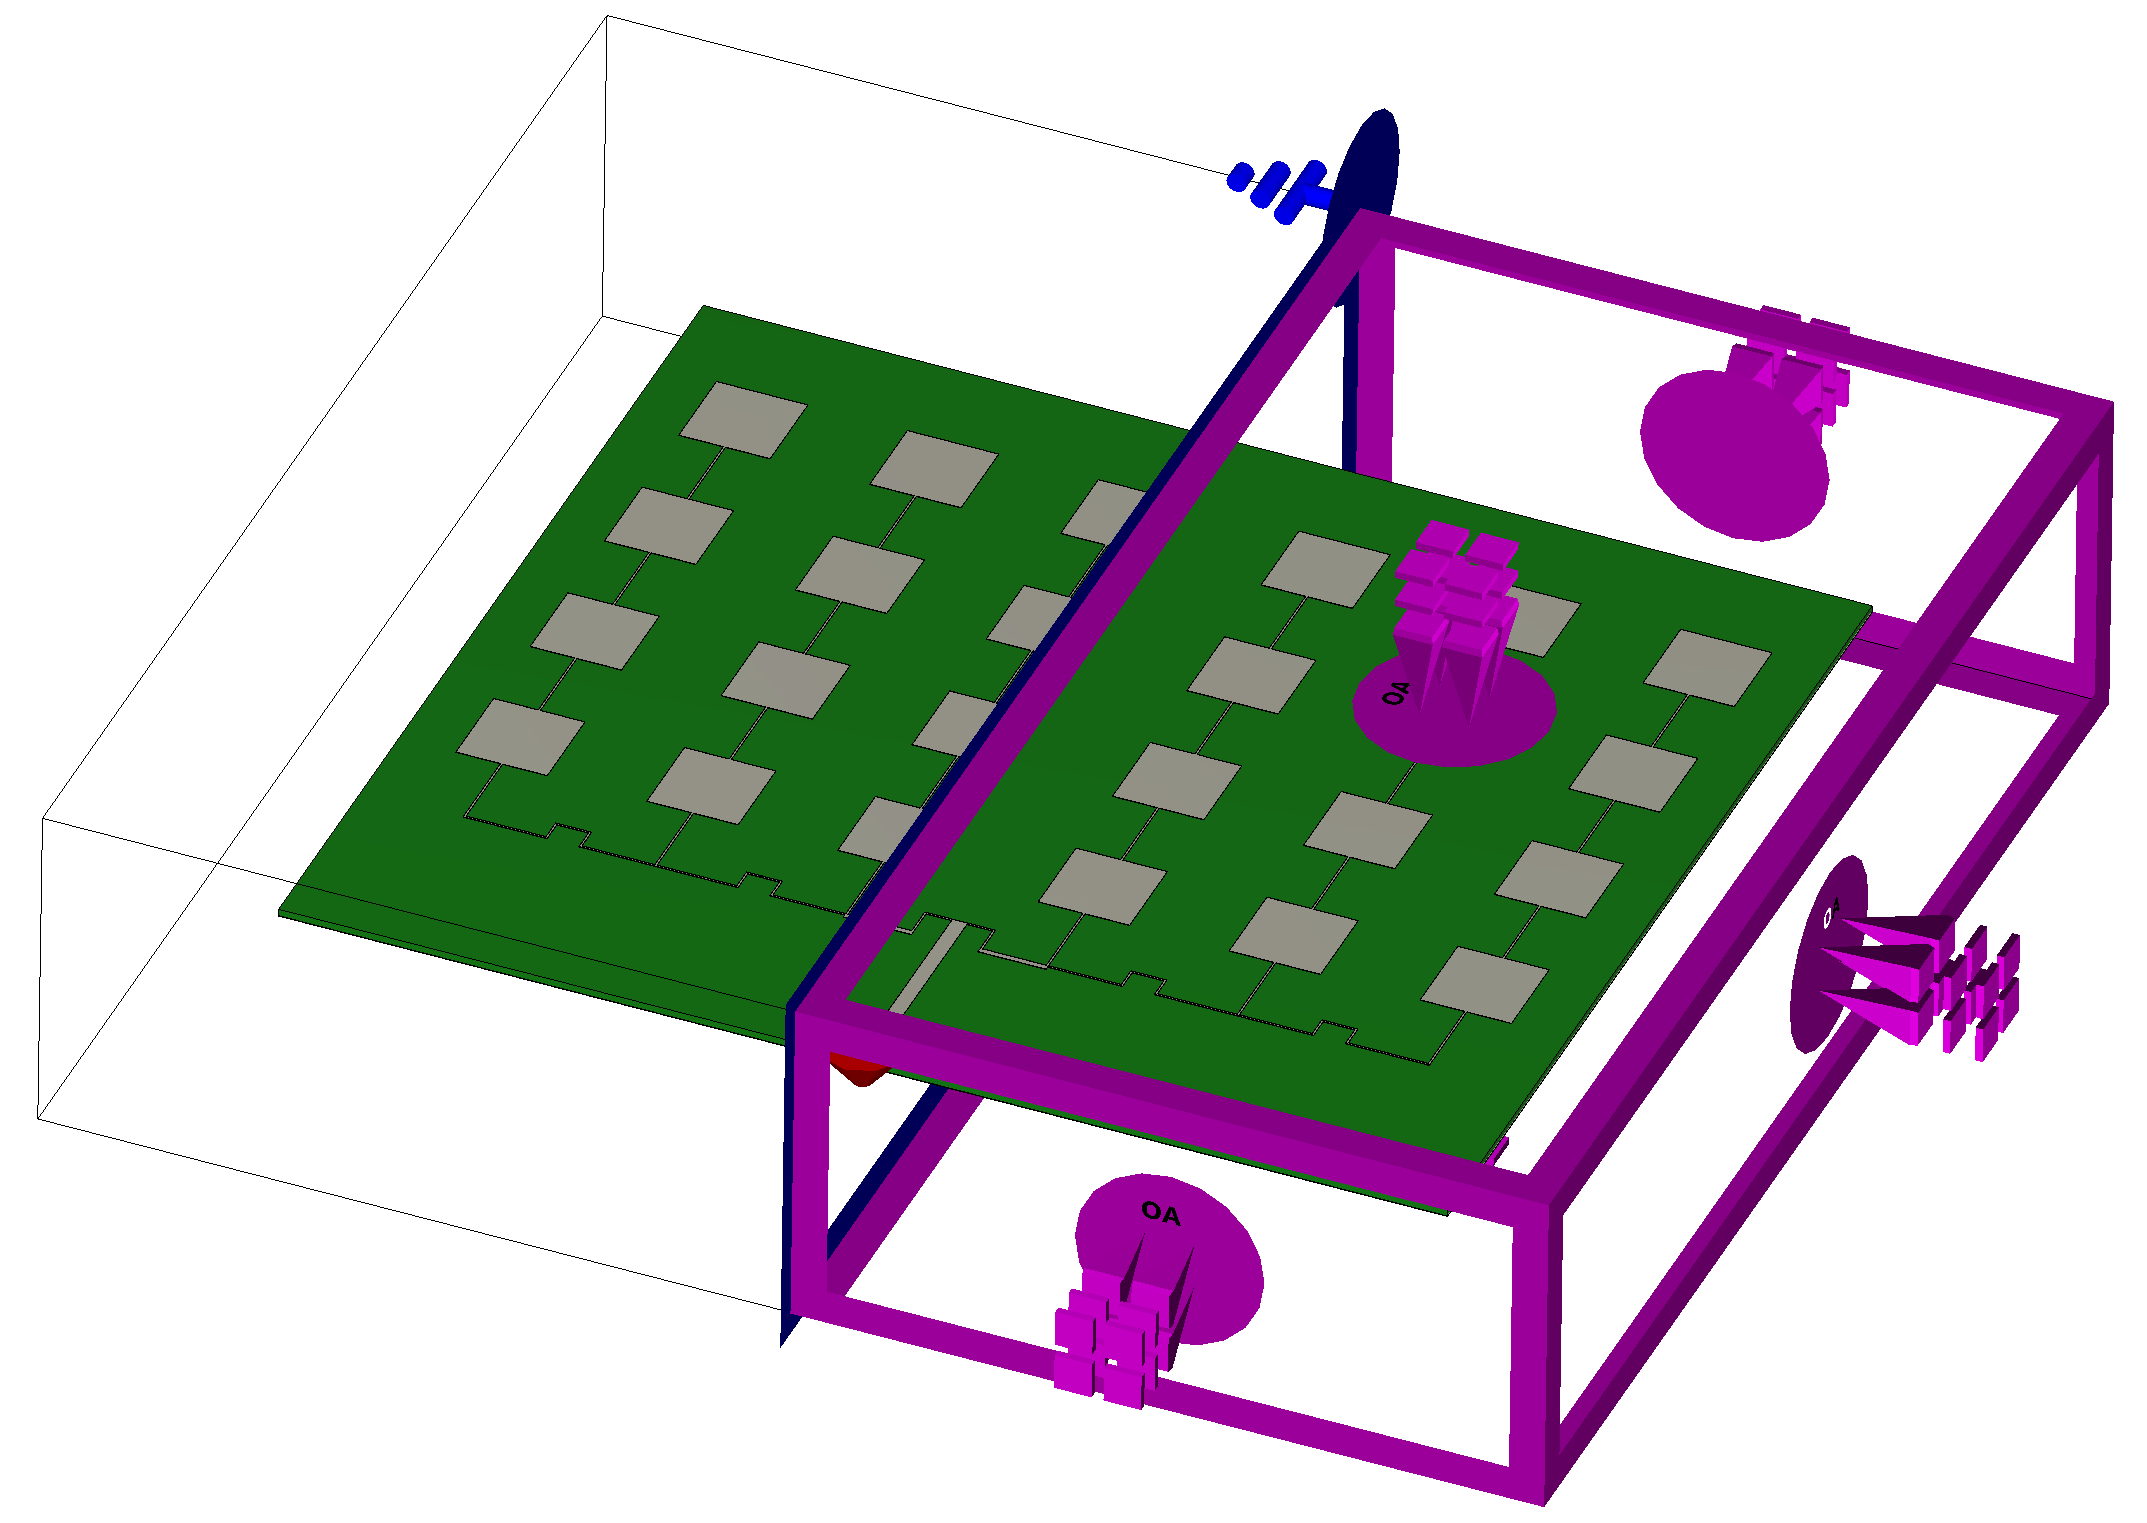
\includegraphics[width=0.6\textwidth]{../img/boundaries.png}
  \caption[Simulated 24 GHz header with boundary conditions showed]{Simulated 24 GHz header with boundary conditions showed}
  \label{fig:boundaries}
\end{figure}

After measuring the dimensions of the array using an optical microscope, the entire array was redrawn in CST Studio.
Figure \ref{fig:boundaries} shows the applied boundary conditions: the antenna was placed in open space, and a  $H_\mathrm{norm}=0$ condition was set along the symmetry plane to speed up the simulation.

After performing a standard time-domain simulation with an excitation signal ranging from 0 to 26GHz, the antenna array exhibited a minimum reflection coefficient $s_{11} \doteq -26.4 \mathrm{~dB}$ at 23.478~GHz with second minimum at 24.518~GHz (Figure \ref{fig:s11}).
The lack of minimum at 24~GHz is likely due neglecting imperfection in the manufacturing process where roughness of the copper traces manifests as a change in the effective dielectric constant of the substrate.

At both frequencies with minimal reflection, a far-field radiation pattern was calculated.
For clarity, only the 24.518~GHz pattern is shown in figure \ref{fig:farfield3d}.
The main lobe width was measured at approximately 16 degrees (Figure \ref{fig:farfield180}) along the 180-degree norm (for orientation refer to the red cone on the PCB visualization), with a peak gain of 18.6~dBi and side-lobe suppression of -13~dB.
For the 90-degree norm, the main lobe width (Figure \ref{fig:farfield90}) was 30 degrees, with side-lobe suppression of -10~dB.

It's clear that, especially in the 90-degree norm, the beam isn't that narrow.
Thus, this header is not suitable for applications where accurate elevation information is needed.
However, if only a low degree of accuracy is required or a wider field of view would be beneficial, this header is a good choice.
With wider beam  the radar can gather more information about the environment faster compared to one with a narrower beam.
In industry, some surveillance radars are also designed to have a wide beam in elevation, such as some Air Traffic Control radars \cite{kratos} or even some ground radars \cite{blighter}.
Still, usually, solutions such as low/high beam switching are preferred instead of relying purely on a wide beam \cite{wolfBeam}.

\begin{figure}[h!]
  \centering
  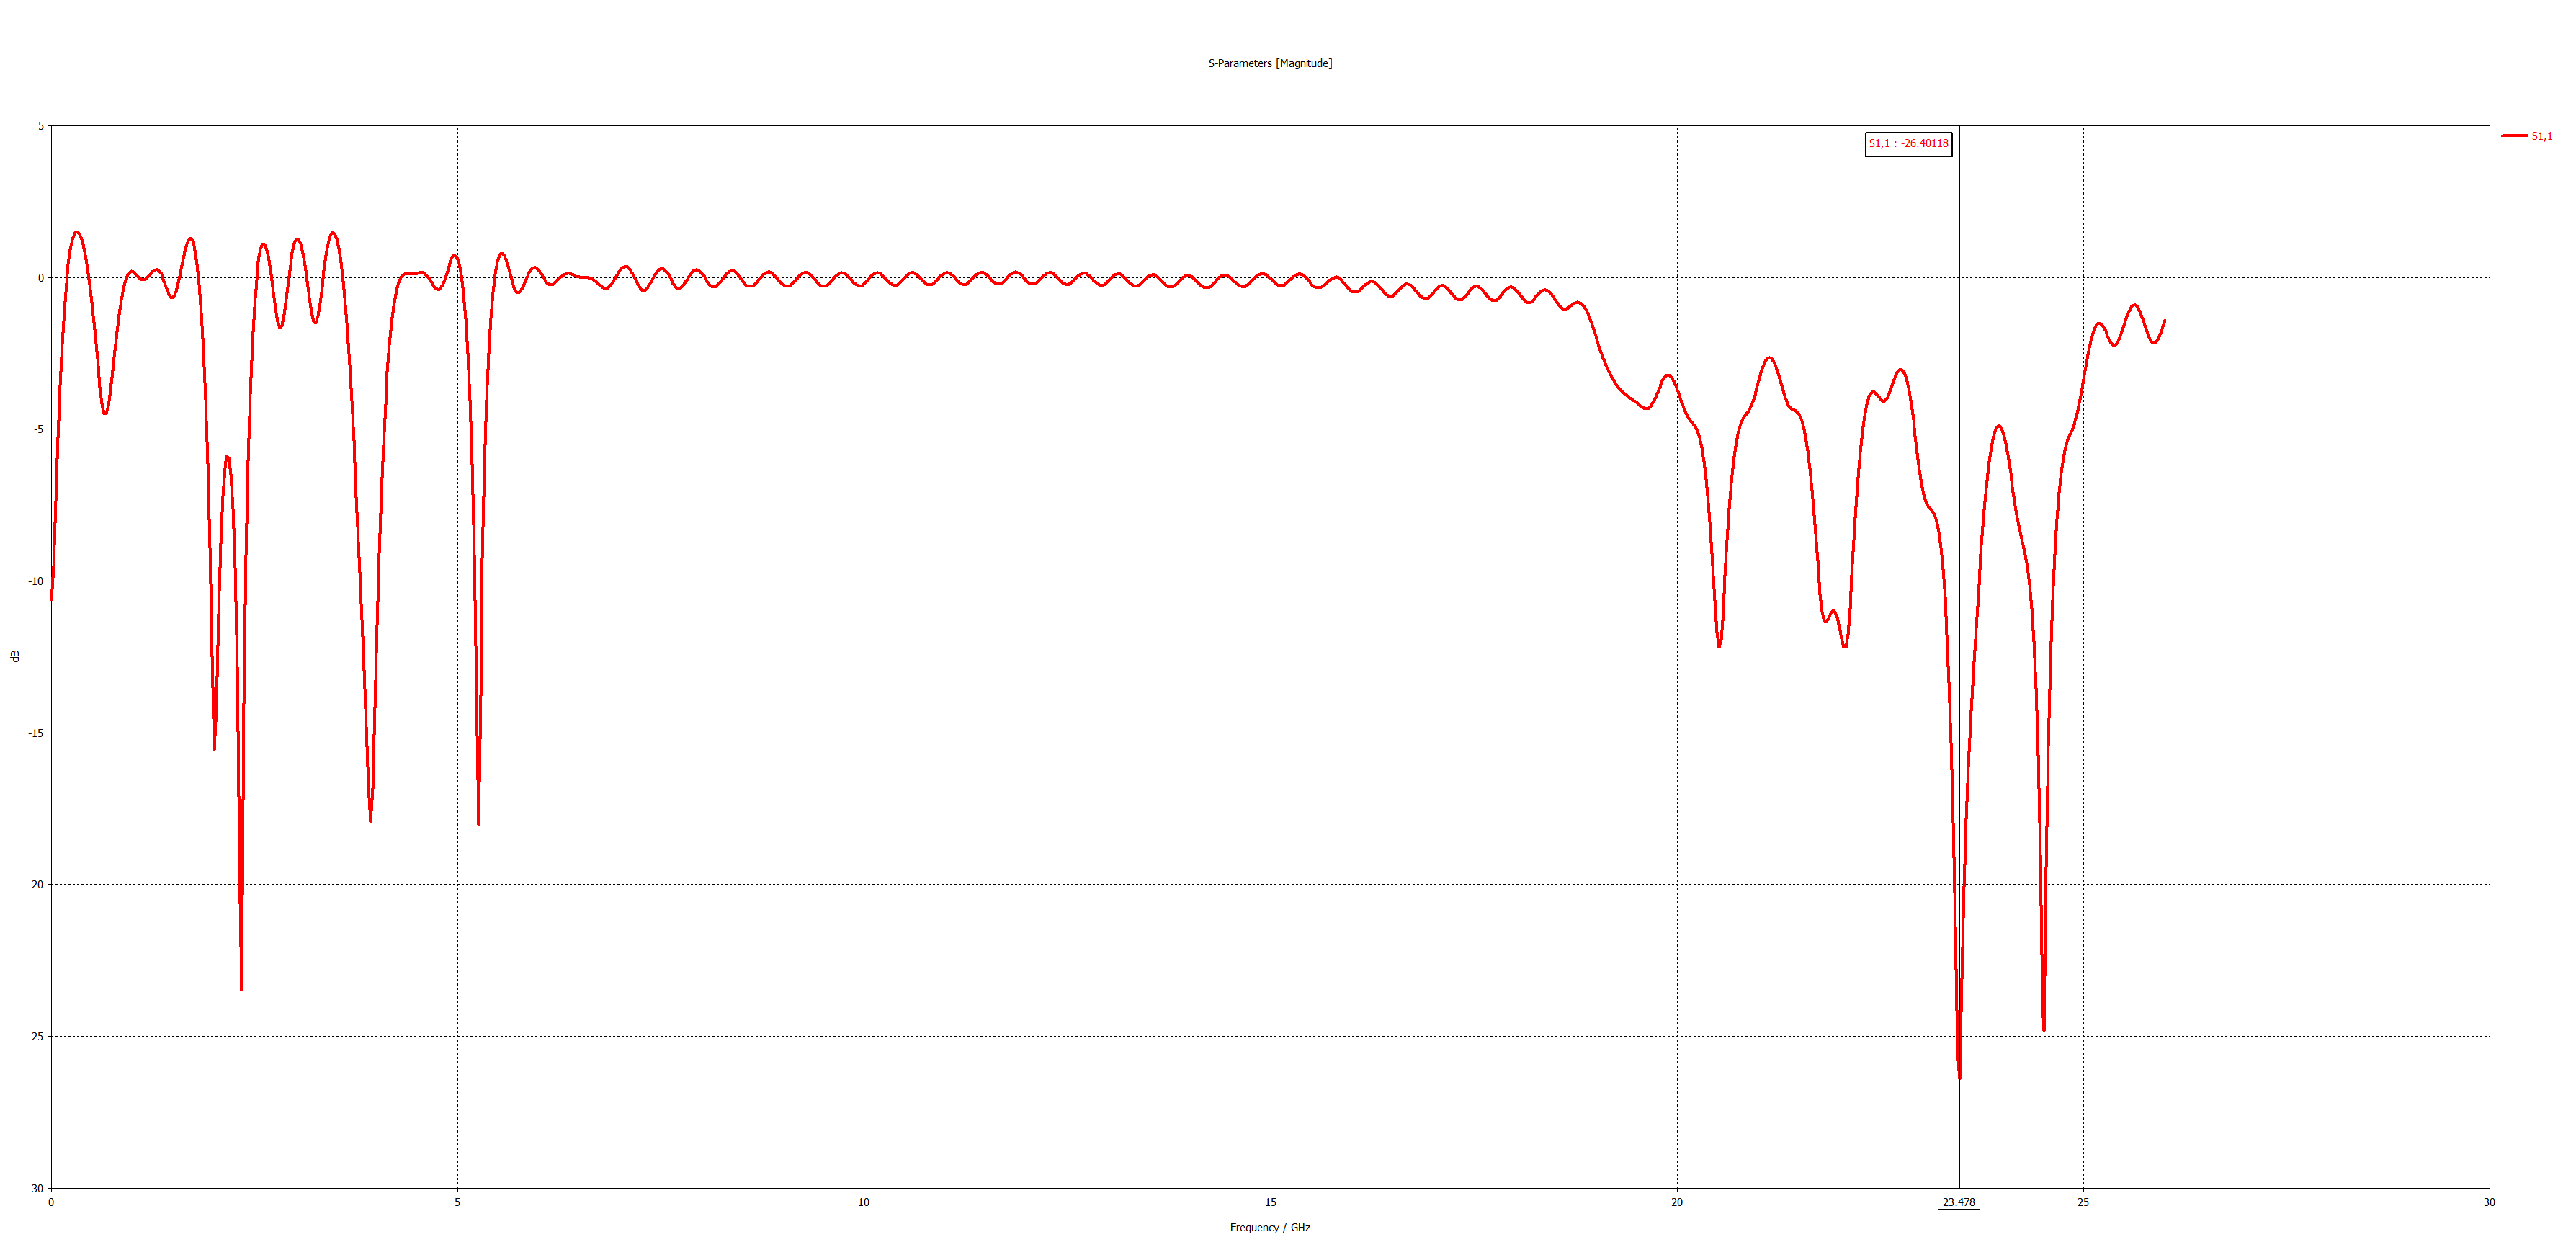
\includegraphics[width=\textwidth]{../img/s11.png}
  \caption[$s_{11}$ parameter of the 24~GHz header]{$s_{11}$ parameter of the 24~GHz header}
  \label{fig:s11}
\end{figure}


\begin{figure}[h!]
  \centering
  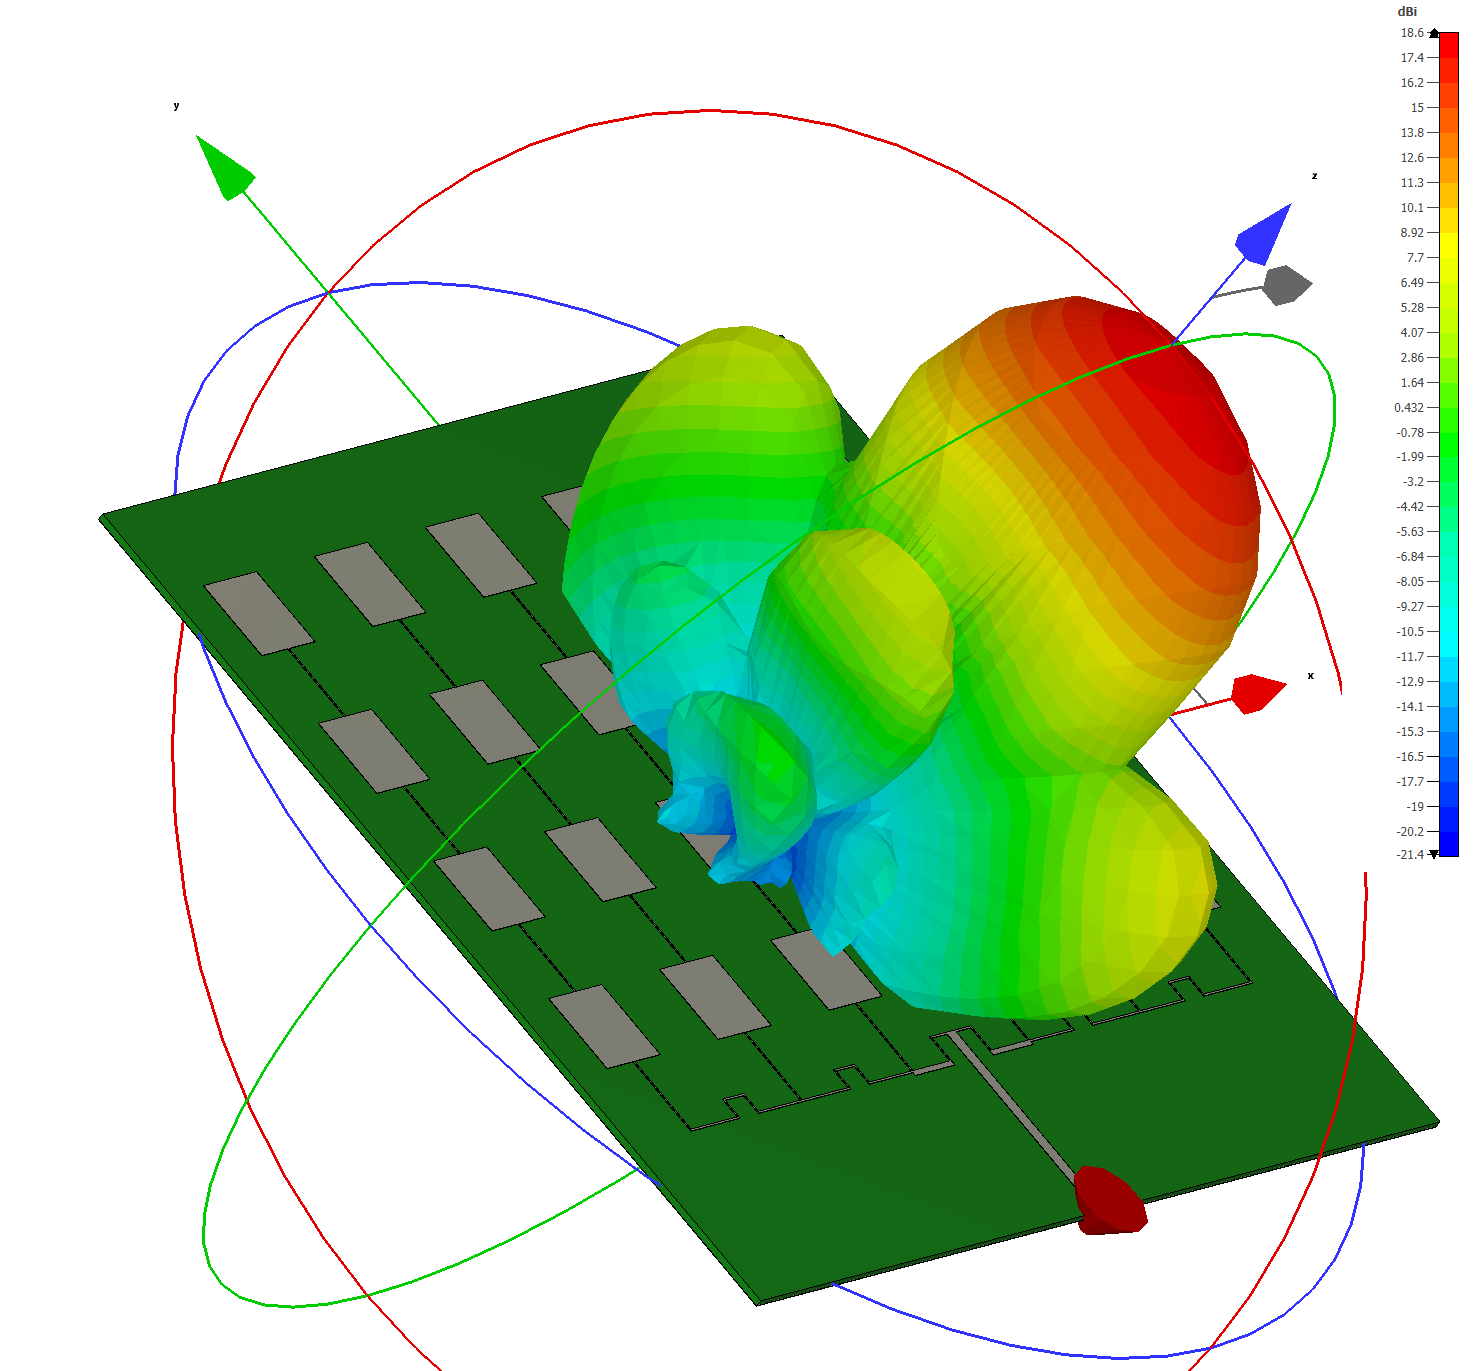
\includegraphics[width=0.43\textwidth]{../img/farfield3d.png}
  \caption[Radiation pattern of 24~GHz header -- 3D view]{Radiation pattern of 24~GHz header -- 3D view}
  \label{fig:farfield3d}
\end{figure}

\begin{figure}[h!]
  \centering
  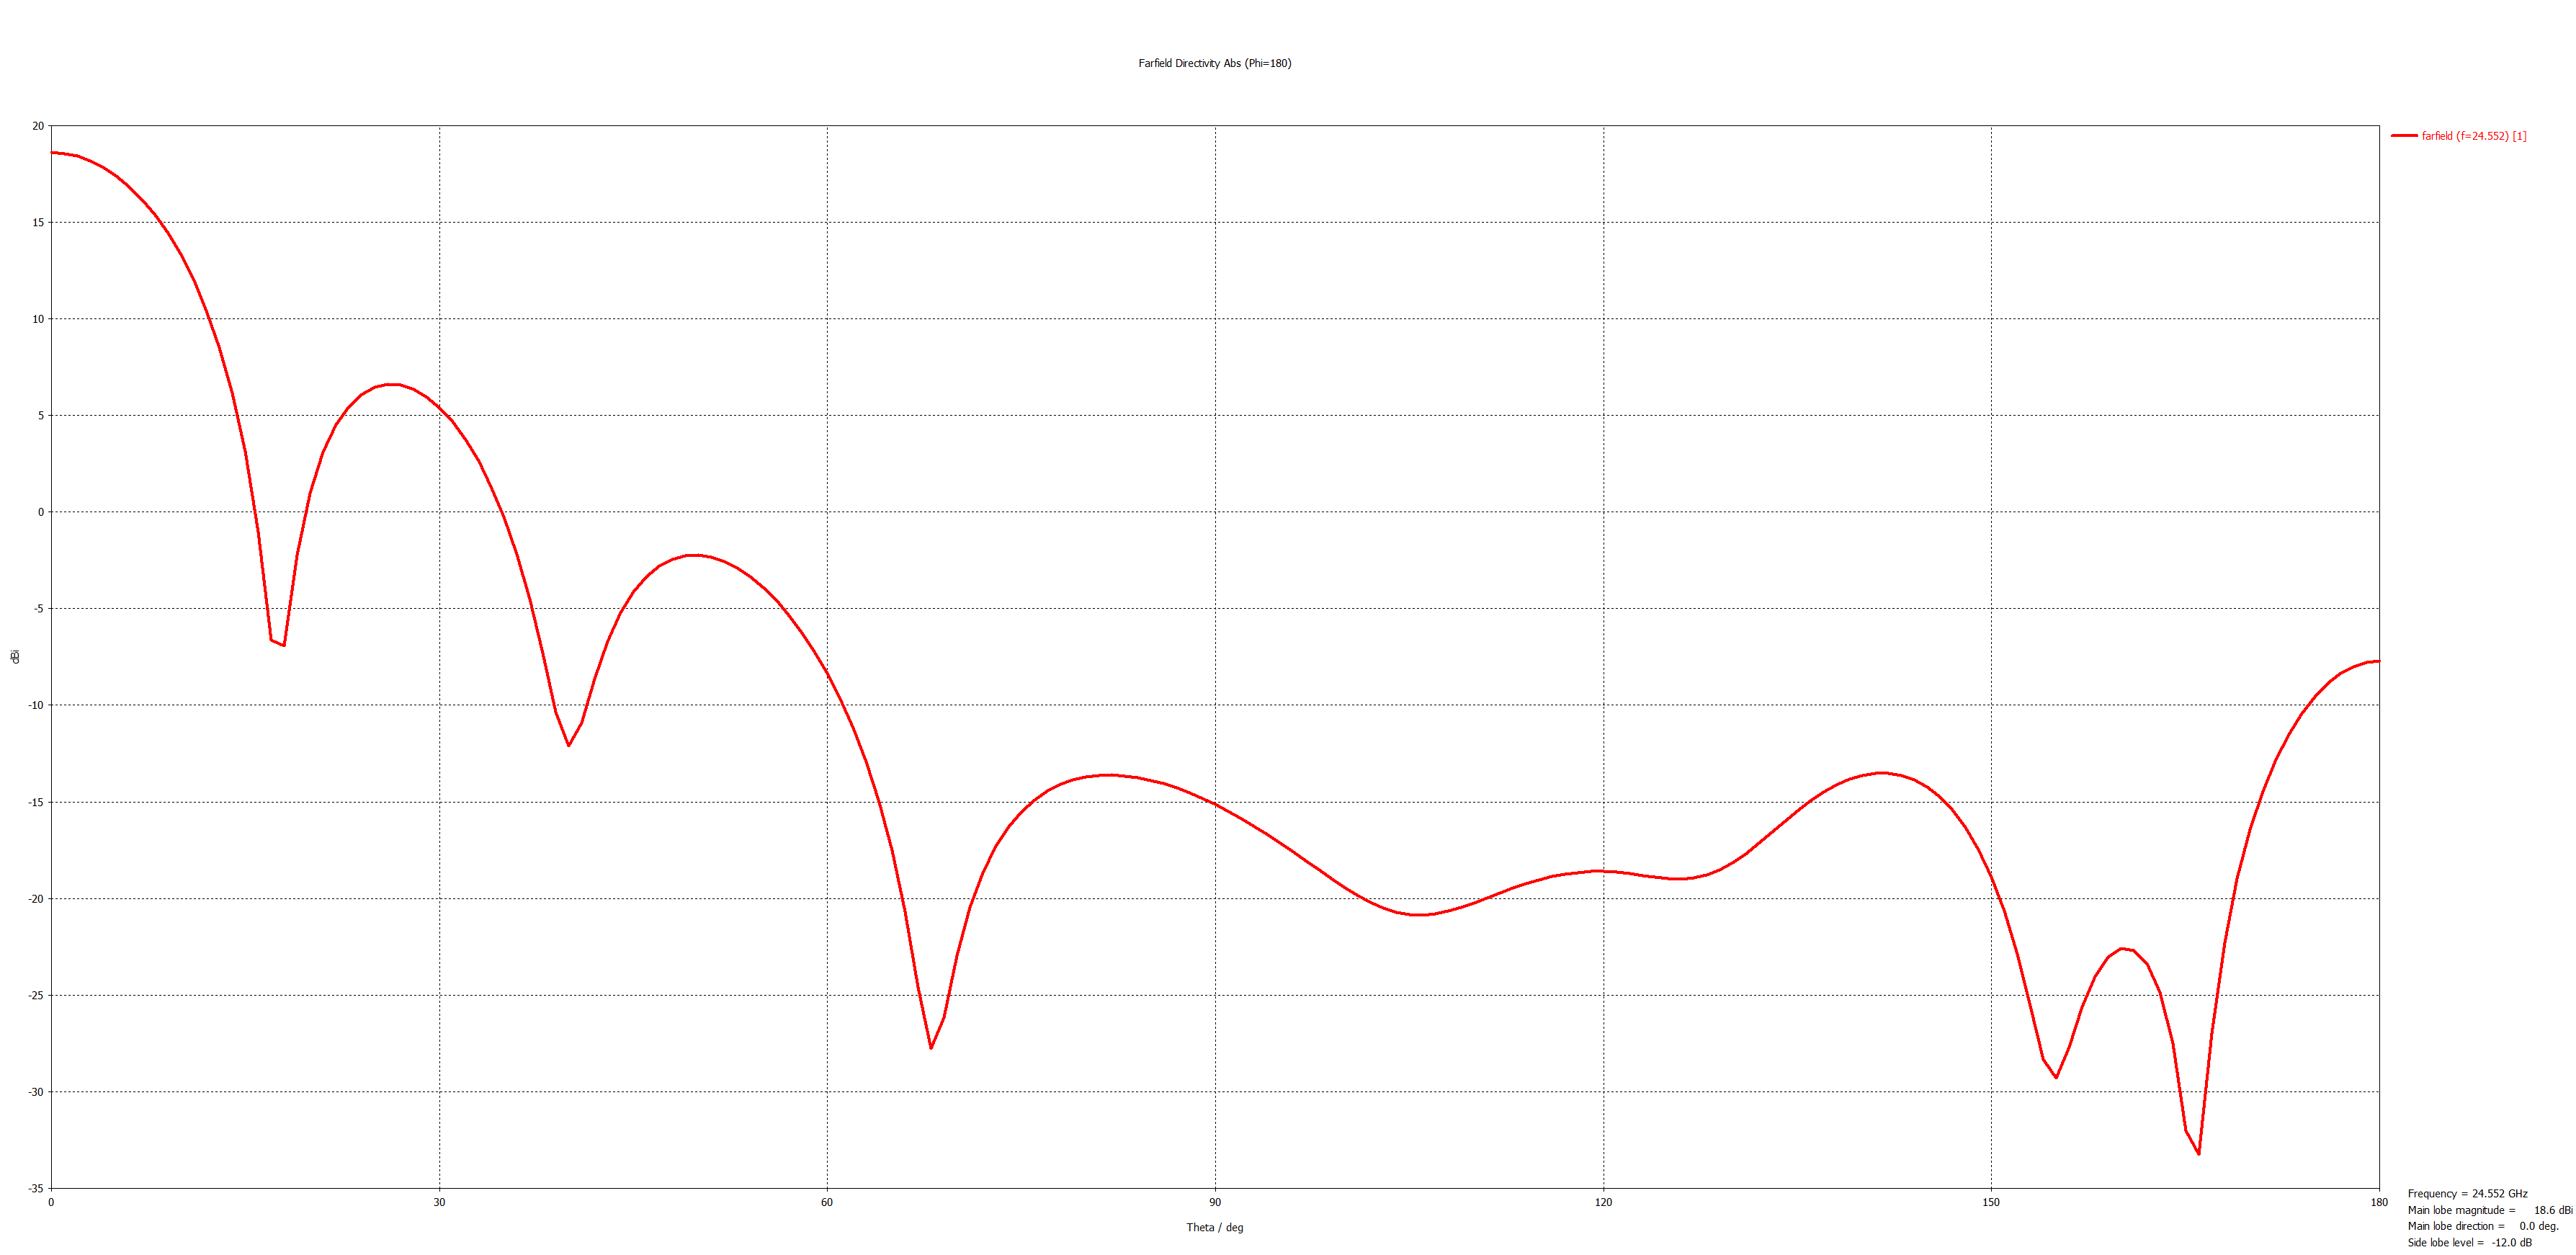
\includegraphics[width=\textwidth]{../img/farfield180.png}
  \caption[Radiation pattern of 24~GHz header -- 180° norm]{Radiation pattern of 24~GHz header -- 180° norm}
  \label{fig:farfield180}
\end{figure}

\begin{figure}[h!]
  \centering
  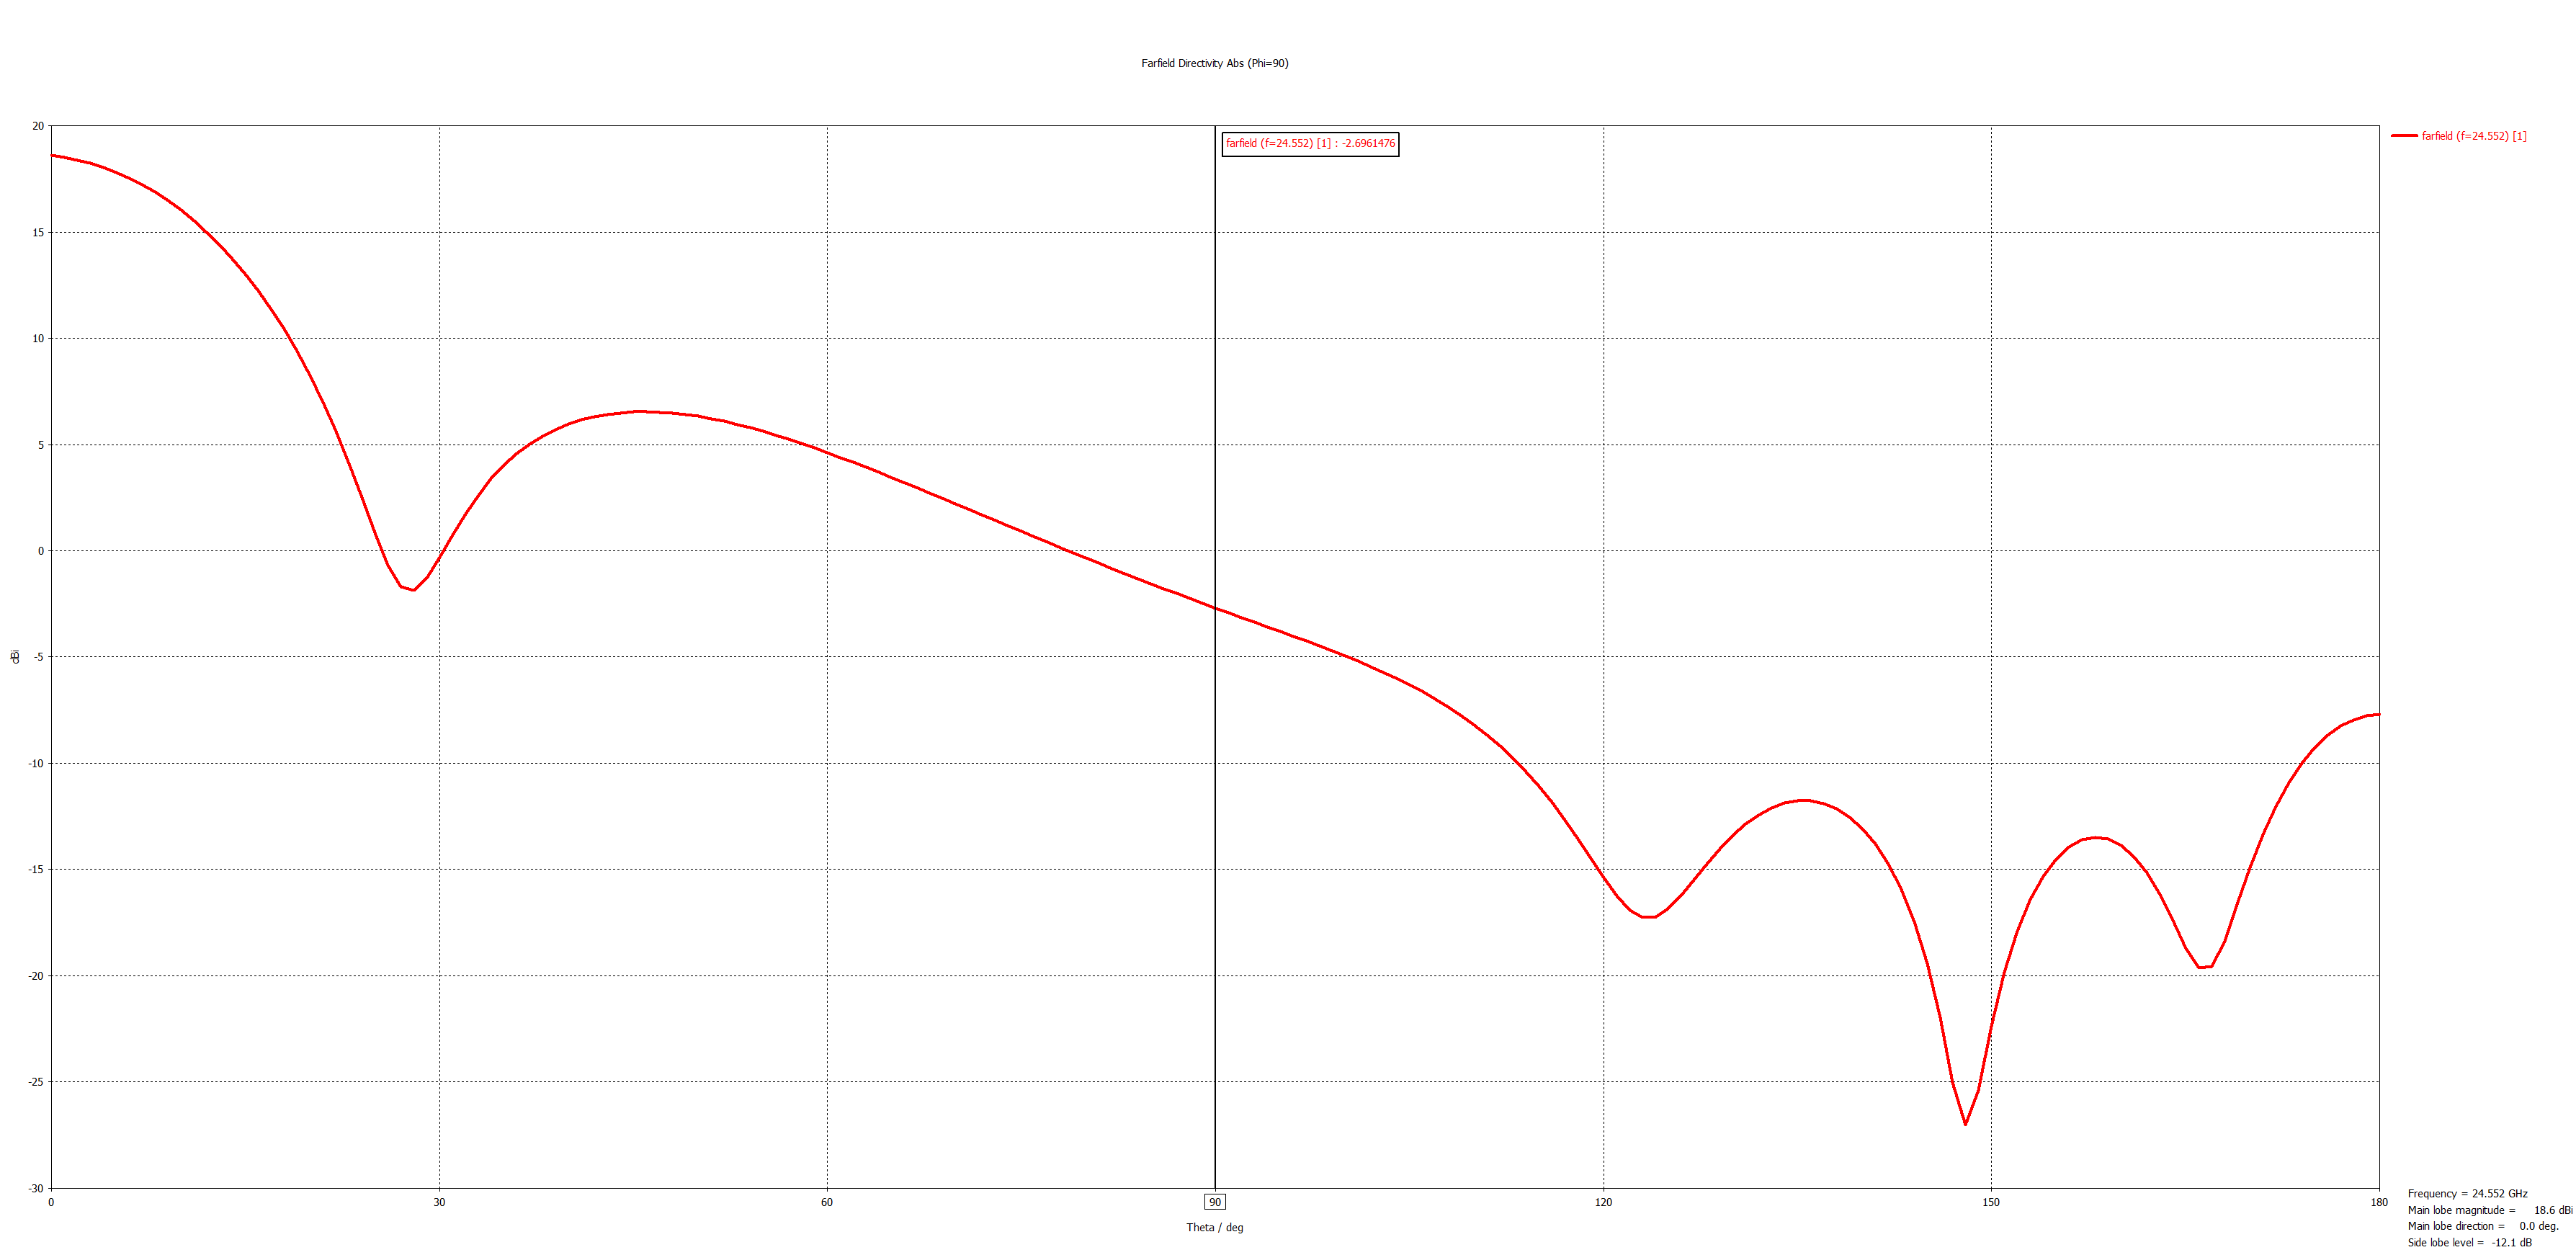
\includegraphics[width=\textwidth]{../img/farfield90.png}
  \caption[Radiation pattern of 24~GHz header -- 90° norm]{Radiation pattern of 24~GHz header -- 90° norm}
  \label{fig:farfield90}
\end{figure}


\section{122~GHz Header}


\begin{figure}[h!]
  \centering
  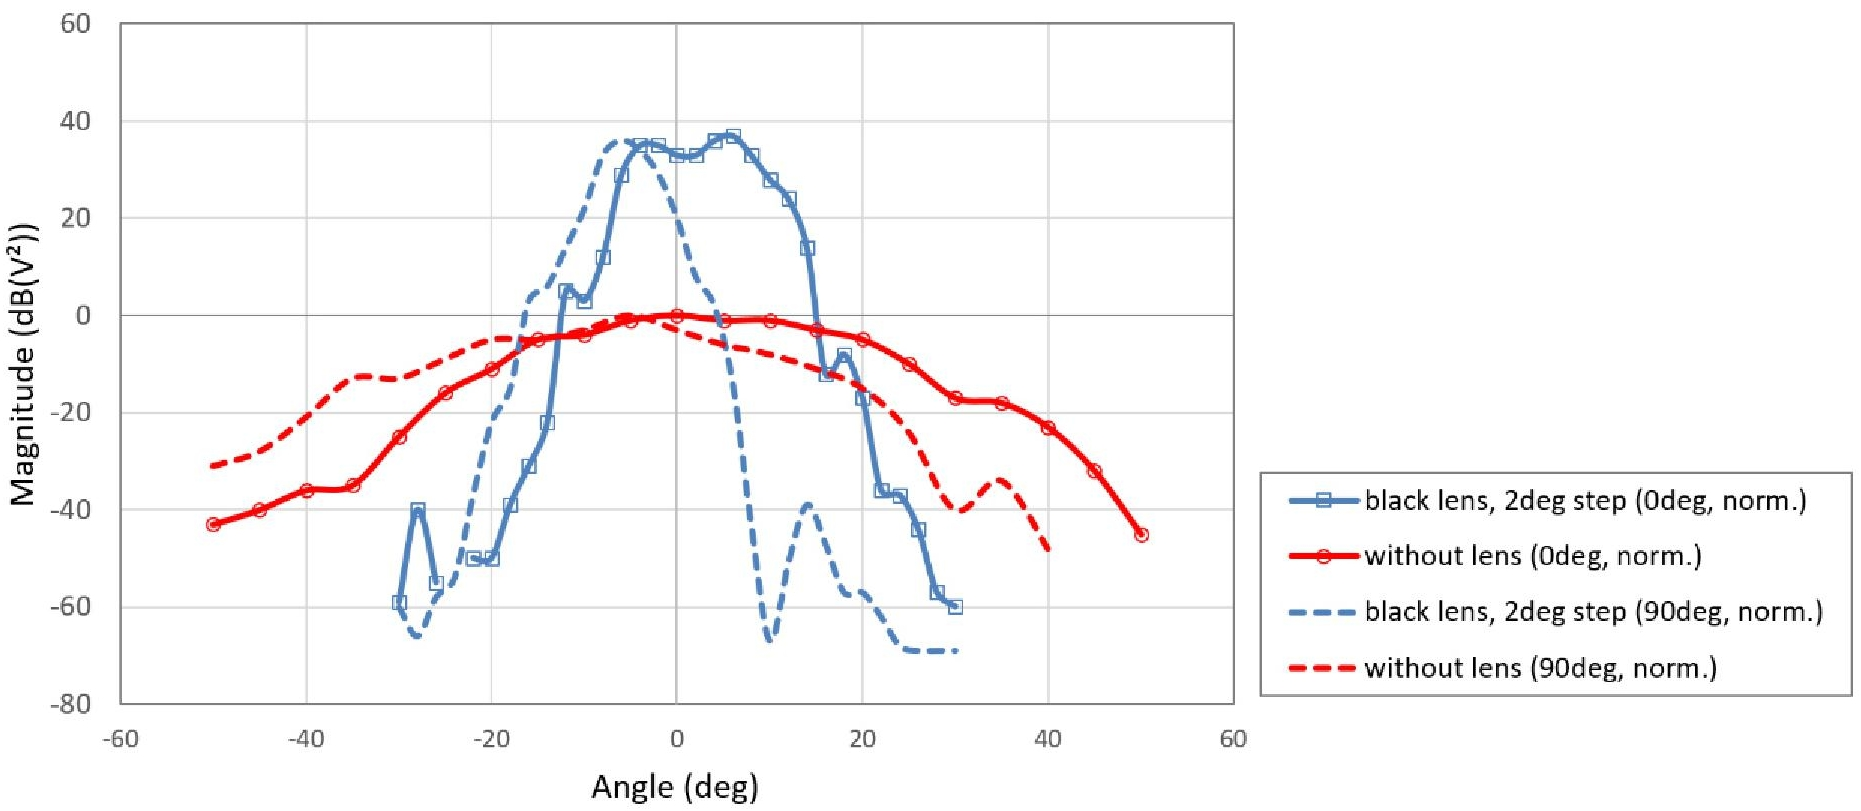
\includegraphics[width=0.85\textwidth]{../img/sirad122rad.jpg}
	\caption[Radiation pattern of 122~GHz header comparison \cite{siradTRX122col}]{Radiation pattern of 122~GHz header comparison \cite{siradTRX122col}}
  \label{fig:sirad122rad}
\end{figure}

The 122~GHz header is based on the TRX-120-001 transceiver, which, in addition to the essential components required for RF transmission and reception, also incorporates two on-chip antennas.
It's designed to operate in the 122-123~GHz band, with an output power ranging from -7~dBm to 1~dBm \cite{siradTRX122}.
The chip is advertised as capable of detecting large targets at distances of up to 40~m \cite{siradMANOld}.

Out of the box performance of the system is quite bad (Figure \ref{fig:sirad122rad}) with the width of the main lobe being roughly $\pm40\text{°}$ in both E-plane and H-plane \cite{siradTRX122}.
However, this can be significantly improved using the supplied collimator lens, reducing the main lobe width to $\pm4\text{°}$ \cite{siradTRX122col} (Figure \ref{fig:sirad122rad}).



\chapter{Rotary Platform}

The following chapter outlines the design process and operational principles of a rotary platform specifically developed for the \sirad radar system.


\section{Platform Construction}

As the platform needs to transmit data from the rotating section to the stationary base a slip ring is required.
Due to the relatively low transmission speed of the radar and the absence of special requirements such as waterproofing, an affordable model, UH3899-01-0810 from Senring, was selected.
It is a classic contact slip ring that features a dedicated USB~2.0 connection along with 8 additional signal wires.
Advertised insertion is less than 2~dB \cite{slipring}.
More problematic than the loss, however, is crosstalk between signal wires when the pitch control stepper motor is running.
This necessitated the addition of a small capacitor to the endstop signal wire to filter out high-frequency noise.

While the USB~2.0 connection does not seem affected by the crosstalk, its connection still isn't ideal.
Without a signal conditioner connected directly to the slip ring output, signal quality is poor enough that a direct connection to the PC is required -- thus, the radar needs to be some 20~cm from the PC.
Even then, depending on the PC's USB port wiring, some ports might exhibit issues.
In addition, the manufacturer opted for a non-standard male-male USB~2.0 connection, requiring a female-female adapter to connect the radar to the slip ring.

Due to the relatively low angular resolution of the radar, high platform precision was not a requirement.
A basic 200-step stepper motor with a step size of 1.8\text{°} was deemed sufficient.
In case the user requires more granular control over the position, it can be facilitated by microstepping.

Similarly, high-speed movement was unnecessary for this application.
As was already outlined, the radar is capable at best of some 50~Hz update rate.
To put things into perspective at low 8~RPM a degree of angle is traversed in 21~ms, thus any faster speed would lead to having less then one sample per degree.
At these speeds, standard 40~mm NEMA17 stepper motors were found to be sufficient.
However if faster rotation would be needed a stronger motor would be required as due to slipring stiffness the motor is already working at its limits.

The rest of the design is relatively simple.
Slipring is mounted to a 3D printed base that elevates it slightly above ground.
Stepper motor is then mounted directly under the slip ring, with a shaft connecting it to the rotating base.
The connection is secured using long M4 set screws that pass through the base, through the slip ring, and hold the shaft in place.
A 3D-printed housing serves only as a centering guide and is not under any load from the shaft connection.

The rotating section features a simple A-frame design that elevates the radar, which is mounted on two ball bearings, allowing it to tilt freely.
To control the pitch, a second stepper motor is mounted on the rotating platform and linked to the radar via a 2:1 down-gearing ratio using a standard 8~mm belt.
An optical endstop, used for homing the platform, is attached to the second support strut.

Unfortunately, while the design offers some ability to tension the belt, in the currently printed configuration the adjustment range is not sufficient to fully tension the belt.
While slippage is not a problem, there is some slack in the radar's tilt.
However, as the radar's capabilities in the pitch direction are not particularly high, it was decided not to reprint the whole assembly, but only to fix the issue in supplied 3D models.

Given that mechanical stresses are minimal, most parts can be 3D-printed using standard PLA filament.
The only non-3D-printed components are the screws, shaft, bearings and stepper motors.
The final assembly (Figure~\ref{fig:side_by_side}) measures approximately 36~cm in height and has a footprint of roughly $20\times20$~cm.

\begin{figure}[h!]
  \centering
  \begin{subfigure}[b]{0.55\textwidth}
    \centering
    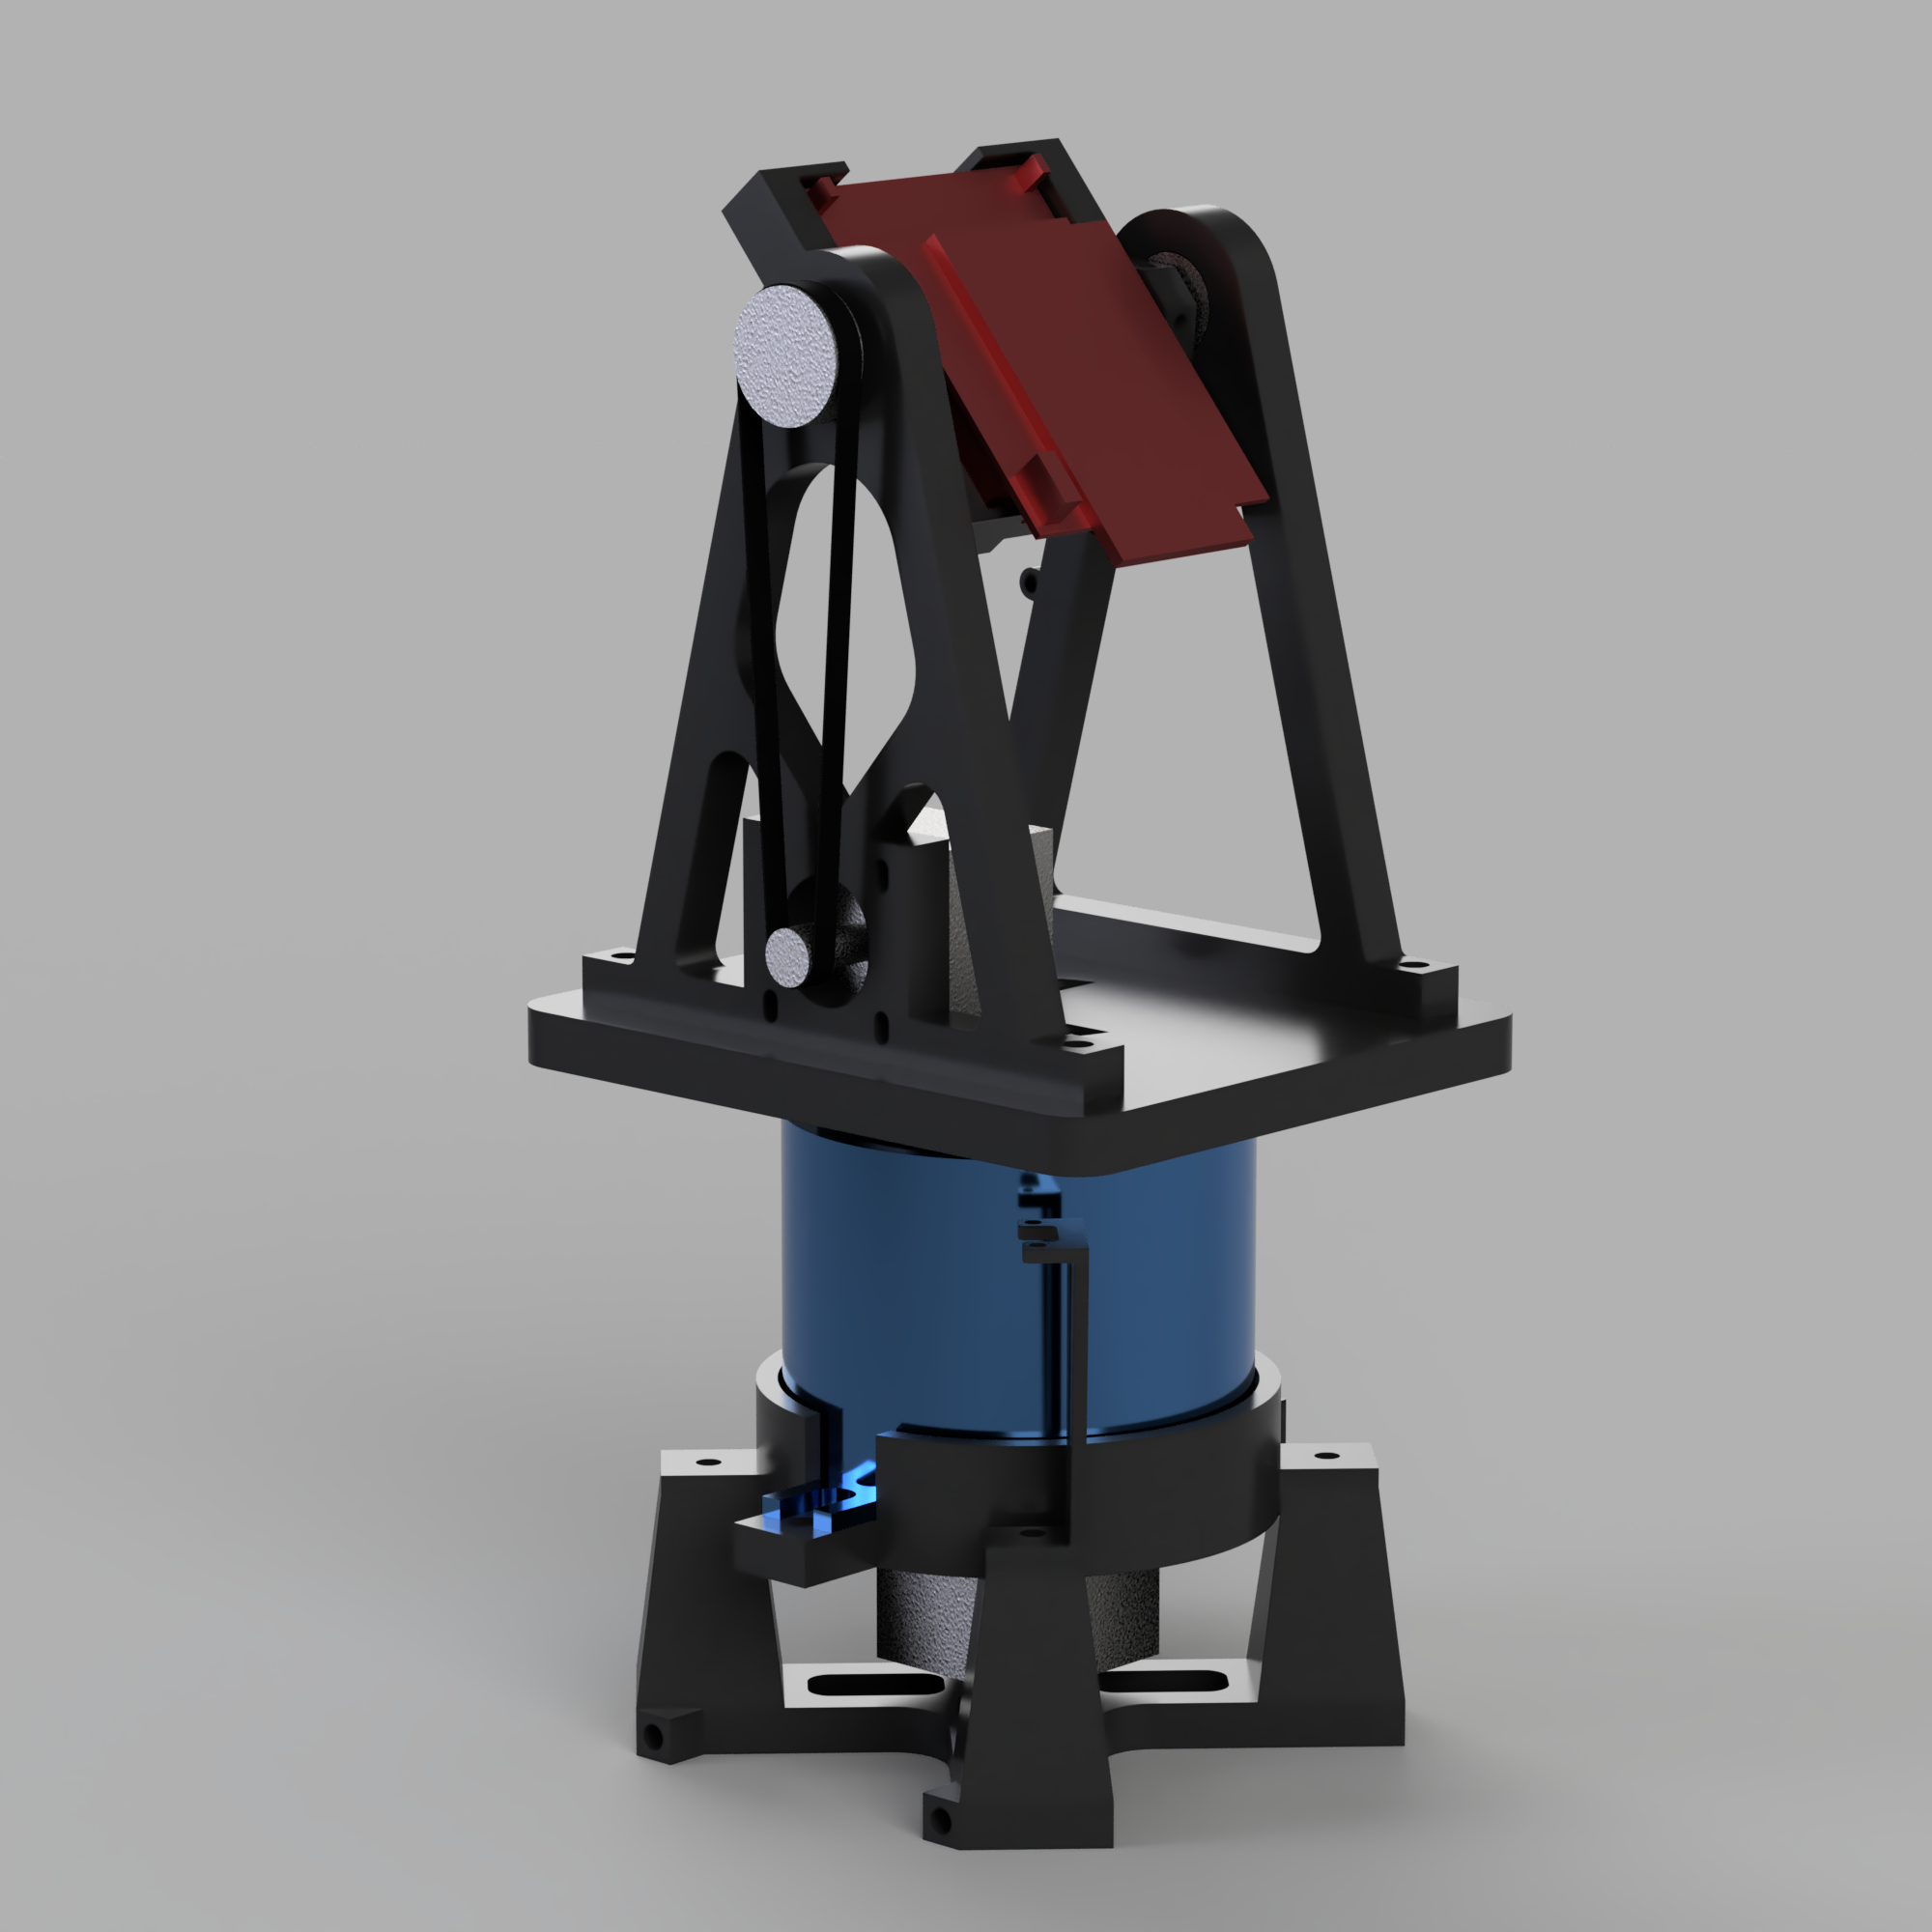
\includegraphics[width=0.85\textwidth]{../img/whole_assembly_2.png}
    \caption{3D render}
  \end{subfigure}
  \hspace{0.05\textwidth} % Adjust spacing
  \begin{subfigure}[b]{0.35\textwidth}
    \centering
    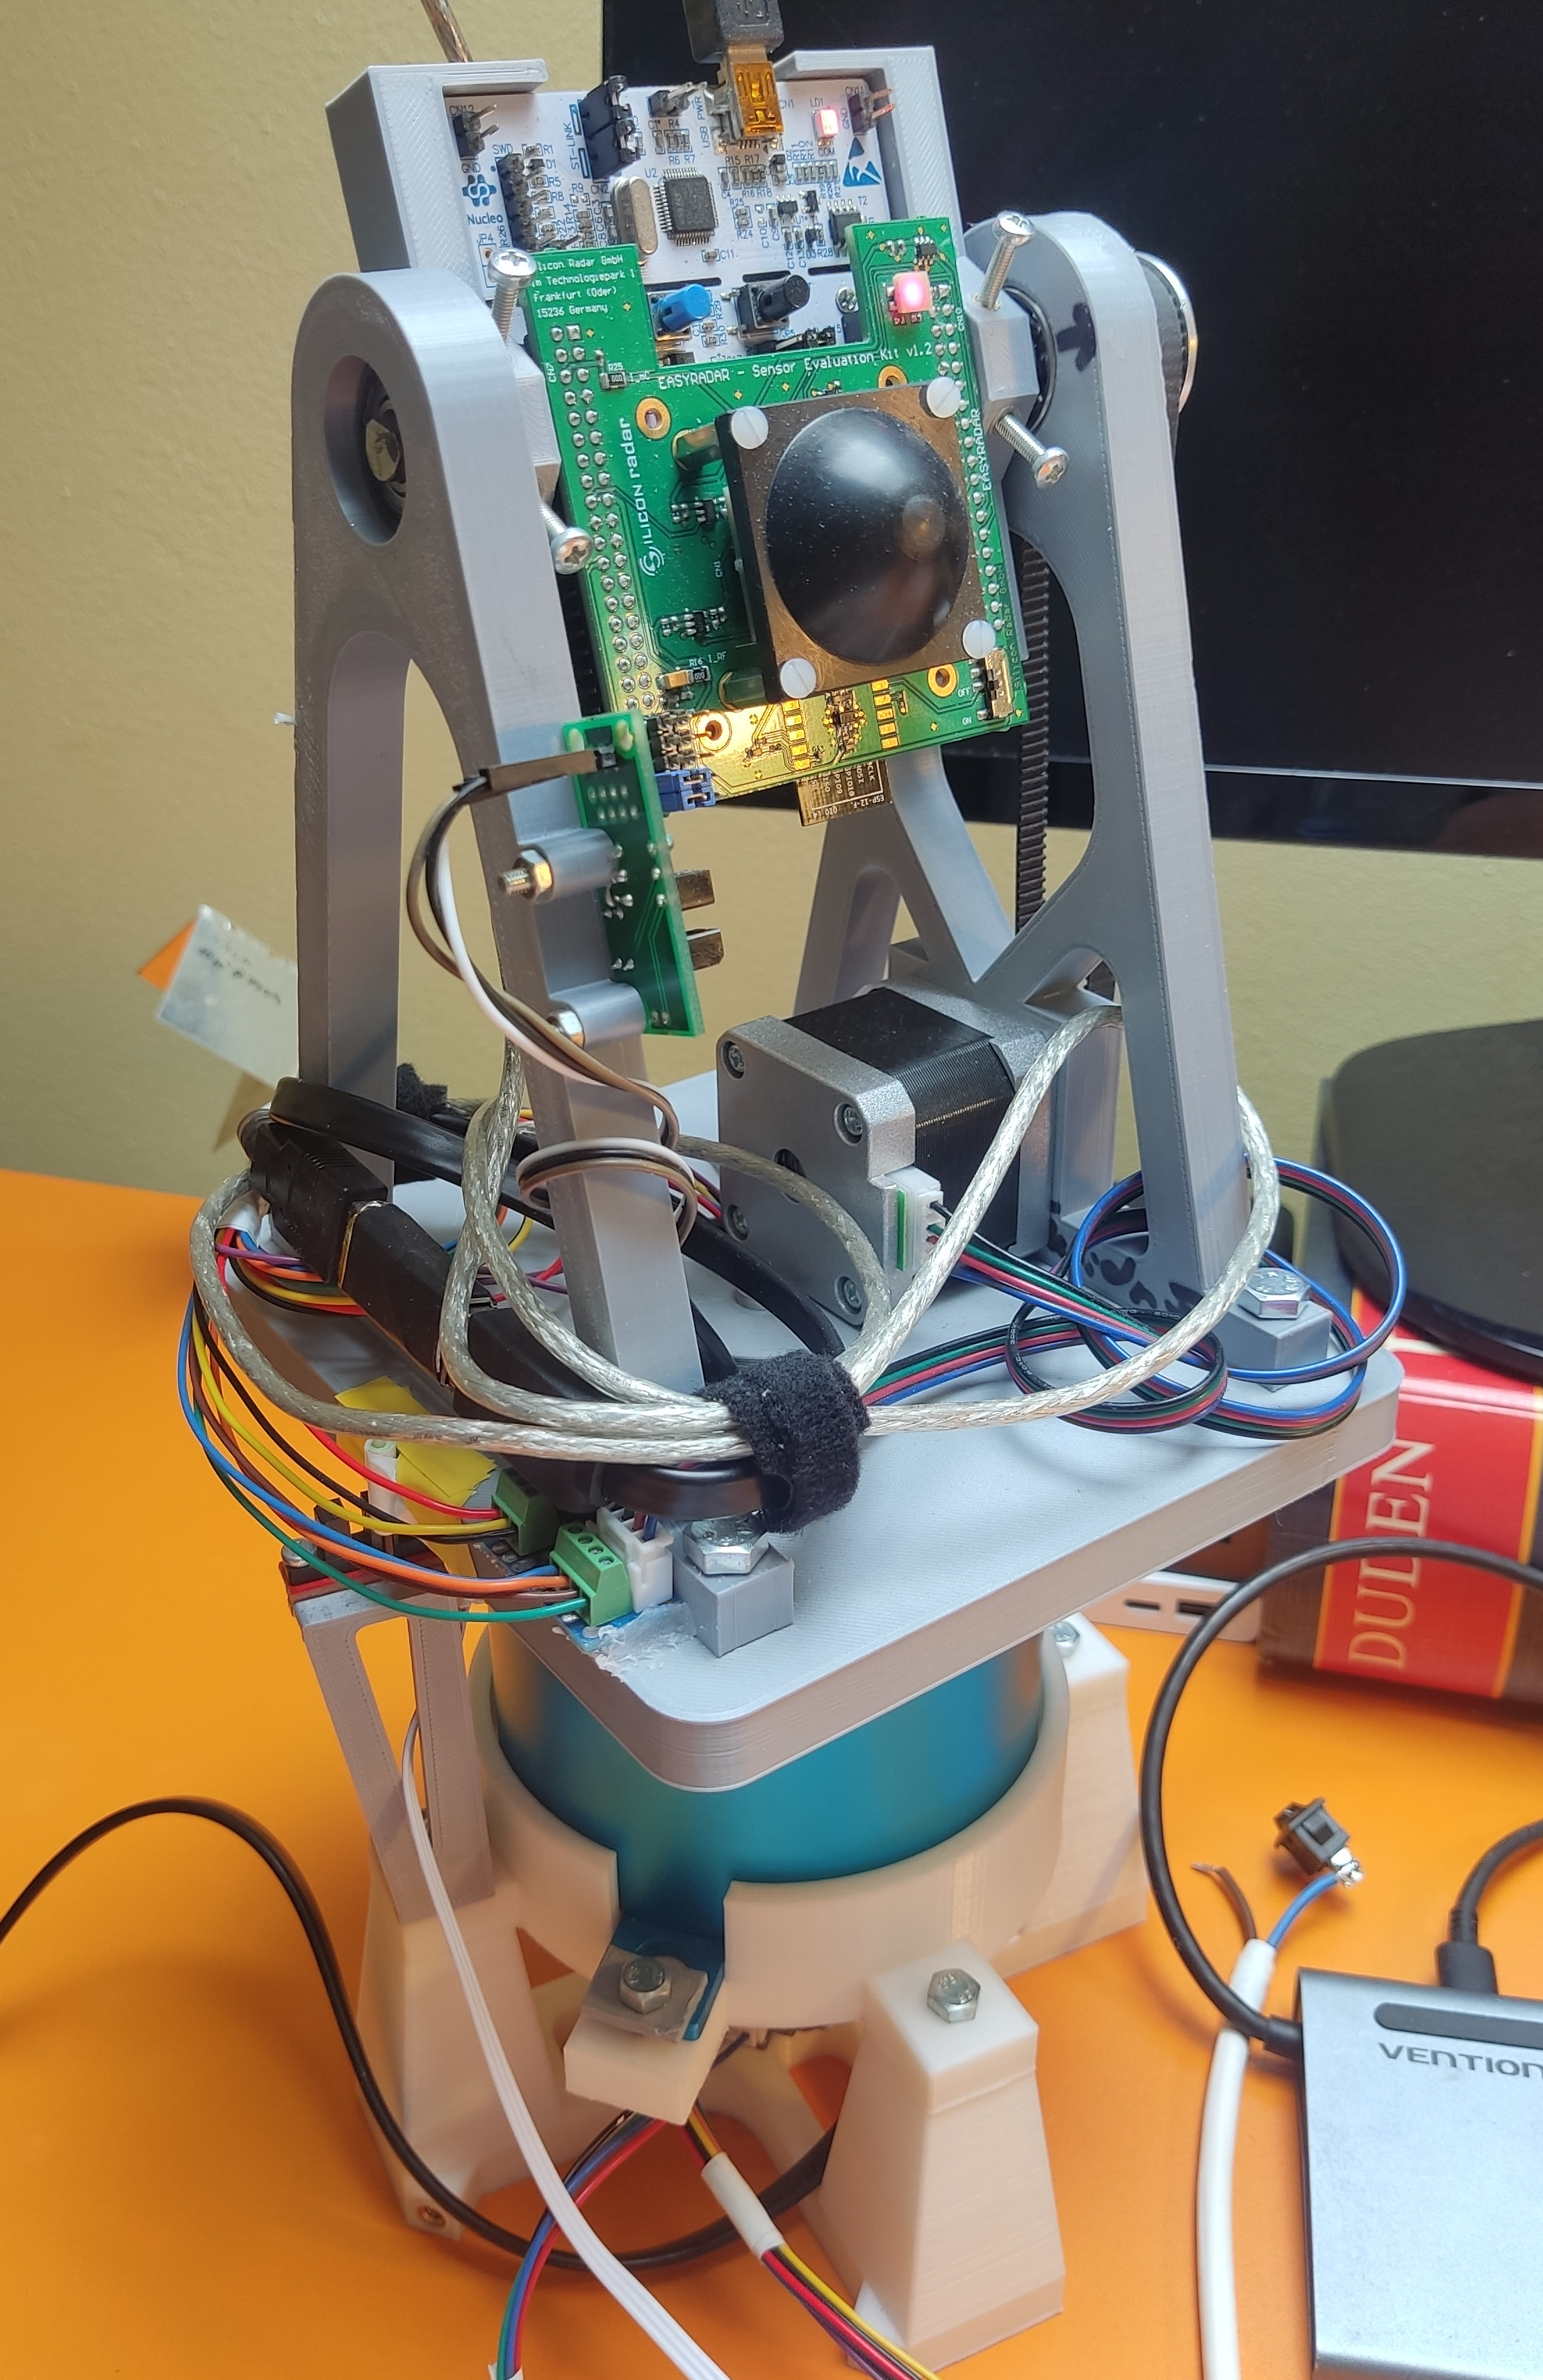
\includegraphics[width=\textwidth]{../img/assembly_photo.jpg}
    \caption{Photo}
  \end{subfigure}
  \caption{Form of the final assembly}
  \label{fig:side_by_side}
\end{figure}


\subsection{Platform Electronics}

The electronic side of the platform is relatively simple.
Only two problems needed to be tackled: driving the stepper motors and implementing a homing mechanism.

Given the platform cannot generate any significant momentum that could potentially lead to skipping steps a basic stepper driver without feedback control was deemed sufficient.
In the project A4988 stepper driver was chosen due to its low cost, up to 1:16 microstepping capabilities, and basic current control.
A minor drawback of it is the lack of any feedback from the driver to the microcontroller, including stall detection \cite{a4988}.

Since the number of components is quite low and there aren't any special requirements for the circuit, just a simple prototyping board  (Figure~\ref{fig:circuit}) was used instead of designing a custom PCB.
This decision also makes it easier to replace the driver in case of failure.
Or even enables an upgrade path via more modern chips, such as the TMC2208 or TMC2209 as their devkits are pin-compatible with the A4988 \cite{a4988_sound}.
This might be necessary in use cases where the platform's volume level would be a serious problem.
The A4988 produces a rather noisy driving signal and more modern drivers exhibit up to 20~dB lower noise levels \cite{a4988_sound}.

For homing implementation, two potential solutions were considered: Hall effect sensors and optical gates.
Hall effect sensors offer the advantage of angle sensing, allowing correction for positional drift during operation; however, they require precise alignment.
If the Hall effect sensor is not perfectly placed along the axis of rotation, calibration becomes necessary \cite{hall}.
While feedback would be beneficial, the microcontroller already tracks each step taken by the motor during normal operation, making it possible to determine the platform's position purely in software.
Thus, for simplicity and ease of integration, optical gates were selected.

The system is controlled by an ESP32 microcontroller.
The ESP32-C6 version was chosen due to the author's extensive experience with this particular model.
Still, since the system does not require specialized peripherals or high processing power, most other microcontrollers could have been used instead.

\begin{figure}[h!]
	\centering
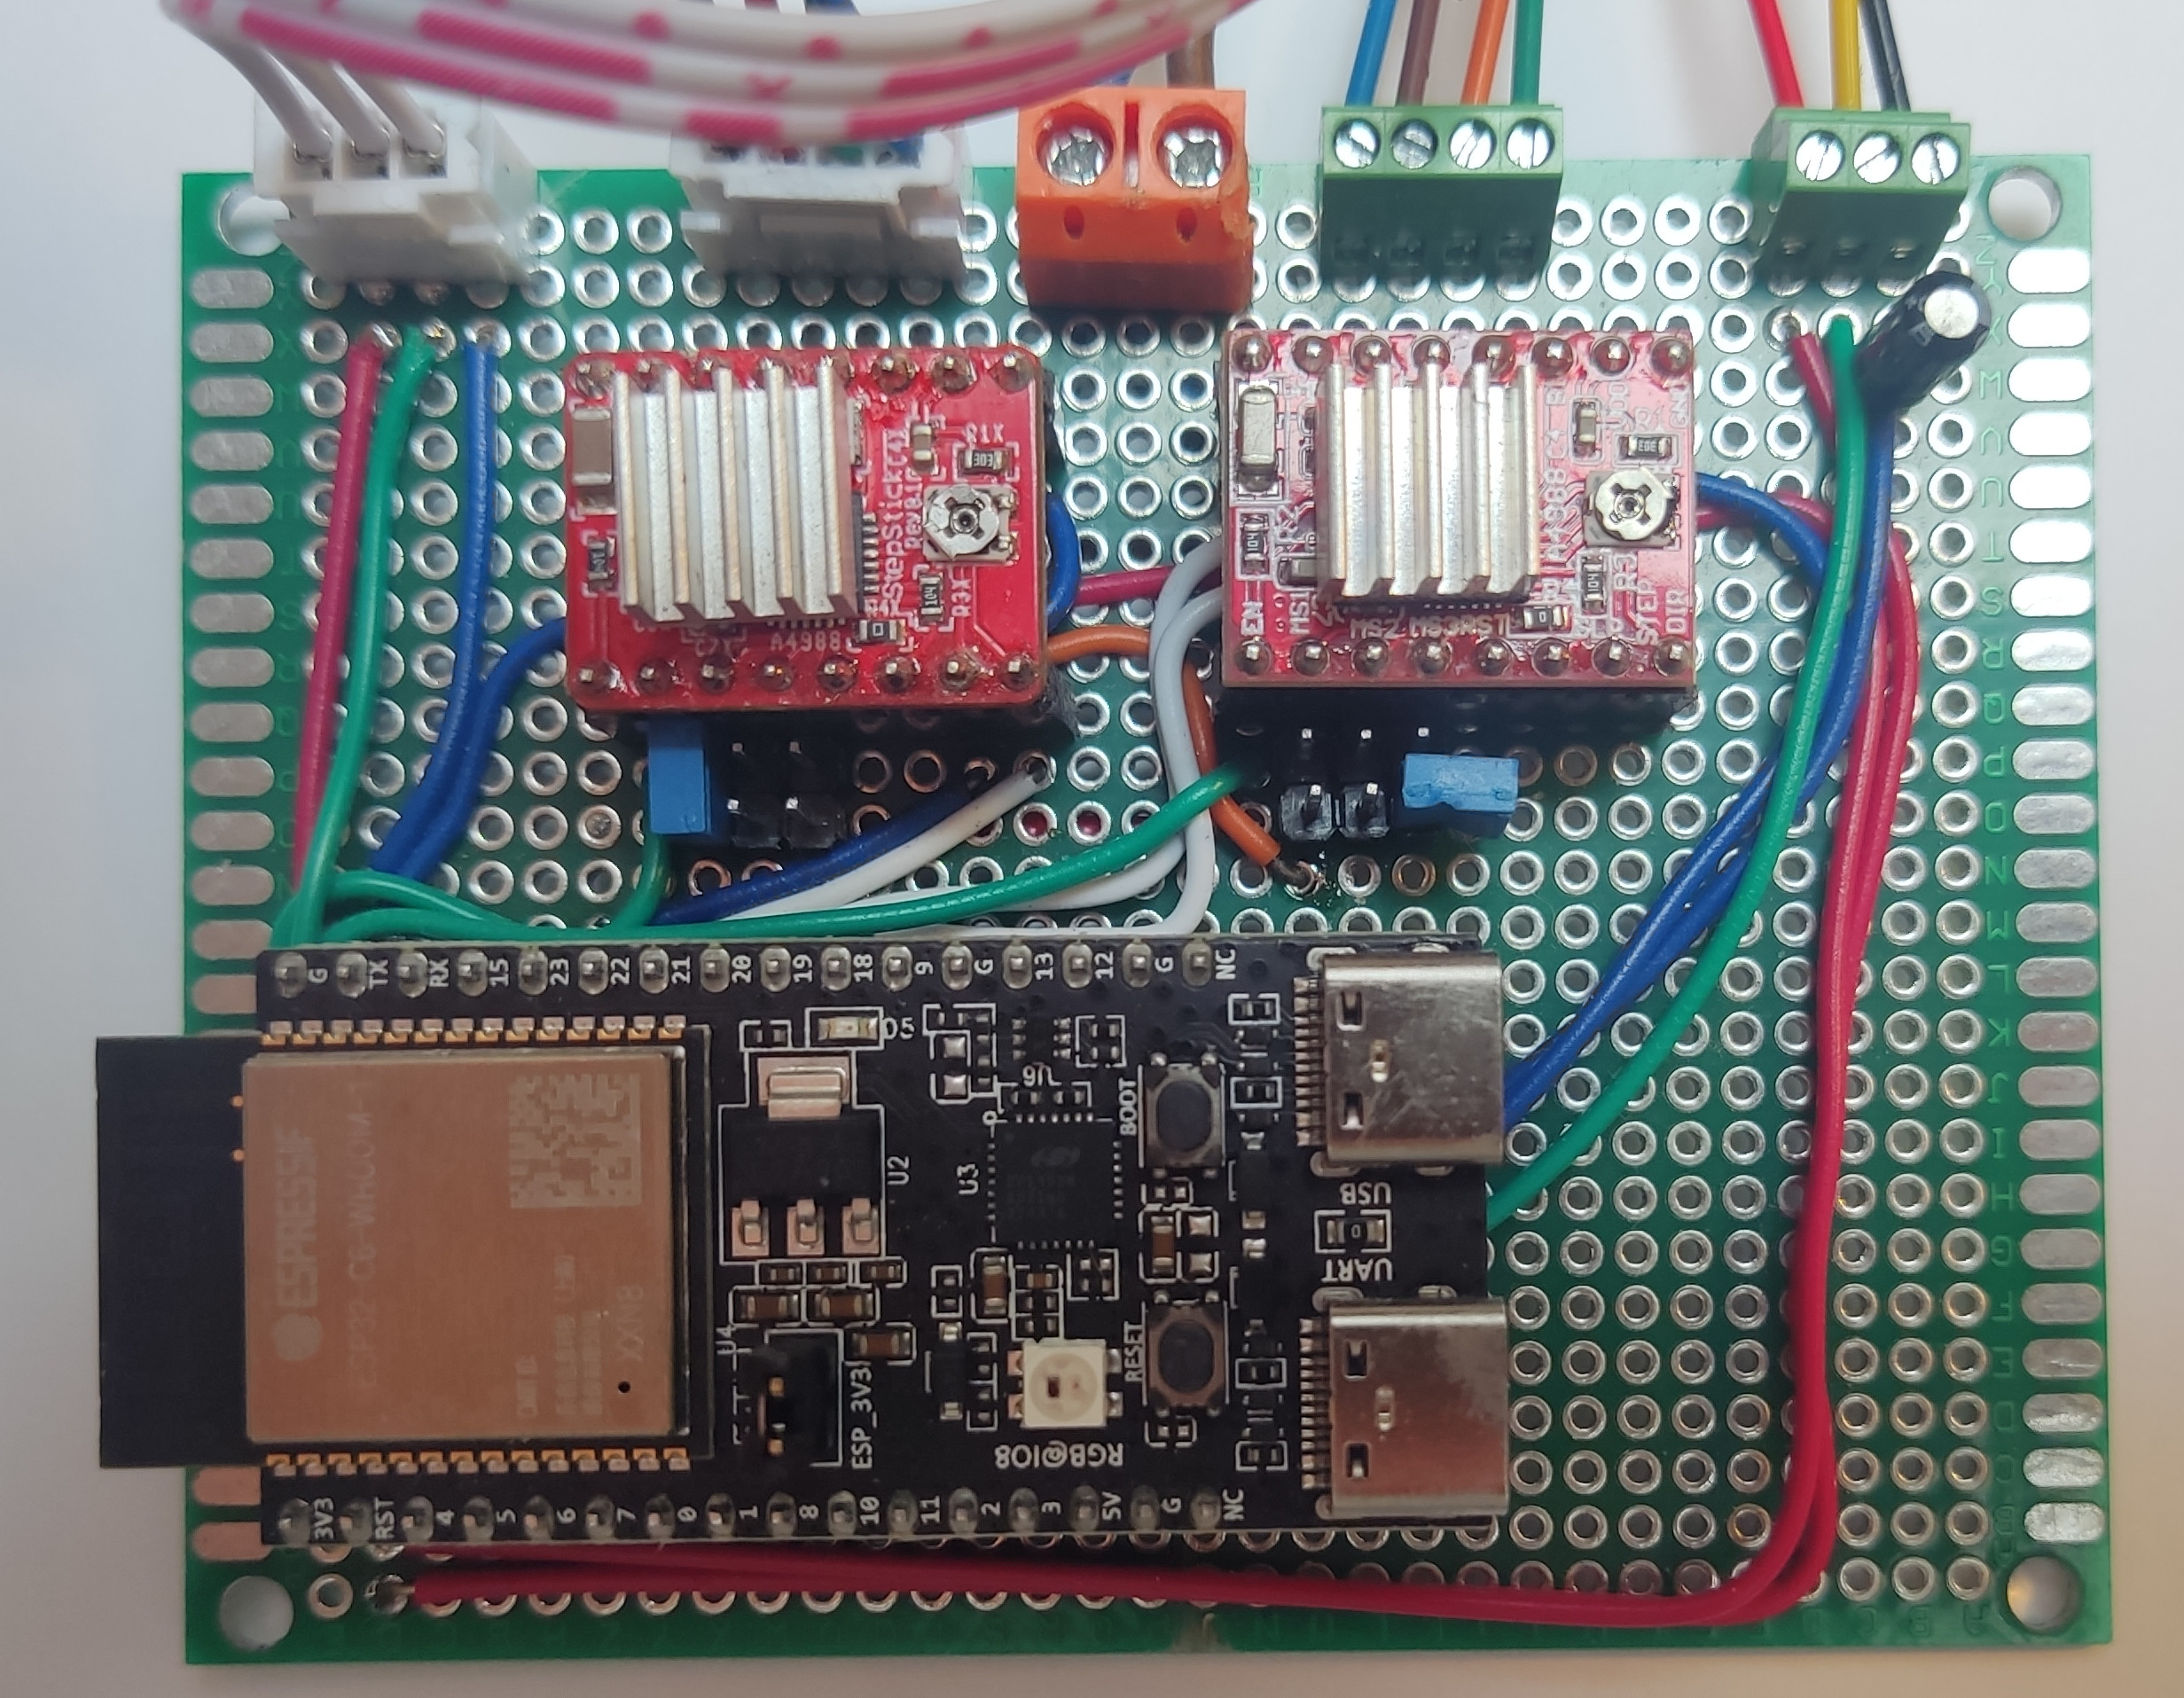
\includegraphics[width=0.7\textwidth]{../img/circuit.jpg}
	\caption[Driving circuit of the platform]{Driving circuit of the platform}
	\label{fig:circuit}
\end{figure}

\section{Platform Software}

Given its widespread adoption as an industry standard for controlling similar machines, G-code over serial is a natural choice for the platform's communication format.
Beyond the basic functionality typically offered by basic G-code interpreters, the platform should support additional features to reduce the user's manual control burden.
These include common features such as defining movement limits, absolute/relative positioning modes, spindle mode and automatic homing.
Lastly, the platform should support a programming interface that allows an application to send an entire choreography of movements to the platform at once, after which it only needs to monitor its status.

For uplink communication, the platform must provide real-time information about its current position.
This data then enables the user to make necessary mathematical corrections and properly interpret the radar's gathered data.

To maximize efficiency in processing commands and ensure accurate stepper motor control, the program workflow is divided into three distinct layers, as illustrated by figure~\ref{fig:code_diag}.
The commonly used two-component architecture—where one component handles communication and command parsing, and the other manages execution—was deemed unsuitable for this use case.
Such an approach would complicate the integration of a programming interface and require just-in-time processing of commands, which could lead to performance issues.

In the chosen architecture, the degree of abstraction decreases with each successive layer, simplifying processing at each step.
This design allows the final layer to operate with maximum efficiency, where the transition from one command to the next is nearly instantaneous.

It is necessary to note that the platform does not store any permanent configuration, including microstepping settings.
This approach was taken because the platform does not offer any easy way to display the current settings and is expected to be operated only from a computer application.
Thus, instead of needing to keep track of which settings are on the PC and which are stored on the platform, a simpler approach was taken.

\begin{figure}[h!]
  \centering


  \begin{tikzpicture}[scale=0.9, node distance=1.5cm]

    % Layer headers
    \node (comm_layer) [layerheader] at (0, 0) {Communication Layer};
    \node (app_layer) [layerheader] at (6, 0) {Application Layer};
    \node (hal_layer) [layerheader] at (12, 0) {HAL Layer};

    % Communication Layer
    \node (comm_start) [startstop, below of=comm_layer, yshift=-0.3cm] {Start};
    \node (wait_serial) [process, below of=comm_start] {Wait for serial data};
    \node (parse_gcode) [process, below of=wait_serial] {Parse G-code};
    \node (parse_success) [decision, below of=parse_gcode, align=center, yshift=-1.3cm] {Parsing\\ Successful?};
    \node (store_command) [process, below of=parse_success, align=center, yshift=-1.8cm] {Store command\\ queue ? program};
    \node (send_response) [process, below of=store_command,yshift=-0.25cm] {Send response};

    % Arrows in Communication Layer
    \draw [arrow] (comm_start) -- (wait_serial);
    \draw [arrow] (wait_serial) -- (parse_gcode);
    \draw [arrow] (parse_gcode) -- (parse_success);
    \draw [arrow] (parse_success.east) -- ++(1, 0) |- (send_response.east) node[midway, left, yshift=+0.25cm] {No};
    \draw [arrow] (parse_success.south) -- ++(0, -0.5) -| (store_command.north) node[midway, right, yshift=+0.05cm] {Yes};
    \draw [arrow] (store_command) -- (send_response);
    \draw [arrow] (send_response.west) -- ++(-0.5, 0) |- (wait_serial.west);

    % Application Layer
    \node (app_start) [startstop, below of=app_layer, yshift=-0.3cm] {Start};
    \node (update_position) [process, below of=app_start] {Update position};
    \node (check_queues) [decision, below of=update_position, yshift=-1.3cm] {Queues full?};
    \node (load) [process, below of=check_queues, align=center, yshift=-1.5cm] {Load command \\ queue ? program};
    \node (process_command) [process, below of=load,yshift=-0.25cm] {Process command};
    \node (store_command) [process, align=center, below of=process_command] {Add command \\ to stepper queue};

    % Arrows in Application Layer
    \draw [arrow] (app_start) -- (update_position);
    \draw [arrow] (update_position) -- (check_queues);
    \draw [arrow] (check_queues.east) -- ++(1, 0) |- (update_position.east) node[midway, left, xshift=0.2cm, yshift=+0.25cm,xshift=0.2cm] {Yes};
    \draw [arrow] (check_queues.south) -- ++(0, -0.5) -| (load.north) node[midway, right, yshift=+0.1cm] {No};
    \draw [arrow] (load.south) -- ++(0, -0.5) -- (process_command.north);
    \draw [arrow] (process_command) -- (store_command);
    \draw [arrow] (store_command.west) -- ++(-0.5, 0) |- (update_position.west);


    \node (hal_start) [startstop, below of=hal_layer, yshift=-0.3cm] {Start};
    \node (wait_queue) [process, below of=hal_start] {Wait on queue};
    \node (execute_command) [process, below of=wait_queue] {Execute command};
    \node (wait_command) [process, below of=execute_command] {Wait on command};
    \node (update_info) [process, align=center, below of=wait_command] {Update last \\command};

    % Arrows in HAL Layer
    \draw [arrow] (hal_start) -- (wait_queue);
    \draw [arrow] (wait_queue) -- (execute_command);
    \draw [arrow] (execute_command) -- (wait_command);
    \draw [arrow] (wait_command) -- (update_info);
    \draw [arrow] (update_info.west) -- ++(-0.5, 0) |- (wait_queue.west);

  \end{tikzpicture}

  \caption[Program flow diagram]{Program flow diagram}
  \label{fig:code_diag}
\end{figure}

\subsection{Communication Layer}

The communication layer processes incoming data over the serial line.
Its efficient handling is facilitated with the aid of RTOS queues.
Upon receiving a command, the string is parsed and either pushed to a queue to be executed later or added to a program declaration, in case the user is currently writing a program.
Some special commands, such as those for emergency shut-off, are executed immediately.
For a complete overview of supported commands consult Appendix~A.

Immediately after parsing, a response is sent to the user confirming whether the command was parsed correctly or not.
However, as the communication layer does not and cannot check the command within the context of all previous commands, it is possible that a command will be parsed correctly but its execution will fail in the application layer.

\subsection{Application layer}

The application layer performs two primary functions: tracking the current device position and preparing commands to be sent to the stepper motors.
Aside from the current position, the program also keeps track of the end position of the last scheduled command.
Thanks to this, the application layer is able to make all necessary calculations to facilitate absolute positioning or enforce movement limits.

A key departure from standard G-code interpreters, such as \cite{duet}, is how the platform handles single-axis move commands.
When a move command targets only one axis, the other axis remains free to read the next command and begin its execution.
If this behavior is undesirable, the user must issue commands for both axes simultaneously.
In relative positioning mode, a zero value results in no motion; in absolute positioning mode, the command must specify the current position to prevent movement.

This behavior is a necessary side effect of the spindle regime, which typically can only be toggled on or off dynamically \cite{duet}.
Another consequence of spindle mode is the requirement for separate positioning modes for each axis.
Continuous rotation prevents calculating a move’s end position, making it impossible to compute absolute positioning commands, thus necessitating relative positioning.
However, it would be rather restrictive to force the user to use relative positioning on the second axis; therefore, the positioning modes are independent.

To support other possible applications, a manual override mode was also implemented.
This enables the user to manually push a move command directly to the stepper queues, totally skipping the application layer.
The primary use case for this mode is to allow tracking of targets or use in other applications that require real-time control over the platform.
However, user must keep in mind that in this regime, no limits are enforced and the platform operates strictly in relative positioning mode.

\subsection{HAL Layer}

The final layer manages stepper motor control and provides the application layer with essential data for position calculations.
In its loop, the program waits for the next command in the stepper queue.
Upon receiving a command, it sets up execution, waits for one or both steppers to complete their movement, and then proceeds to the next command.
Since limit and absolute positioning calculations are handled in the application layer, the whole routine remains highly efficient -- the layer just moves stepper a given number of steps, or let's it rotate in case of spindle mode.

The main challenge was the generation of precise PWM signals (used to control stepper motor drivers) and stopping the signal generation after a specific number of steps.
As generating a PWM signal in software is impractical, dedicated ESP32C6 peripherals needed to be leveraged.
There are two main options for this task: Remote Controlled Transceiver (RMT) and Motor Control Pulse Width Modulation (MCPWM) combined with Pulse Counter (PCNT).
While RMT allows smooth PWM frequency adjustments, it has several drawbacks: for example, generating a specific number of pulses is supported only on newer ESP32 models \cite{gitRMT}, synchronization is restricted to its proprietary API, and there is no straightforward way to track progress during a move \cite{espRMT}.

For these reasons, combination of MCPWM and PCNT was chosen.
MCPWM handles pulse generation, while PCNT counts steps, enabling easy control over movement and providing a robust API for step count tracking \cite{espPCNT}.
The only limitation is the PCNT’s 15-bit counter, which caps the maximum steps per move at $\pm$32,767.


\subsubsection{Performance of the HAL Layer}

Table \ref{tab:performancepwm} illustrates the stability of PWM generation by the MCPWM module at various speeds.
Measurements were conducted using a Saleae Logic Pro 16 logic analyzer, with no microstepping enabled.

The results show that frequency deviation is minimal, though the generated speed is consistently marginally faster than the target and the error increases slightly at higher speeds.
Nevertheless, when measuring the time for 24,000 steps at 120~RPM, the relative error in time duration (or speed) was only $\epsilon = -0.004\%$, demonstrating excellent accuracy.


\begin{table}[h!]
  \centering
  \caption[Stability of PWM generation]{Stability of PWM generation}
  \begin{tabular}{| m{2cm} || m{2.5cm} | m{2.5cm} | m{2.5cm} | m{2.5cm} |}
    \hline
    RPM & $f_{\mathrm{desired}}$ (Hz) & $f_{\mathrm{low}}$ (Hz) & $f_{\mathrm{high}}$ (Hz) & $f_\mathrm{avg}$ (Hz) \\
    \hline
    10  & 33.334                      & 33.334                  & 33.334                   & 33.334                \\
    30  & 100                         & 100                     & 100.003                  & 100.002               \\
    60  & 200                         & 200                     & 200.01                   & 200.004               \\
    120 & 400                         & 400                     & 400.02                   & 400.007               \\
    \hline
  \end{tabular}
  \label{tab:performancepwm}
\end{table}

\begin{figure}[h!]
  \centering
  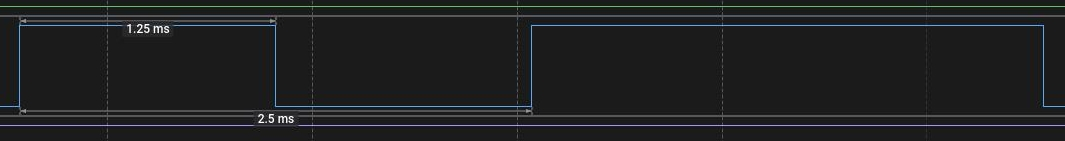
\includegraphics[width=\textwidth]{../img/120rpm_to60_1.jpg}
  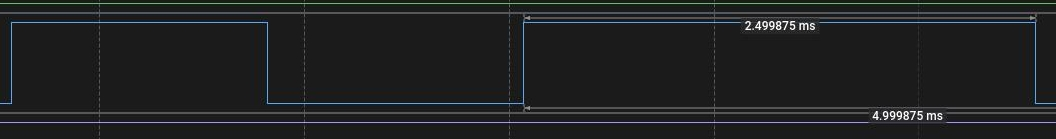
\includegraphics[width=\textwidth]{../img/120rpm_to60_2.jpg}
  \caption[Moment of change between commands with 120RPM and 60RPM]{Moment of change between commands (120RPM $\Rightarrow$  60RPM)}
  \label{fig:switching}
\end{figure}

An attempt was made to also measure the delay between switching commands, as displayed in figure~\ref{fig:switching}.
The results indicate that the delay between commands is imperceptible.
Similar outcomes were also observed for other command combinations.

This demonstrates the efficiency of the HAL layer in managing stepper motor control and transitioning seamlessly between commands.
As long as the stepper queues are supplied with commands in advance, the platform can operate without noticeable interruptions.

\chapter{Control Application}

As previously stated, the control application for the whole system is written in MATLAB.
There are two main parts to it: one is managing the platform and the other for processing radar data.
Alongside these, there are some shared components, such as the preferences menu.

\section{Main Window}

Upon starting the application, the user is presented with the main window (Figure~\ref{fig:main_window}).
This window is primarily used to display radar data and control the basic functionality of the application.
On the sidebar, the user can enable serial connections to the radar and the platform, pause processing, save the current visualization to JPG, and stop the platform in case of an emergency.
Lastly, the top bar allows access preferences and the platform control interface.

\begin{figure}[h!]
  \centering
  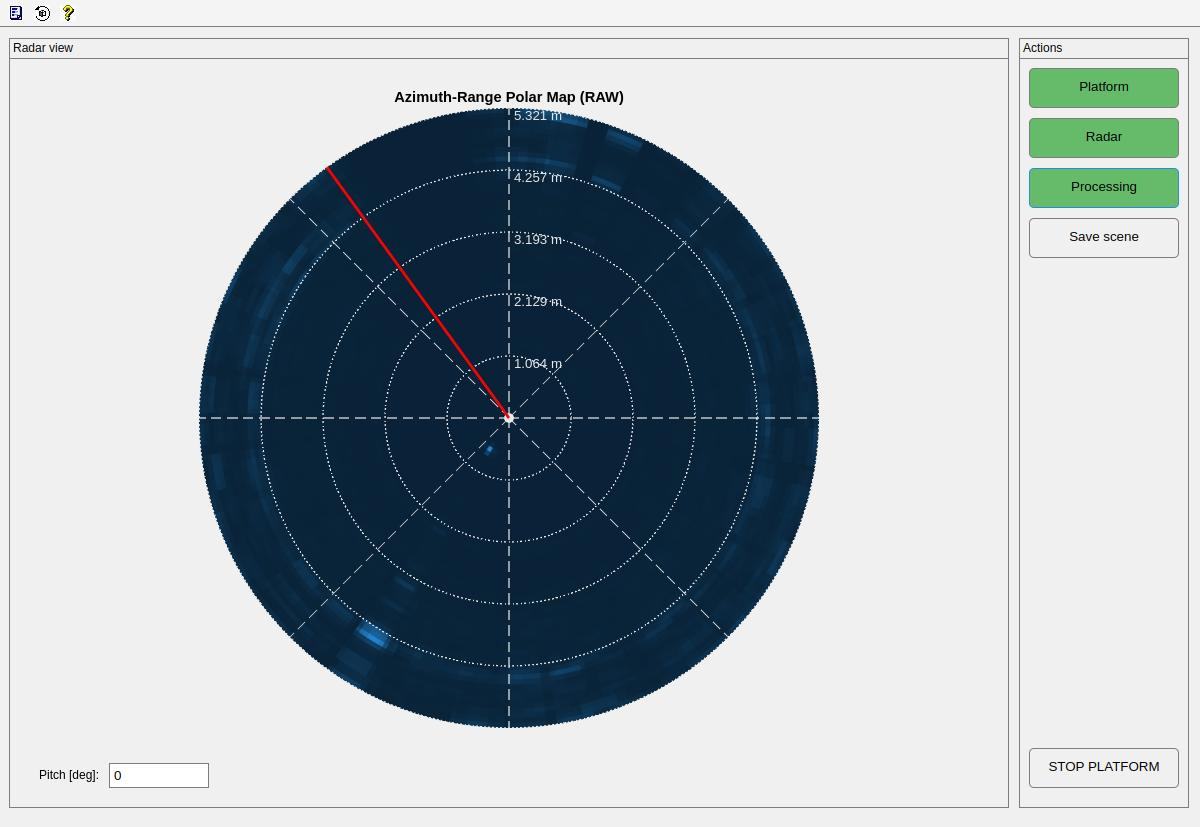
\includegraphics[width=0.9\textwidth]{../img/vis_range_azimuth.jpg}
  \caption[Main application window]{Main application window}
  \label{fig:main_window}
\end{figure}

\subsection{Application Configuration}

As this thesis concerns itself with a rather generic implementation of a surveillance radar system, the application is designed to be as flexible as possible.
For this purpose, a GUI menu was designed to enable configuration of all important elements -- configuring the platform, radar, data processing, and data visualization.
However, it is necessary to point out that, given the extensive configuration options, the user is expected to have some knowledge about the subject to achieve satisfactory results.
Firstly, configuration options are not checked against each other to verify if they are mutually exclusive.
For example, for speed calculation, ramp averaging must be turned off, but as things stand, the application will allow the user to continue even with it enabled.
Secondly, configuration of components such as CFAR or DBSCAN strongly depends on bandwidth, number of samples, FFT point count, and other parameters.
A CFAR guard parameter of 3 might be too small on a 5~GHz bandwidth with a single range bin width of 50~mm, but with $BW=500$~MHz it could be way too large.
To aid in choosing correct parameters, the application provides some basic information, like the dimensions of the bins.
Still, it is up to the user to make the final decision.

Figure~\ref{fig:preferences} shows the preferences menu; as one can see, there are four main sections.
The first configures serial port connections to the radar and the platform.
The second section handles configuration of the platform, followed by a section designated for radar configuration.
The last section configures how the data are processed and via which method they are visualized.

\begin{figure}[h!]
  \centering
  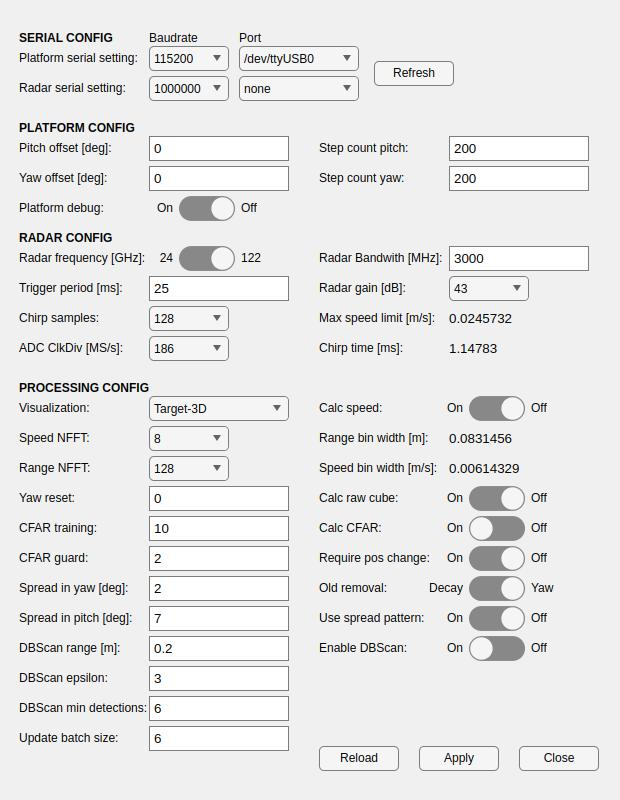
\includegraphics[width=0.7\textwidth]{../img/preferences.jpg}
  \caption[Preferences menu]{Preferences menu}
  \label{fig:preferences}
\end{figure}

User preferences are stored in an INI file in a directory whose path depends on the operating system used—\texttt{\%APPDATA\%/Local/fmcw/fmcw.conf} on Windows and \texttt{\$HOME/.config/fmcw/fmcw.conf} for Unix-based systems.
As INI format is easily human-readable, it is possible to edit the file directly.


\section{Platform Control Interface}

It is necessary to emphasize that the platform control is entirely independent of radar operation.
The user loads a program onto the platform and starts its execution.
From then on, the application only processes current position reports coming from the platform.
There is no feedback from the radar to the platform based on processed data, although, as the platform enables direct access to the stepper queues, it would be possible to implement such a feature.
Nor does processing take into account which movements comprise the platform's current program.

In the preferences menu, the user can configure static offsets to the platform with the \texttt{Pitch offset} and \texttt{Yaw offset} options.
This is useful in case the zero position of the platform is not aligned with what the user wants to be zero in the data.
Aside from offset, step count configuration is also available here with \texttt{Step count pitch} and \texttt{Step count yaw}.
Step count takes into account both microstepping and the physical down-gearing ratio.
It is important to note that, as the platform doesn't store the step count in non-volatile memory, this setting is essential to maintain proper operation of the platform.
The step count command is sent to the platform each time it is connected or the configuration is changed.
Lastly, the \texttt{Platform debug} toggle enables full debug output to be visible in the platform control window.

\begin{figure}[h!]
  \centering
  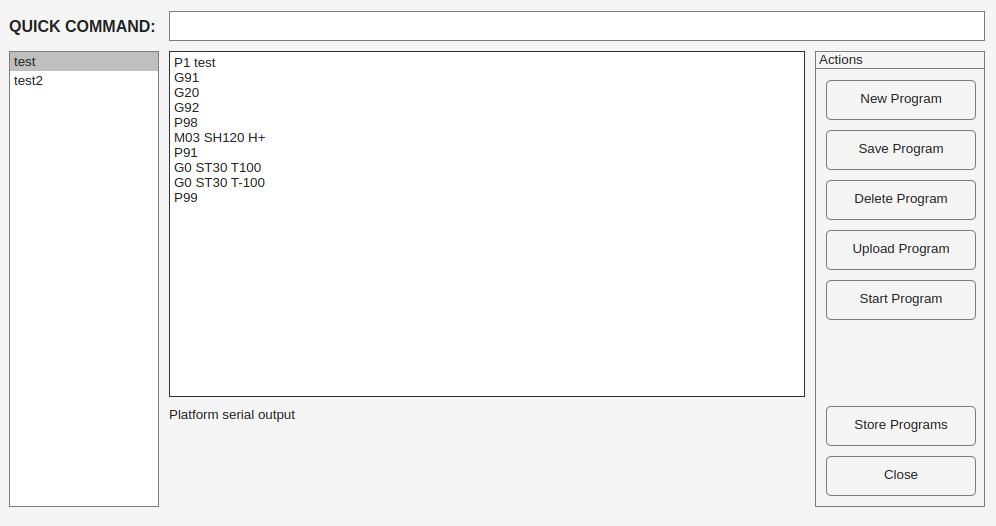
\includegraphics[width=\textwidth]{../img/platform_control.jpg}
  \caption[GUI of the platform control]{GUI of the platform control}
  \label{fig:platformControl}
\end{figure}

Managing platform programs is done via a separate window (Figure~\ref{fig:platformControl}).
This interface enables the user to load, edit, and send programs to the platform.
The left sidebar allows the user to load stored programs by clicking on their name.
The middle text boxes are used to edit the program header (top part) and program body (middle part), with the bottom text field being used to display the platform's debug output.
On the right side are buttons that handle basic operations on the program: load, save, store to file, upload, and start.

Commands are written one per line; their complete syntax is described in Appendix~A.
Control commands used to denote the start of a program, end of header, and so on are automatically sent to the device when the rest of the program is uploaded.
To validate whether the program was parsed correctly, the user can check the text window at the bottom of the screen, which forwards the platform's debug output.
If the user clicks the store button, the program is stored in the same INI file as the preferences.


Backend side of the platform control is rather straightforward.
After a connection is established, the MATLAB serial interface calls a callback each time a terminator sequence is found in received data.
The received message is then parsed, with debug output being forwarded to the user and positions logged with a timestamp in a circular buffer.
The radar data processing part can then request a list of positions for a given time interval.

Platform control can also emit an event when the platform finds itself close to a predetermined position.
This angle is specified in the \texttt{Reset yaw} option, with a tolerance zone fixed at two degrees on either side.
In order to prevent multiple triggering of the event, the program will only emit it once per 1~s.
When the \texttt{Cube decay} option is set to 'reset', if this event is used to clear stored data after a cycle is completed,

\section{Radar configuration}

Given that the radar's output is displayed in the main window, there isn't any specialized interface dedicated just to the radar.
Still, in the preferences menu, there are some parameters that can be configured.

The \texttt{Radar frequency} toggle chooses between the 24~GHz and 122~GHz headers.
However, this only affects the configuration sent to the radar; it does not reflash the firmware, which is also necessary.
After the base frequency, \texttt{Radar bandwidth} can also be configured; both positive and negative values are accepted, however manual verification is required to ensure that the radar is working as expected.
While the manufacturer states a 3~GHz limit on the 24~GHz header and 5~GHz on the 122~GHz header \cite{siradPRO}, in practice—especially with the 24~GHz header—achievable bandwidth was usually much lower and its limit was rather inconsistent.

The user can also configure the number of samples per chirp via \texttt{Chirp samples} and the ADC rate with \texttt{ADC ClkDiv}.
These two parameters determine the time of a single ramp, which is calculated with equation~(\ref{eq:sampling}).
Together with gain, ramp time plays a crucial role in maintaining a good signal-to-noise ratio.

The drop-down menu \texttt{Ramp coherent avg} allows the user to pick how many ramps will be averaged together.
However, use of this feature is generally not recommended unless the surrounding environment is too cluttered.
Each ramp adds about 2~ms overhead to the radar's operation and makes speed calculation impossible.

The last parameter is \texttt{Trigger period}, which dictates how often the application will send a trigger command to the radar.
As previously stated, the radar is at best capable of a chirp roughly every 20~ms.

\chapter{Radar Data Processing}

Firstly, it is necessary to outline the inputs and outputs of the entire processing pipeline.
Data are arrive to the application from two sources: serial connections to the radar and to the platform.
These two data streams are then paired together based on timestamps logged when the data are received.
Program then performs user-selected calculations -- components such as CFAR calculation, speed calculation, and so on can be enabled or disabled as needed.
After processing finishes, the output data are stored in a radar cube, a common method for managing radar data that enables easy integration of more complex algorithms in the future \cite{richards2022}.

Given that both CFAR and raw data (that is, individual range-Doppler maps) calculations might be enabled at the same time, the application maintains two radar cubes.
One is a 4D structure with dimensions of fast time $\times$ slow time $\times$ yaw $\times$ pitch, used to store the complete range-Doppler map for each spatial degree.
In this thesis, this structure is only used for visualizing raw data for a given fixed pitch angle or for showing the range-Doppler map for a given yaw and pitch.
Any 3D visualization style of the raw data would be too cluttered and hard to interpret.
The second cube is a 3D structure with dimensions of range $\times$ yaw $\times$ pitch; this one is used to store CFAR output.

In each case, the yaw resolution is fixed at 1 degree, thus the cube is 360° wide.
Given the quality of the radar mounting bracket, the 1.8° resolution of the stepper, and the tightness of the radiation pattern, a 1° resolution was deemed sufficient.
As for pitch, the same resolution was kept, with angles ranging from -20° to +80° being covered.
The lower bound is limited by the radar's mounting bracket, and the upper bound is more or less arbitrary, slightly motivated by trying to prevent the radar from seeing behind itself.

The main complicating factor in the processing was the need to keep the main thread responsive.
The most time-critical responsibility of the main thread is the timely readout of data from the serial ports.
If data cannot be read immediately upon arrival, the assigned timestamps will be incorrect and, therefore, the data will be attributed to a wrong position.
In addition, the GUI becomes quite unresponsive if the main thread's resources are stretched too thin.

To solve this problem, processing heavily leverages MATLAB's Parallel Computing Toolbox, offloading as much as possible to different cores.
Throughout the entire processing pipeline, there are mechanisms for buffering data into larger batches, and if needed, discarding some in case the software is unable to keep up.
Unfortunately, as MATLAB's parallelization capabilities with threads are rather limited -- external language interfaces do not work, nor do certain file or memory mapping functions \cite{matlabParallel} -- the parallelization needed to be done with processes.
This restricts the application to machines with at least 16~GB of RAM, as each process (of which there are three) requires around 2~GB of RAM.

The processing pipeline can be divided into several distinct steps as follows:
\setlist[enumerate]{nosep, topsep=3pt, partopsep=3pt}
\begin{enumerate}
  \item Data acquisition: Data are read, a simple FFT is calculated, and spectra are buffered into a circular buffer.
  \item Data processing: Spectra are retrieved from the circular buffer, paired with positions, and processed.
  \item Cube update: Processed data are buffered into a ping-pong buffer. If the buffer is full, the cube update routine is launched.
  \item Visualization: After cubes are updated, data are visualized.
\end{enumerate}

\section{Data Acquisition}

The basic workflow of this step is shown in figure~\ref{fig:radar_flow}.
The process starts as soon as MATLAB detects a line terminator within the incoming radar data stream.
After the entire frame from the radar is read, the data are timestamped and the I and Q channels are buffered.
The observer \texttt{dataProcessor.m} is then notified and left to retrieve the data when the main thread is free.

After retrieval, the in-phase and quadrature channels are merged to form a complex signal, which is multiplied by a Hann window to prevent spectral leakage.
A basic 1D FFT is then calculated, with the number of points set by the \texttt{Range NFFT} parameter in the preferences.
If the FFT order is larger than the number of samples, zero padding is added.
The resulting spectrum is again buffered in its complex form.
Following this step, the program has in memory multiple FFT spectra -- these can be leveraged to enable range-Doppler map computation.

After the spectrum is stored, the program verifies if the platform has moved.
This check helps save processing resources by avoiding computation of an R-D map that would be immediately overwritten.
After movement is detected, the code then takes all spectra (Except the last one when the platform has changed position.) and launches another processing step in a separate thread.
If the user wishes processing to always take place (e.g., when verifying radar settings while the platform is static), this check can be skipped by toggling \texttt{Require pos change}.

\begin{figure}[h!]
  \centering
  \begin{tikzpicture}[node distance=1.5cm, scale=0.6]

    % Layer headers
    \node (radar_header) [layerheader] at (0, 0) {radar.m};
    \node (processor_header) [layerheader] at (7.5, 0) {dataProcessor.m};

    % Radar Module
    \node (radar_start) [startstop, below of=radar_header, yshift=-0.3cm] {Start};
    \node (read_serial) [process, below of=radar_start] {Read serial data};
    \node (buffer_raw) [process, below of=read_serial] {Buffer raw data};
    \node (notify) [process, below of=buffer_raw] {Notify observers};

    % Data Processor Module
    \node (proc_start) [startstop, below of=processor_header, yshift=-0.3cm] {On notify};
    \node (read_radar) [process, below of=proc_start] {Read radar data};
    \node (calc_fft) [process, below of=read_radar, align=center] {Calculate FFT\\ Buffer spectrum};
    \node (check_pos) [decision, below of=calc_fft, yshift=-1cm, align=center] {Position\\ changed?};
    \node (get_spectrums) [process, right of=read_radar, xshift=4cm, align=center] {Get spectrums};
    \node (get_positions) [process, below of=get_spectrums] {Get positions};
    \node (cfar_process) [process, below of=get_positions, align=center] {Launch 2D/CFAR\\ processing};
    \node (proc_stop) [startstop, below of=check_pos, yshift=-1.3cm] {End};

    % Arrows for Radar Module
    \draw [arrow] (radar_start) -- (read_serial);
    \draw [arrow] (read_serial) -- (buffer_raw);
    \draw [arrow] (buffer_raw) -- (notify);
    \draw [arrow] (notify.west) -- ++(-1,0) |- (read_serial.west);
    %
    % % Arrows for Data Processor Module
    \draw [arrow] (proc_start) -- (read_radar);
    \draw [arrow] (read_radar) -- (calc_fft);
    \draw [arrow] (calc_fft) -- (check_pos);
    %
    % % Yes branch
    \draw [arrow] (check_pos.east) -- ++(1,0) node[right] {Yes} |- (get_spectrums.west);
    \draw [arrow] (get_spectrums) -- (get_positions);
    \draw [arrow] (get_positions) -- (cfar_process);
    %
    % % No branch
    \draw [arrow] (check_pos.south) -- node[right] {No} (proc_stop.north);

    % \draw [arrow] (cfar_process.south) -- ++(0,-1.7) -| (proc_stop.east);
    \draw [arrow] (cfar_process.south) |- (proc_stop.east);
  \end{tikzpicture}
  \caption{Processing flow - Data acquisition}
  \label{fig:radar_flow}
\end{figure}

\section{Data Processing}

A parallel process takes calculated FFT spectra and their accompanying positions and processes them into a single range-Doppler map and an array with CFAR output.
A basic outline of this step is shown in figure~\ref{fig:feature_flow}.

\begin{figure}[h!]
  \centering
  \begin{tikzpicture}[node distance=1cm, scale=0.5]
    % Main horizontal flow
    \node (processor_header) [layerheader] at (0, 0) {dataProcessor.m};
    \node (start) [startstop, below =of processor_header] {Thread start};
    \node (rcs) [process, right = of start] {Calculate RCS};
    \node (cfar_decision) [decision, below = of start] {CFAR?};
    \node (raw_decision) [decision, right=1cm of cfar_decision] {RAW?};
    \node (speed_decision) [decision, right=1.5cm of raw_decision] {Speed?};
    \node (return) [startstop, below=2.6cm of speed_decision] {Return};

    % CFAR branch
    \node (cfar_proc) [process, below=of cfar_decision, align=center] {Calc\\CFAR};


    % Speed branch
    \node (mock) [process, below left=1.5cm and -0.4cm of speed_decision, align=center] {Use last chirp\\ RCS array};
    \node (fft) [process, below right=1.5cm and -0.4cm of speed_decision, align=center] {2DFFT/\\NUFFT};

    % Connections
    \draw [arrow] (start.east) -- (rcs.west);
    \draw [arrow] (rcs.south) -- ++(0,-1) -| (cfar_decision.north);
    \draw [arrow] (cfar_decision.east) -- node[above] {No} (raw_decision.west);
    \draw [arrow] (cfar_decision.south) -- node[right] {Yes} (cfar_proc.north);
    \draw [arrow] (cfar_proc.east)  -- ++(0.3,0) |- (raw_decision.west);
    \draw [arrow] (raw_decision.south) -- ++(0,0) node[left] {No} |- (return.west);
    \draw [arrow] (raw_decision.east) -- node[above] {Yes} (speed_decision.west);
    \draw [arrow] (speed_decision.south) -- ++(0, -0.5) node[above, xshift=-1cm] {No} -| (mock.north);
    \draw [arrow] (speed_decision.east) -- ++(0, 0) node[above, xshift=+0.5cm] {Yes} -| (fft.north);
    \draw [arrow] (mock.south) -- ++(0,0) |- (return.west);
    \draw [arrow] (fft.south) -- ++(0,0) |- (return.east);

  \end{tikzpicture}
  \caption{Processing flow - Data processing}
  \label{fig:feature_flow}
\end{figure}

In the first step, the last spectrum is converted to values proportional to the radar cross section (RCS) of the target.
Starting with equation~(\ref{eq:radar_eq}), we can see that the target's RCS is proportional to the received power divided by the fourth power of the distance to the target.
Range can be calculated from the manufacturer-supplied equation~(\ref{eq:rangeBin}), and power is proportional to the square of values reported from the radar.
Given that the constants of the radar equation change based on configuration, calibration would be required in order to obtain real RCS values.
However, this calibration is not supported, and thus onward, when referring to RCS we refer to values proportional to the RCS, not the actual RCS of the object.

After RCS conversion, if \texttt{Calc CFAR} is enabled, the CFAR algorithm will be executed on the latest chirp in the batch.
In this application, a simple 1D CA-CFAR from MATLAB's Phased Array System Toolbox is used, which is parameterized by two variables: the number of guard bins (those are excluded from the average and are right next to the bin being tested) and the number of training bins (those used to calculate the average) \cite{matlab_cfar}.
Both these parameters are configurable from the preferences menu with \texttt{CFAR training} and \texttt{CFAR guard}.

If raw data calculation is enabled (using the \texttt{Calc raw cube} toggle), the program takes one of two paths depending on whether speed calculation is toggled on or off with \texttt{Calc speed}.
If speed calculation is disabled, the program simply returns half of the original spectrum converted to RCS.

When speed calculation is enabled, the program first cuts off samples that are too far away from the position of the latest chirp in the batch.
After that, the timing of chirps is analyzed to determine whether NUFFT needs to be used.
The decision about which transformation to use is based solely on the ratio of the maximal deviation of the chirp intervals to the median of the chirp intervals; if this ratio is over 20\%, NUFFT is used.
For more accurate measurement, a more complex method should be used, but as the radar timing data are not very precise -- not to mention the radar can track only very slow-moving objects -- this method was deemed sufficient.
For similar reasons, no correction for the platform's movement is applied.
The output range-Doppler map is then shifted in order to create a 2D array with \texttt{Range NFFT} $\times$ \texttt{Speed NFFT} elements, with speed ranging from $-\frac{\text{Speed NFFT}}{2}\cdot w $ to  $\left(\frac{\text{Speed NFFT}}{2}-1\right)\cdot w $, where $w$ is the speed bin width calculated with (\ref{eq:Doppler3}).


\section{Cube Update}

The last step of the processing pipeline handles updates of the radar cubes (Figure~\ref{fig:cube_flow}).
Range-Doppler maps and CFAR data are first buffered in a ping-pong buffer -- where one buffer is used to update the cube while the other one is being filled with new data.
Once the buffer is filled, they switch roles and the cube update routine is launched.

As MATLAB processes do not share the same memory space by default, to avoid redundant copies of the cube, MATLAB's memory mapping is used.
Using the \texttt{memmapfile} function, the cube is mapped to a file on a disk which can be shared between two processes \cite{matlab_memory}.
This approach might lead to some performance degradation if the cube is too large and cannot be held in RAM, but testing showed that for cubes of size 512~MB (roughly a cube for a range-Doppler map of 256 $\times$ 16), the program was still able to keep up with the radar.


\begin{figure}[h!]
  \centering
  \begin{tikzpicture}[node distance=1cm, scale=0.5]
    % dataProcessor.m flow
    \node (processor_header) [layerheader] at (0, 0) {dataProcessor.m};
    \node (proc_event) [startstop, below=of processor_header, align=center] {Chirp processed};
    \node (add_buffer) [process, below=of proc_event] {Add to ping-pong buffer};
    \node (buffer_full) [decision, below=of add_buffer] {Buffer full?};
    \node (start_update) [process, below=of buffer_full] {Start cube update};
    \node (end_func) [startstop, below=of start_update] {End function};

    % radarDataCube.m flow
    \node (cube_header) [layerheader] at (9.5, 0) {radarDataCube.m};
    \node (cube_start) [startstop, below = of cube_header] {Update started};
    \node (keep_raw) [decision, below = of cube_start] {Keep RAW?};
    \node (use_spread) [decision, right=of keep_raw, align=center, xshift=+0.7cm] {Use spread\\pattern?};
    \node (direct_update) [process, below=of use_spread, align=center] {Update raw cube\\decay?};
    \node (create_subcube) [process, below=of direct_update] {Create subcube};
		\node (aggregate) [process, below =of create_subcube, align=center] {Aggregate updates};
		\node (aggregate2) [process, below =of aggregate, align=center] {Update raw cube\\decay?};
    \node (keep_cfar) [decision, below=2cm of keep_raw] {Keep CFAR?};
    \node (update_cfar) [process, below=of keep_cfar, align=center] {Update CFAR cube\\ decay?};
    \node (cube_return) [startstop, below= of update_cfar] {Return};

    % Connections
    \draw [arrow] (proc_event) -- (add_buffer);
    \draw [arrow] (add_buffer) -- (buffer_full);
    \draw [arrow] (buffer_full.south) -- node[right] {Yes} (start_update.north);
    \draw [arrow] (start_update.south) -- (end_func.north);
    \draw [arrow] (buffer_full.west) -- ++(-1.5,0) node[left] {No} |- (end_func.west);
    %
    \draw [arrow] (cube_header) -- (cube_start);
    \draw [arrow] (cube_start) -- (keep_raw);
    \draw [arrow] (keep_raw.east) -- node[above] {Yes} (use_spread.west);
    \draw [arrow] (keep_raw.south) -- node[right] {No} (keep_cfar.north);
    \draw [arrow] (use_spread.south) -- node[right] {No} (direct_update.north);
    \draw [arrow] (direct_update.west) -- ++(0,0) -| (keep_cfar.north);
    \draw [arrow] (use_spread.east) -- ++(1,0) node[above] {Yes} |- (create_subcube.east);
    \draw [arrow] (create_subcube) -- (aggregate);
    \draw [arrow] (aggregate) -- (aggregate2);
    \draw [arrow] (aggregate2.west) -| ++(-0.5,12.396 ) -| (keep_cfar.north);
    %
    \draw [arrow] (keep_cfar.west) -- ++(-1,0) node[above] {No} |- (cube_return.west);
    \draw [arrow] (keep_cfar.south) -- node[right] {Yes} (update_cfar.north);
    \draw [arrow] (update_cfar.south) -- (cube_return.north);
    %
  \end{tikzpicture}
  \caption{Processing flow - Cube update}
  \label{fig:cube_flow}
\end{figure}

The update routine for cubes storing CFAR and raw data is quite similar in the case the spread pattern is disabled.
New data are simply added to the cube at their respective positions, replacing the old data.
If the cube is set to decay (The \texttt{Cube decay} option is set to 'decay'.), the entire cube is multiplied by a decay factor derived from the platform’s movement speed.
The slower the platform moves, the slower the data decay.
Using this option leads to an output that more visually resembles traditional analogue radar systems, where the most recent data are brighter than the older ones.
However, the user needs to keep in mind that color changes do not mean a change in RCS at that position.
In addition, this operation is rather computationally expensive and is the primary reason updates to the cube need to be buffered.

Even on smaller cubes of around 256~MB, this operation takes in the worst case about 50~ms to complete on a laptop with an i7-10210U CPU.
If this behaviour would be undesirable, decay can be turned off in the settings in favor of a hard reset of the cube based on a trigger at a specified yaw angle.
The rest of the processing is then fast enough to keep up with the data stream without any buffering.

Enabling the spread pattern leads to degradation of the quality of the data in exchange for better visualization quality -- especially in range-azimuth visualization style.
Instead of adding new data to just one position in the cube, the range-Doppler map is spread over a larger area with the aid of a 2D matrix made up of a 2D Gaussian function.
As the data in series are usually close to each other in terms of position, the update process can be made more efficient.
Instead of directly adding these contributions to the full cube, a much smaller cube is created.
That cube covers only the area that will be updated with the new data and is later added to the full cube in one go.
This enables significant speedup, as the smaller memory size enables better caching.
Still, in the case of a more performant radar system, this method would be unnecessary, not to mention it has very little basis in radar data processing theory.

Due to the limited performance of MATLAB on the author's machine, some parts of the cube update routine were implemented in C++ with the aid of MATLAB's MEX interface.
This enabled the use of the AVX2 x86 instruction set extension to speed up floating point operations.
Chiefly, decaying of the cube exhibited roughly a twofold performance increase thanks to SIMD instructions.


\section{Visualization}

After the cube update finishes, the program returns to the main thread and the data are visualized.
The only way the user can see the data is via visualization.
Text output or access via API is not available.
However, the application offers a number of different visualization styles to suit the user's requirements.

\begin{enumerate}
	\item Range-Azimuth: Polar plot with range on the radius and azimuth on the angle.
	\item Range-Doppler: Classical xy plot with range on the x-axis and Doppler on the y-axis; if speed is not calculated, the y-axis is replaced with the RCS value.
	\item Target-3D: CFAR data are displayed in 3D Cartesian space.
\end{enumerate}

\subsection{Range-Azimuth}

This visualization style is used to display the data in a polar plot for a fixed pitch angle, which is chosen by a text box at tbe bottom of the screen.
A demonstration of a Range-Azimuth map can be seen in figure~\ref{fig:main_window}, which captures testing with the 122~GHz header and a rather large bandwidth of 3~GHz, providing only about 5 meters of range.
In the picture, only raw data are displayed; however, this visualization style is also able to display CFAR data or overlay both.

Instead of calculating a projection into the horizontal plane, the data are displayed in a conical projection.
That is, no additional calculations are made and the cone obtained by fixing the pitch angle is simply stretched to a circle.
To aid with orientation in the plot, simple line markers are added to provide range and angle reference points.

This visualization style might be especially useful when paired with the 24~GHz header.
Due to its rather wide radiation pattern, the radar is able to detect objects in quite a large area.
This can be extended even further if the spread pattern is enabled, where more pitch angles will influence the data.
Thus, for a realization of a classical surveillance radar, this method of visualization might be the most versatile.

\subsection{Range-Doppler}

Picking this visualization style from the preferences menu will display the data in a classical x-y plot for a fixed yaw and pitch angle.
Just as with the Range-Azimuth map, both angles are configurable via text boxes at the bottom of the screen.
In cases when speed calculation is disabled, the y-axis is replaced with the RCS value.

The main purpose of this visualization style is to provide a method for verifying radar data processing and settings.
As the devkit does not report many useful errors and its technical documentation is sometimes incorrect (e.g., in allowed bandwidth values), it is useful to have a way to verify that the radar is working as expected.

\begin{figure}[h!]
  \centering
  \begin{subfigure}[b]{0.45\textwidth}
    \centering
    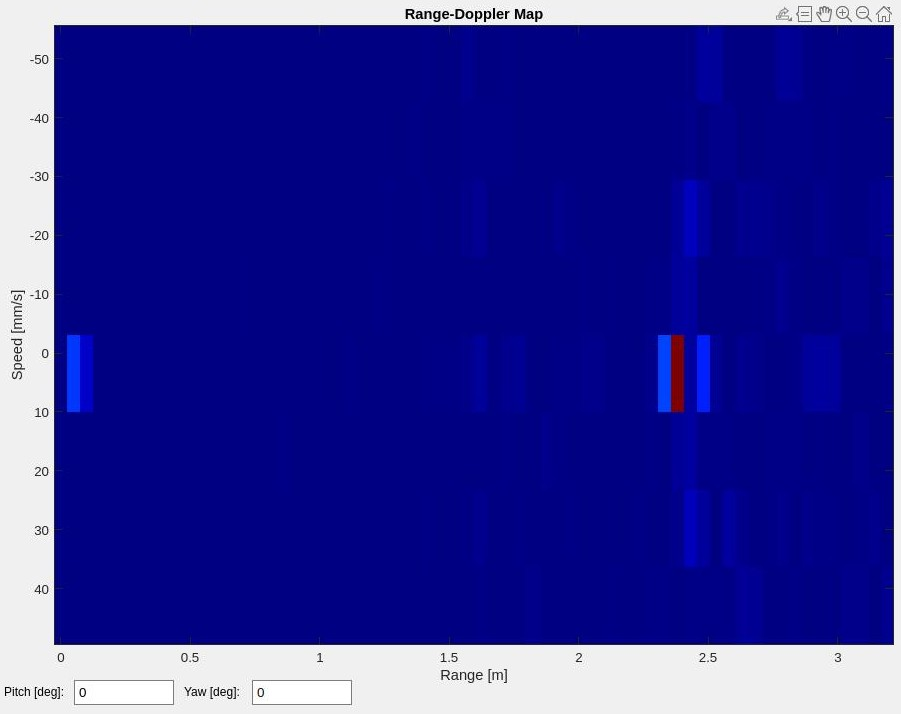
\includegraphics[width=\textwidth]{../img/vis_range_dop.jpg}
    \caption{Range-Doppler map}
  \end{subfigure}
  \hspace{0.05\textwidth}
  \begin{subfigure}[b]{0.45\textwidth}
    \centering
    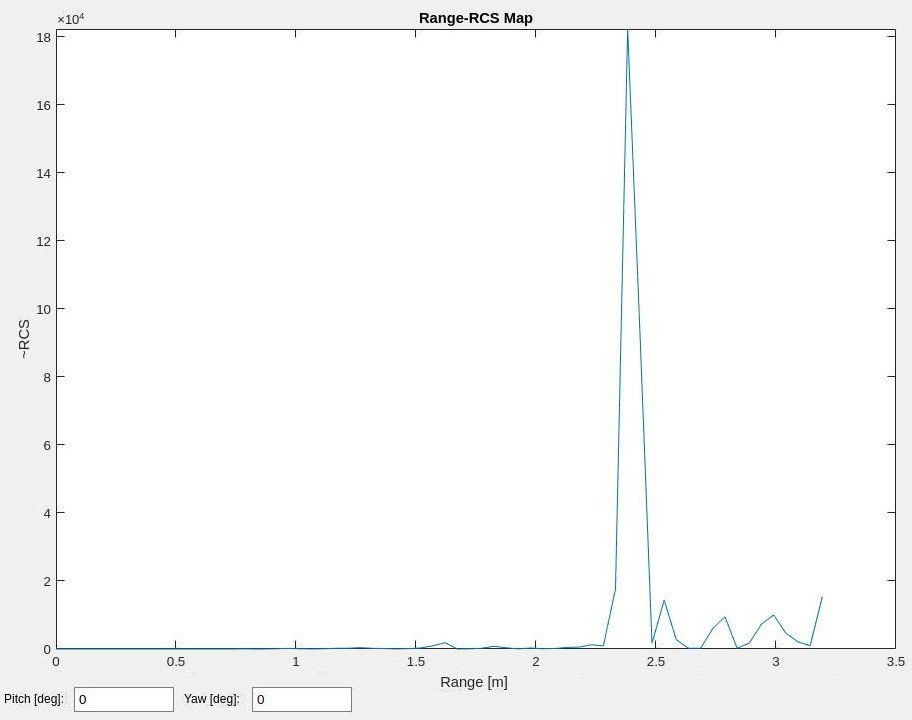
\includegraphics[width=\textwidth]{../img/vis_range_rcs.jpg}
    \caption{Range-RCS }
  \end{subfigure}
	\caption{Range-Doppler and Range-RCS maps}
  \label{fig:rd_rr_map}
\end{figure}

In figure~\ref{fig:rd_rr_map} we can see two different visualization styles, both displaying the same static scene.
As previously stated, given the rather poor sampling rate, speed calculation is not very precise and thus no complex testing has been conducted for it.

\subsection{Target-3D}

\begin{figure}[h!]
	\centering
	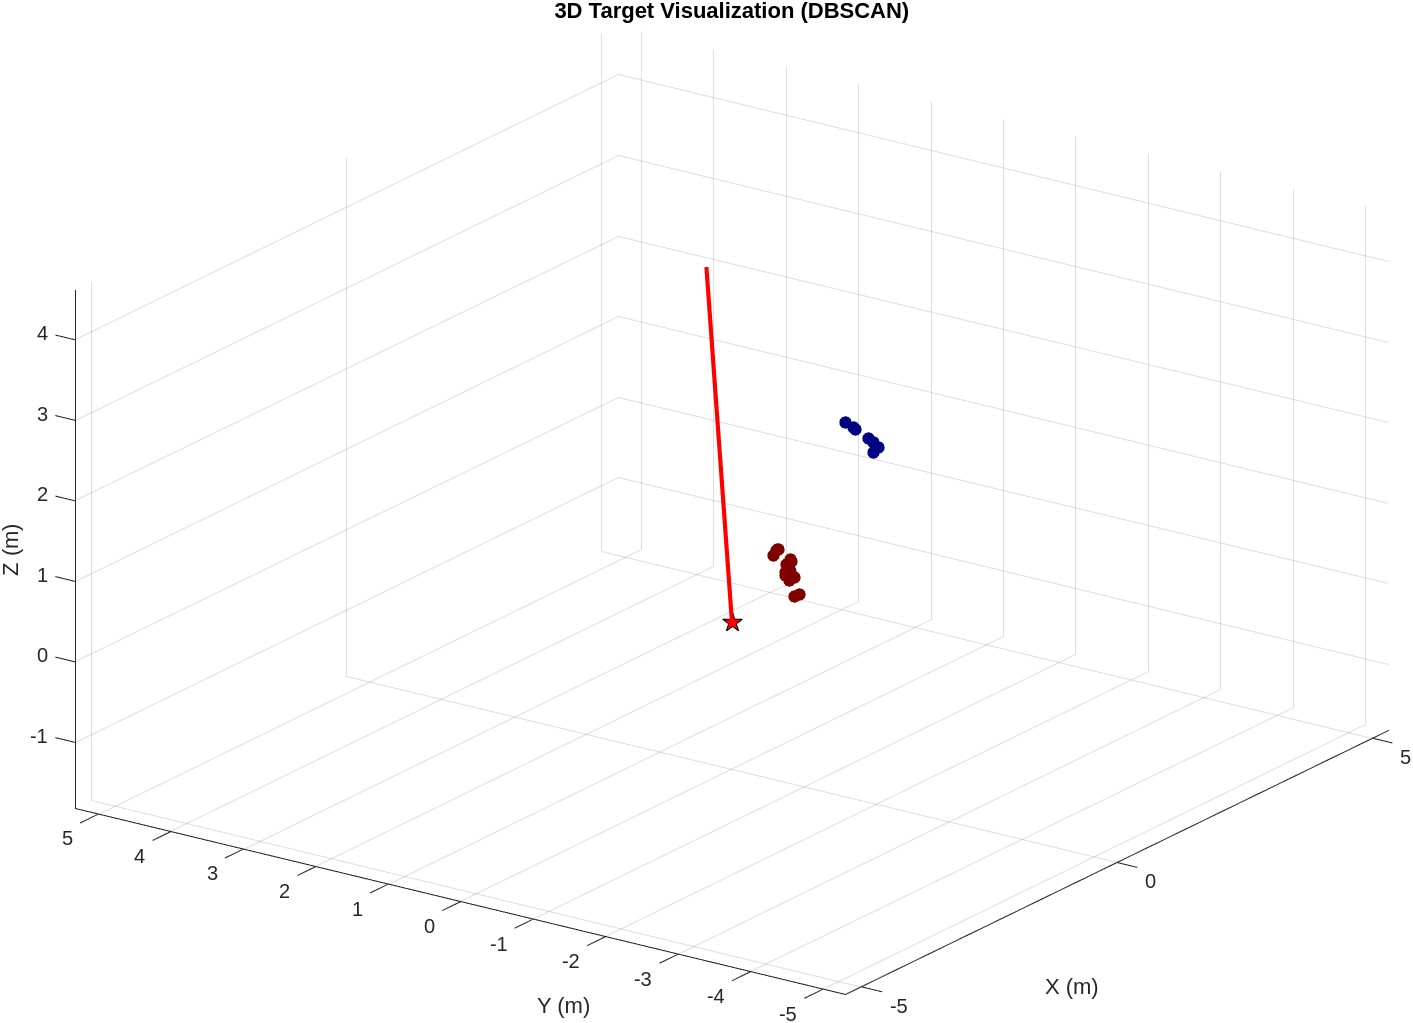
\includegraphics[width=0.9\textwidth]{../img/vis_3d.jpg}
	\caption[3D Space visualization method]{3D Space visualization method}
	\label{fig:vis3d}
\end{figure}

This visualization style is used to display CFAR data in 3D Cartesian space (Figure~\ref{fig:vis3d}).
The visualization method is rather simple, with just positions being recalculated from the range, azimuth, and pitch angles to x, y, and z coordinates using trigonometric functions.
If decay is enabled, then a small threshold is used to remove points whose values have sufficiently degraded.
To aid with orientation within the plot, the current heading of the platform is displayed as a red line.

If the environment is too cluttered and CFAR generates too many points, the user can enable basic clustering with MATLAB's built-in DBSCAN function \cite{matlab_dbscan}.
The general idea of DBSCAN is that, for a given point in the dataset, distances to other points are calculated and compared with a user-defined threshold $\varepsilon$.
If a sufficient number $N$ of points is found within the threshold, the point is marked as part of a cluster \cite{Kellner2012}.
In MATLAB's implementation, the distance threshold and minimum number of points are both configurable variables, with the other input being just the list of points \cite{matlab_dbscan}.
As the original data are in a polar coordinate system, a problem arises with calculating distances given that, in such a system, the distance between two points of given fixed yaw and pitch varies widely with range.
Not to mention, with increasing distance, the density of data points decreases.

These problems can be overcome using many different methods, such as using adaptive thresholds in relation to radius \cite{Kellner2012} or relying on more clever axis systems than just polar or Cartesian \cite{Sun2024}.
However, as in this thesis DBSCAN is more of an illustration of possible postprocessing, no such complex methods were implemented.
Both $\varepsilon$ and $N$ parameters are left to the user to configure with \texttt{DBSCAN epsilon} and \texttt{DBSCAN min count}.
As for the distance metric, points are first converted to Cartesian coordinates, then distance is calculated using the standard Euclidean formula.
This distance is then divided by the average radii of the points.
It needs to be said that, while dividing by the mean of distances is sometimes used when working with spherical data \cite{Fisher1993}, the author is not aware of any literature that would suggest its use in DBSCAN.
Especially at longer distances, this method will lead to significant errors.

\newpage
\pagestyle{plain}

% vim.ft=tex
\chapter*{Conclusion}
\addcontentsline{toc}{chapter}{Conclusion}

TODO


%%% Bibliography (literature used as a source)
%%%
%%% We employ biblatex to construct the bibliography. It processes
%%% citations in the text (e.g., the \cite{...} macro) and looks up
%%% relevant entries in the bibliography.bib file.
%%%
%%% See also biblatex settings in thesis.tex.

%%% Generate the bibliography. Beware that if you cited no works,
%%% the empty list will be omitted completely.

% We let bibliography items stick out of the right margin a little
\def\bibfont{\hfuzz=2pt}

\printbibliography[heading=bibintoc]

%%% If case you prefer to write the bibliography manually (without biblatex),
%%% you can use the following. Please follow the ISO 690 standard and
%%% citation conventions of your field of research.

% \begin{thebibliography}{99}
%
% \bibitem{lamport94}
%   {\sc Lamport,} Leslie.
%   \emph{\LaTeX: A Document Preparation System}.
%   2nd edition.
%   Massachusetts: Addison Wesley, 1994.
%   ISBN 0-201-52983-1.
%
% \end{thebibliography}


\listoffigures

\listoftables

\chapter*{Appendix}

\section*{Appendix A -- G-code glossary}

\setlist[itemize]{nosep, topsep=3pt, partopsep=3pt, leftmargin=*}
\setlist[description]{nosep, topsep=1pt, partopsep=1pt, leftmargin=*}

Following sections act as a glossary of all G-code commands used in the platform control. More in-depth descriptions of the commands can be found in the source code documentation.

\subsection*{Constants}

\begin{itemize}
  \item Parameters defined in Kconfig (require firmware recompilation):
  \item \texttt{STEPPER\_Y\_STEP\_COUNT}, \texttt{STEPPER\_P\_STEP\_COUNT}: Steps per rotation (modifiable via \texttt{M92}, non-persistent)
  \item \texttt{STEPPER\_[Y/P]\_PIN\_DIR}, \texttt{STEPPER\_[Y/P]\_PIN\_STEP}: GPIO pins for direction/step signals
  \item \texttt{STEPPER\_[Y/P]\_PIN\_ENDSTOP}: Endstop detection pins
  \item \texttt{STEPPER\_MAX\_SPEED}: Maximum RPM (hardware limit)
  \item \texttt{STEPPER\_DEFAULT\_SPEED}: Default motion RPM
  \item \texttt{STEPPER\_MIN\_SPINDLE\_TIME}: Minimum step interval of rotation in spindle mode
  \item \texttt{STEPPER\_HAL\_TIMER\_PERIOD/RESOLUTION}: PWM timer period/resolution, affects achievable RPM range
\end{itemize}

\subsection*{Features}

\begin{itemize}
  \item \textbf{Units}: Switch between degrees and steps using \texttt{G20}/\texttt{G21} respectively
  \item \textbf{Positioning Modes}:
    \begin{itemize}
      \item Absolute (\texttt{G90}): Automatically normalizes angles to [0, 360°] or [0, STEP\_COUNT]
      \item Relative (\texttt{G91}): Limited to $\pm$32767 steps per command, or respective angle counterpart
      \item in absolute positioning devices moves in the shortest path to the target
    \end{itemize}
  \item \textbf{Spindle}: Continuous rotation mode
  \item \textbf{Limits}: Limits on rotation can be imposed on both axes
    \begin{itemize}
      \item Limits are applied only to one rotation—it is not possible to restrict to, e.g., two full rotations in one direction and one in the other
      \item \texttt{low < high}: Valid range [low, high]
      \item \texttt{low > high}: Valid range [low, 360°] $\cup$ [0, high]
      \item Out-of-range targets snap to nearest valid position
    \end{itemize}
  \item \textbf{Programming}: G-code program can be uploaded to the device and executed
  \item \textbf{Synchronization}: If a command is issued to both axes, they will wait for each other; otherwise, the other axis will be free to execute the next command
\end{itemize}
\newpage

\subsection*{Motion Control Commands}

Axes are denoted as \texttt{Y} for yaw and \texttt{P} for pitch. The \texttt{S} parameter is used for speed for both axes, while \texttt{SY} and \texttt{SP} are used for the speed of yaw and pitch respectively. In the case of spindle, \texttt{Y} or \texttt{P} are not followed by step count/angle but instead by rotation direction.

\begin{description}
  \item[\texttt{M80}] Enable high-voltage power (enables drivers)
  \item[\texttt{M81}] Disable high-voltage power (disables drivers)
  \item[\texttt{M82}] Emergency stop (clears command queues)
  \item[\texttt{G20}] Set units to degrees
  \item[\texttt{G21}] Set units to steps
  \item[\texttt{G90 [Y/P]}] Set absolute positioning Mode
    \begin{itemize}
      \item Absolute positioning is not available in spindle mode; if you issue an M03 command to a stepper in absolute positioning mode, it will be automatically switched to relative positioning and throw an error
      \item If no argument is provided, both axes are switched to relative positioning
    \end{itemize}
  \item[\texttt{G91 [Y/P]}] Set relative positioning Mode
  \item[\texttt{G28 [Y/P]}] Auto-home specified axis(es)
  \item[\texttt{G92 [Y/P]}] Set current position as zero
  \item[\texttt{G0 Y<val> P<val> [SY/SP<rpm>]}] Stepper-mode movement
  \item[\texttt{M03 Y/P<+/-> [SY/SP<rpm>]}] Start spindle mode (continuous rotation)
  \item[\texttt{M05 [Y/P]}] Stop spindle mode
  \item[\texttt{M201 LY/HY/LP/HP<angle>}] Set angular limits (degrees/steps)
  \item[\texttt{M202 [Y/P]}] Disable limits
\end{description}

\subsection*{Special Commands}

These commands bypass certain sections and safety checks of the firmware. Use with caution.

\begin{description}
  \item[\texttt{G3 Y/P<steps> [SY/SP<rpm>]}] Bypass scheduler and adds movement directly to the queue
		\begin{itemize}
			\item Limits are not and cannot be checked
			\item Absolute positioning is not available
			\item All values are interpreted as steps regardless of current unit setting
			\item \textit{Warning}: Use \texttt{M82} before \texttt{G3} to maintain position integrity
		\end{itemize}
  \item[\texttt{W3 T<ms>}] Application-layer delay
		\begin{itemize}
			\item Useful to wait for end of homing process
		\end{itemize}
\end{description}

\subsection*{Programming Commands}
\begin{description}
  \item[\texttt{P90 <id>}] Start programming mode (overwrites existing program if any)
  \item[\texttt{P91}] Transition from header to main program body
  \item[\texttt{P92}] Finalize program (discarded if loops unclosed)
  \item[\texttt{P21 I<iterations>}] For-loop declaration
  \item[\texttt{P22}] End loop block
  \item[\texttt{P29}] Infinite loop marker (header only) - main body will be executed infinitely
  \item[\texttt{W0 Y/P<sec>}] Wait in seconds
  \item[\texttt{W1 Y/P<ms>}] Wait in milliseconds
\end{description}


\subsection*{Uplink Protocol}

\begin{itemize}
  \item \texttt{!P <timestamp>, <yaw>, <pitch>}: Position update (20ms interval)
  \item \texttt{!R OK}: Command acknowledgment
  \item \texttt{!R ERR <code>}: Command error
\end{itemize}

\begin{tabular}{ll}
  \hline
  \texttt{Code} & Description                          \\
  \hline
  1             & Malformed command syntax             \\
  2             & Invalid arguments                    \\
  3             & Queue lock failure                   \\
  4             & Unsupported command                  \\
  5             & System busy (homing/program running) \\
  6             & Runtime exception                    \\
  7             & Unclosed loop in program             \\
  8             & Invalid context                      \\
  \hline
\end{tabular}


\subsection*{Example Program}
\begin{tabular}{lll}
  \hline
  \texttt{Command}       & Mode   & Purpose                   \\
  \hline
  \texttt{P90 prog}      & Header & Initialize program ID=1   \\
  \texttt{G91}           & Header & Set relative positioning  \\
  \texttt{P29}           & Header & Enable infinite looping   \\
  \texttt{M03 SY6 Y+}    & Body   & Start Yaw spindle (6 RPM) \\
  \texttt{G0 SP30 P100}  & Body   & Pitch movement            \\
  \texttt{G0 SP30 P-100} & Body   & Return pitch              \\
  \texttt{P92}           & Body   & Finalize program          \\
  \hline
\end{tabular}


\clearpage
\openright
\end{document}
